\pdfminorversion=4 % for compliance with 1a-b

\begin{filecontents*}[overwrite]{\jobname.xmpdata}
  \Title{Dissertation}
  \Author{Andrii Nikolaiev}
  \Language{uk-UA}
  \Subject{Development of Data Synthesis and Mathematical Combinatorial Problem Generation Methods Using Large Language Models}
  \Keywords{Artificial intelligence\sep automated theorem proving\sep natural language processing\sep large language models\sep machine learning\sep mathematical problems}
\end{filecontents*}

\documentclass[type=phd]{mon2017dev}

% % ——— disable all images (graphicx draft mode) ———
% \PassOptionsToPackage{draft}{graphicx}

\usepackage[a-1b]{pdfx}

% % Removing transparency
% \pdfpageattr{/Group<</S/None/CS/DeviceRGB>>}
% \usepackage{graphicx}
% \setkeys{Gin}{interpolate=false}

\usepackage{setup}
% \usepackage{refcheck} % checking the presence of all references used

\begin{document}
% Назва дисертації

\title{Розроблення методів синтезу даних та генерації математичних комбінаторних задач за допомогою великих мовних моделей}
	
	% Прізвище, ім'я, по батькові здобувача
 
\author{Ніколаєв Андрій Дмитрович}
	
	% Факсимільний підпис автора у файлі sorokina-sig.pdf, .eps, .jpeg тощо
	% (зсув по x, зсув по y)
	% [параметри команди \includegraphics]
	% \facsimilesig{author}(-60,-12)[width=70pt]{sorokina-sig}
	
	% Прізвище, ім'я, по батькові наукового керівника/консультанта
 
\supervisor{Анісімов Анатолій Васильович}{доктор фізико-математичних наук, професор}
	
%	\speciality(uk){122}  % шифр спеціальності
%	\speciality(en){122}
	
	% Індекс за УДК
 
\udc{004.8}
	
	% Установа, де виконана робота, і місто
 
\institution{Київський національний університет імені Тараса Шевченка\\Міністерство освіти і науки України\\Київський національний університет імені Тараса Шевченка\\Міністерство освіти і науки України}{Київ}
	
	% Команду \council переписано в стилі команди \institution:
	% ключ institution задає «стандартну» назву установи, у спеціалізованій вченій раді якої проводиться захист дисертації
	% (з вказуванням назви органу, до сфери управління якого належить заклад, установа),
	% а ключ altname — «альтернативну» (тобто скорочену, для анотації).
	% Якщо факультативний аргумент відсутній, то клас вважає,
	% що захист проводиться в тій самій установі, де здійснювалася підготовка здобувача,
	% а отже, немає потреби писати назву цієї установи двічі на титульному і в анотації.
	% Але за потреби можна вручну повторити тут назву установи, і буде повтор на титульному і в анотації.
 
%	\council(uk){ДФ~41.052.021}
%	\council(en){ДФ~41.052.021}
	
	% Рік, коли написана дисертація
\date{2025}
	% LC_CTYPE=cp1251 luit grep -ro -P cite\{.*?\}
	
	% Тут буде титульний аркуш
\maketitle
\newpage
%
\addtocontents{toc}{\setcounter{tocdepth}{-1}}
\chapter*{Анотація}
\addtocontents{toc}{\setcounter{tocdepth}{2}}

\emph{Ніколаєв~А.Д.} Розроблення методів синтезу даних та генерації математичних комбінаторних задач за допомогою великих мовних моделей.~\textbf{\textemdash}~Кваліфікаційна наукова праця на правах рукопису.

Дисертація на здобуття наукового ступеня доктора філософії за спеціальністю 122 «Комп'ютерні науки».~\textbf{\textemdash}~КНУ ім. Тараса Шевченка, Київ, 2025.

У даній дисертаційній роботі досліджуються можливості використання великих мовних моделей для синтезу даних та генерації математичних комбінаторних задач. Основна мета дослідження полягає у виявленні можливостей великих мовних моделей до математичного міркування та розробки ефективних методів до генерації синтетичних даних, що зберігають математичну сутність задач.

У роботі запропоновано нові методи генерації варіацій математичних комбінаторних задач шляхом модифікації їхніх конфігурацій, лінгвістичних та стилістичних особливостей. Проведено серію експериментальних досліджень на створених даних, та оцінено ефекти впливу синтезованих даних на ефективність роботи великих мовних моделей та відповідності до людських результатів експертів з олімпіадно-математичним досвідом.

\textbf{Основні результати та наукова новизна роботи}:
\begin{itemize}
    \item Розроблено метод синтезу даних на основні систематичної маніпуляції текстів математичних комбінаторних задач задля порівняння ефективності великих мовних моделей та експертів з олімпіадним досвідом у міркуванні.
    \item Розроблено метод генерації математичних комбінаторних задач шляхом класифікації, відбору та створення нових синтетичних варіацій задач зі збереженою математичною сутністю за допомогою великих мовних моделей та запровадження метрики варіаційної узгодженості текстів задач.
\end{itemize}

Результати дослідження демонструють значний потенціал великих мовних моделей у завданні генерації комбінаторних задач зі збереженням математичної сутності, що відкриває нові можливості для розробки методів автоматичної формалізації математичних текстів. Основним викликом для використання мовних моделей залишається забезпечення точності генерації розв'язань, адже як було продемонстровано у експериментальній частині, мовні моделі мають високий рівень чутливості до змін тексту за допомогою додаткових маніпуляцій з текстами задач, таких як додавання зайвої числової інформації, зміни конфігурації параметрів задачі та лінгвістично-стилістичної модифікації умов текстів задач. Задля подальшого поліпшення систем автоматичного пошуку доведень запропоновано метод інтеграції мовних моделей із формальними методами для символічних обчислень.

За результатами експериментальної частини були досягнуті наступні результати:
\begin{enumerate}
    \item Проведено огляд систем штучного інтелекту та сучасних методів обробки природної мови, проаналізовано та розглянуто кілька видів архітектур моделей, методів з використанням технік для побудови міркувань, задіяння додаткових інструментів для символьної обробки даних, а також існуючих наборів даних та метрик оцінювання.
    \item Розроблено набір даних \emph{Combi-Puzzles}, який включає набір з 125 комбінаторних задач з систематичною модифікацією умов за допомогою керування наступними параметрами та особливостями задач: конфігурація задачі, внесення додаткової зайвої інформації, зміна лінгвістично-стилістичної формату тексту.
    \item Проведено експериментальне порівняння ефективності моделей до розв'язання математичних комбінаторних задач на синтезованих даних та оцінено близько 36 тис. відповідей моделей на основі набору критеріїв для перевірки коректності логічних міркувань моделей при генерації тверджень під час розв'язання математичних комбінаторних задач та оцінено чутливість мовних моделей до модифікацій текстів задач.
    \item Проведено серію експериментальних досліджень з участю 35 учасників з олімпіадним досвідом, отримано та проаналізовано більше 800 розв'язків задач, які були використані при порівняльному аналізі результатів роботи моделей та експертів.
    \item За допомогою розроблених методів відбору, генерації та оцінки якості синтетичних даних для комбінаторних задач за допомогою великих мовних моделей було згенеровано більше 20 тис. екземплярів математичних комбінаторних задач.
\end{enumerate}

\emph{Ключові слова}: штучний інтелект, автоматизовані системи доведень, обробка природної мови, великі мовні моделі, машинне навчання, математичні задачі.

\newpage

%
\addtocontents{toc}{\setcounter{tocdepth}{-1}}
\chapter*{Abstract}
\addtocontents{toc}{\setcounter{tocdepth}{2}}

\emph{Nikolaiev~A.D.} Development of Data Synthesis and Mathematical Combinatorial Problem Generation Methods Using Large Language Models. ~\textbf{\textemdash}~Qualification scientific work on the rights of the manuscript.

The PhD thesis on competition for a scientific degree of the doctor of philosophy in the speciality 122 \say{Computer~Science}.~\textbf{\textemdash}~Taras Shevchenko National University of Kyiv, Kyiv, 2025.

This dissertation investigates the use of large language models for data synthesis and the generation of mathematical combinatorial problems. The primary goal of the research is to investigate the mathematical reasoning capabilities of these models and to develop effective methods for generating synthetic data that preserves the mathematical essence of the problems.

The study introduces novel techniques for creating variations of mathematical combinatorial problems by modifying their configurations as well as their linguistic and stylistic characteristics. A series of experiments was conducted on the generated data to evaluate the impact of synthesised problems on the performance of large language models and to compare their outcomes with those achieved by experts with Olympiad-level mathematical experience.

\textbf{Main results and scientific contributions:}
\begin{itemize}
    \item A data synthesis method based on systematic manipulation of the texts of mathematical combinatorial problems was developed to compare the reasoning performance of large language models with that of experts possessing Olympiad-level experience.
    \item A novel method for generating variations of mathematical combinatorial problems was proposed. This approach involves the classification, selection, and creation of new synthetic variations that preserve the mathematical essence of the problems, utilising large language models and introducing a variation consistency metric.
\end{itemize}

The findings demonstrate the significant potential of large language models in generating combinatorial problems that maintain their mathematical integrity, thereby opening up new avenues for the automatic formalisation of mathematical texts. A key challenge remains to ensure the accuracy of generated solutions; as shown in the experimental section, language models exhibit high sensitivity to modifications in the problem texts, including the addition of irrelevant numerical information, changes in problem configuration, and linguistic-stylistic alterations. To further improve automated proof-search systems, the dissertation proposes integrating language models with formal symbolic computation techniques.

Based on the experimental studies, the following achievements were realised:
\begin{enumerate}
    \item A comprehensive review of artificial intelligence systems and modern natural language processing methods was conducted. This included an analysis of various model architectures, reasoning techniques, the use of auxiliary tools for symbolic data processing, as well as existing datasets and evaluation metrics.
    \item The \emph{Combi-Puzzles} dataset was developed, comprising 125 combinatorial problems with systematic modifications of problem conditions by controlling parameters such as problem configuration, the injection of redundant information, and changes in the linguistic-stylistic format of the problem statements.
    \item An experimental comparison of the model performance in solving mathematical combinatorial problems on synthesised data was performed. Approximately 36,000 model responses were evaluated using a set of criteria designed to verify the correctness of logical reasoning during the generation of problem statements, along with an assessment of the models' sensitivity to text modifications.
    \item A series of experiments involving 35 participants with Olympiad-level experience was carried out, and an analysis of over 800 problem solutions that were conducted for the comparative evaluation of the performance of models and experts.
    \item Utilising the developed methods for the selection, generation, and quality evaluation of synthetic data for combinatorial problems, more than 20,000 instances of mathematical combinatorial problems were generated.
\end{enumerate}

\emph{Keywords}: artificial intelligence, automated theorem proving, natural language processing, large language models, machine learning, mathematical problems.

\addtocontents{toc}{\setcounter{tocdepth}{-1}}
\chapter*{Список публікацій здобувача}
\addtocontents{toc}{\setcounter{tocdepth}{2}}

\medskip
\textit{\textbf{Наукові праці, в яких опубліковані основні наукові результати дисертації:}}
\medskip

\begin{enumerate}
    \item Ніколаєв, Андрій Д. та Анісімов, Анатолій В. \textit{Нейромережеві методи відбору та генерації синтетичних варіацій комбінаторних задач}. Кібернетика та системний аналіз. 2025, том 61, випуск 3, с.22-32. DOI: \url{https://doi.org/10.34229/KCA2522-9664.25.3.3}.
    \item Ніколаєв, Андрій. \textit{Нейромережеві методи формалізації математичних текстів}. Herald of Khmelnytskyi National University. Technical sciences, 345.6(2), 2024, с. 50—55. DOI: \url{https://doi.org/10.31891/2307-5732-2024-345-6-6}.
    \item Nikolaiev, Andrii D. та Derevianchenko, Oleksandr V. \textit{Comparison of Problem-solving Performance Across Mathematical Domains With Large Language Models}. Shtuchnyy intelekt, 2024, с. 96—104. \url{https://doi.org/10.15407/jai2024.04.096}.
    \item Власенко, О.В., Картавих, В.Ю., Ніколаєв, А.Д., Горбенко, В.І. \textit{Методика визначення опорної матриці моніторингу домена управління інформаційної мережі спеціального призначення}. Системи і технології зв’язку, інформатизації та кібербезпеки. Збірник наукових праць ВІТІ, випуск 4, 2019, с. 46—57.
\end{enumerate}

\medskip
\textit{\textbf{Наукові праці, які засвідчують апробацію матеріалів дисертації:}}
\medskip

\begin{enumerate}
    \item \textit{Introducing constraints in combinatorial problems: A case study with LLaMA 3.1}. -- 11th International Scientific Conference "Information Technology and Implementation (IT\&I-2024 Satellite)". Taras Shevchenko National University of Kyiv, 2024.
    \item \textit{AI in education: Application of LLMs for learning mathematics.} -- Ukrainian Cambridge: New Research by Displaced Scholars from Ukraine. University of Cambridge, 2023.
    \item Nikolaiev, Andrii D. and Anisimov, Anatoliy V. \textit{Mathematical word problem solution evaluation via data preprocessing approach}. 8th International Scientific Conference "Information Technology and Implementation (IT\&I-2021)", Vol. 3132, 2022, p. 94—103. \url{https://ceur-ws.org/Vol-3132/Paper_9.pdf} %\url{https://www.scopus.com/inward/record.uri?eid=2-s2.0-85129578190&partnerID=40&md5=63f41d66fe66b0b9088484ef474dcd4e}
    \item \textit{Implementation of Artificial Intelligence Module for Educational Purposes}. -- 7th International Scientific Conference "Information Technology and Interactions (IT\&I-2020 Satellite)". Taras Shevchenko National University of Kyiv, 2020.
\end{enumerate}

\medskip
\textit{\textbf{Наукові праці, які додатково відображають наукові результати дисертації:}}
\medskip
\begin{enumerate}
    \item Nikolaiev, Andrii, Stathopoulos, Yiannos та Teufel, Simone. \textit{Can language models rival mathematics students? Evaluating mathematical reasoning through textual manipulation and human experiments}. arXiv preprint, 2024. \url{https://arxiv.org/abs/2412.11908}.
\end{enumerate}

\tableofcontents
% Перелік умовних позначень
\chapter*{Перелік умовних позначень}

\begin{longtable}{p{3cm}p{11cm}}
    ШІ & Штучний інтелект (Artificial Intelligence) \\
    ВММ & Великі мовні моделі (Large Language Models) \\
    NLP & Обробка природної мови (Natural Language Processing) \\
    MWP & Математичні текстові задачі (Mathematical Word Problems) \\
    SAD & Системи автоматизації доведень (System for Automated Deduction) \\
    RNN & Рекурентні нейронні мережі (Recurrent Neural Network) \\
    FNN & Нейронні мережі прямого поширення (Feedforward Neural Network) \\
    CoT & Ланцюжок міркувань (Chain-of-Thought) \\
    GPT & Генеративний попередньо навчений трансформер (Generative Pre-trained Transformer) \\
    RLHF & Навчання з підкріпленням на основі людського зворотного зв'язку (Reinforecement Learning from Human Feedback) \\
    RAG & Генерація з доповненням через пошук (Retrieval-Augmented Generation) \\
    ToRA & Інтегроване розуміння з інструментами (Tool-integrated Reasoning Agents) \\
    CPU & Центральний процесор (Central Processing Unit) \\
    GPU & Графічний процесор (Graphical Processing Unit) \\
    API & Прикладний програмний інтерфейс (Application Programming Interface)
\end{longtable}

\newpage

\chapter*{Вступ}

\paragraph{Обґрунтування вибору теми дослідження.}

Математичне міркування є фундаментальним аспектом освіти та наукових досліджень. Здатність розв'язувати складні математичні задачі є критичною не лише в математиці, але й у різних галузях, таких як фізика, інженерія, комп'ютерні науки, економіка, біологія тощо. Традиційно, математичне міркування вимагало людської експертизи, значного обсягу досвіду та вміння працювати з формальними типами даних.

З розвитком штучного інтелекту (ШІ) та методів обробки природної мови (Natural Language Processing, NLP) з’явилися великі мовні моделі (ВММ), які демонструють вражаючі результати в аналізі, розумінні та генерації тексту. Сучасні моделі, такі як новітні версії GPT і LLaMA, досягли значного прогресу у вирішенні різноманітних завдань у роботі з текстом, зокрема й з математичними задачами.

Застосування ВММ для синтезу та генерації математичних текстів відкриває нові можливості. З одного боку, ВММ можуть обробляти великі обсяги даних та виявляти закономірності у великих масивах даних та приходити до висновків, які можуть використовувати задля автоматичної формалізації текстів та генерації розв'язань задач. Проте з іншого боку, математичне міркування вимагає точних математичних обчислень, дедукції, а також можливості працювати з абстрактними концепціями. Незважаючи на те, що великі мовні моделі демонструють вражаючі результати у розв'язанні математичних задач, більшість цих результатів базується на запропонованих наборах задач та не може бути ефективно доводити адекватність моделей. Для підтвердження даного факту необхідно створити унікальний набір математичних задач, який не було використано для попереднього навчання даних моделей.

Задля ефективної демонстрації обмеження моделей та оцінки їхніх можливостей, у даній роботі було проведено дослідження з математичними комбінаторними задачами, які незважаючи на звичайний текстовий вигляд мають прихований математичний підтекст -- питання або задачу, що потребує здатності моделей до ефективного міркування та пошуку відповідних підходів для розв'язання.

Виконання поставленої задачі передбачає огляд сучасного стану проблеми, підготовки даних, проведення експериментів з залученням людини та сучасних версій ВММ з проведенням аналітичної частини дослідження.

\paragraph{Мета та завдання дослідження}
Метою дисертаційної роботи є дослідити застосування великих мовних моделей для розробки методів синтезу математичних даних та генерації математичних комбінаторних задач.
Для досягнення поставленої мети було поставлено наступні завдання:

\begin{enumerate}
    \item Проаналізувати сучасний стан моделей штучного інтелекту та методів обробки природної мови для роботи з математичними задачами, що включає огляд архітектур, формальних методів, методів машинного навчання, існуючих наборів даних та метрик для оцінювання ефективності роботи моделей.
    \item Розробити власний набір математичних комбінаторних задач з новими варіаціями через систематичні модифікації текстів оригінальних задач.
    \item Провести експериментальне дослідження для визначення впливу характеристик математичних задач на ефективність роботи великих мовних моделей із залученням експертної оцінки.
    \item Розробити та впровадити метод генерації синтетичних текстів задач за допомогою великих мовних моделей.
    \item Здійснити порівняльний аналіз ефективності моделей у генерації математичних текстів.
\end{enumerate}

\textbf{Об'єктом дослідження} є моделі штучного інтелекту та методи обробки природної мови для роботи з математичними текстовими задачами.
\medskip

\textbf{Предметом дослідження} є методи синтезу даних та генерації математичних комбінаторних задач за допомогою великих мовних моделей.
\medskip

\textbf{Методи дослідження} включать: методи обробки природної мови з використанням багатошарової нейромережевої архітектури на основі людського зворотного зв’язку, навчання з підкріпленням, моделей-експертів та інших підходів; техніки побудови запитів; методи статичного аналізу та обробки даних.

Обчислювальні ресурси та інструменти: Експерименти проводилися з використанням графічних процесорів Nvidia A100, Nvidia Quadro RTX 8000, а також серверних потужностей компанії OpenAI з доступом до моделей через API; для експериментів використовувалися версії великих мовних моделей GPT-4, LLaMA, Qwen, Mistral у кількох версіях та розмірах; для розробки програмного забезпечення було використано мову програмування Python 3.11 із відповідними бібліотеками для роботи з даними та мовними моделями.

\medskip

\paragraph{Наукова новизна отриманих результатів}

У дисертаційній роботі проведено комплексне дослідження можливостей великих мовних моделей для генерації математичних комбінаторних задач, зокрема порівняння з ефективності різноманітних мовних моделей, людей-експертів, проведення аналізу числових та стилістичних особливостей текстів задач. Запропоновано нові методи генерації синтетичних даних та метрики оцінки якості згенерованих даних.

Протягом вирішення поставлених задач дослідження, вперше отримані наступні результати:
\begin{itemize}
    \item Розроблено метод синтезу математичних комбінаторних задач зі збереженою сутністю шляхом відбору та систематичної маніпуляції текстів задач за рахунок контролю параметрів та стилістичних особливостей задач, на основі якого створено новий набір задач.
    \item Вперше проведено експеримент з участю людей-експертів з олімпіадним математичним досвідом задля проведення оцінювання здатності моделей до розв'язання варіацій комбінаторних задач та чутливості до модифікацій текстів.
    \item Запроваджено нову метрику варіаційної узгодженості текстів задач, що дозволяє оцінювати якість синтетичних даних та їхню відповідність оригінальним текстам.
\end{itemize}

\paragraph{Важливість та практичне значення отриманих результатів}

Отримані результати підтверджують високий потенціал великих мовних моделей у генерації математичних текстів та удосконаленні систем автоматизованого пошуку доведень. Розроблені методи синтезу даних та генерації математичних комбінаторних задач не лише підвищують ефективність автоматизованих підходів до створення математичних задач, а й відкривають нові можливості для інтеграції нейромережевих технологій із формальними методами обчислень.

Проведена робота є важливим внеском у сучасні дослідження штучного інтелекту, які спрямовані на автоматизацію математичної освіти та розвиток ефективних систем доведень, і створюють основу для подальших наукових розробок у сфері обробки природної мови та аналізу математичних даних.

Окрім використання отриманих результатів для подальшого поліпшення математичних можливостей ВММ, вони закладають основу до розробки адаптивних навчальних систем та інтеграції моделей штучного інтелекту у освіту та наукові дослідження.

% Перевірити та оновити перед публікацією.
\paragraph{Структура та обсяг дисертаційної роботи}

Дисертація складається зі вступу, чотирьох розділів, кожен з яких завершується підсумками, висновків, списку використаних джерел та додатків. Загальний обсяг роботи складається з 142 сторінок, з яких основний зміст викладено на 112 сторінках. Робота містить 44 рисунка, 25 таблиць та список використаних джерел посилань із 91 найменувань.

\newpage

% Розділи
\graphicspath{{./data/}}
\chapter{Огляд методів та архітектур моделей штучного інтелекту для обробки математичних задач}

Одним з напрямків обробки природної мови є робота з математичними текстами – задачами, які можуть бути розв'язані за допомогою різноманітних методів, включаючи класифікаційні алгоритми, глибоке навчання та системи пошуку доведень. Класифікація та вивчення різних типів таких задач, а також аналіз методів до їх розв'язання, є необхідними для ефективного пошуку відповідних систем та вдосконалення механізмів розпізнавання умов задач.

У загальному вигляді математичні текстові задачі (Mathematical Text Problems, MWP) -- це задачі, які представлені природною мовою та вимагають математичного міркування для розв'язання. Зазвичай дані задачі подаються у вигляді тексту або разом з додаткового зображення. Вони є важливим інструментом для оцінки розуміння математичних можливостей систем, а також мають практичне значення у реальних ситуаціях.

Особливість розробки ефективних систем пошуку доведень полягає у тому, щоб обробити текст задач та коректно ідентифікувати важливі елементи інформації задля того, щоб продемонструвати логічну послідовність та точність у висновках.

\section{Різновиди математичних задач}

Перед тим як перейти до огляду методів роботи з математичними текстами задач опишемо деякі типи задач та їхні особливості.

Математичні текстові задачі (MWP) є поширеним типом задач, які використовуються при розробці систем автоматичного пошуку розв'язань. Класифікувати задачі можна за форматом (задачі з варіантами відповіді, розгорнуті розв'язання, короткий розв'язок тощо) або за математичними розділами (наприклад, геометрія, алгебра, комбінаторика тощо):

\begin{itemize}
    \item Задачі типу Multiple Choice (MCQ-type Questions)
    \item Алгебраїчні задачі (Algebra Problems)
    \item Геометричні задачі (Geometric Problems)
    \item Задачі на теорію чисел (Number Theory problems)
    \item Комбінаторні задачі (Mathematical Combinatorial Problems)
\end{itemize}

Окрім інших типів задач, які не наведені вище, слід зазначити, що деякі математичні задачі можуть мати властивості відразу кількох тем, наприклад, так звані комбі-геометричні задачі -- задачі, які задані у просторі певної розмірності, але передбачають певний комбінаторний підхід до їх розв'язання. Наведемо більш детальний опис відповідних типів задач.

\paragraph{Задачі з вибором кількох варіантів відповідей}
Розв'язання задач цього типу починається з аналізу текстової умови, що дозволяє ідентифікувати ключові математичні об'єкти та логічні зв'язки, присутні в задачі. Система виконує генерацію або вибір з попередньо визначеного набору можливих відповідей, після чого проводиться ретельна оцінка кожного варіанту. Використання класифікаторів або експертних правил дозволяє обрати правильну відповідь, спираючись на порівняння виділених характеристик умови з можливими відповідями. Таким чином, основна задача полягає у побудові моделі, здатної на основі вхідного тексту оцінити релевантність кожного варіанту. Здебільшого даний тип задач не є складним, адже надає обмежену кількість варіантів (зазвичай від 4 до 10) до вибору відповідей системою.  Задачі даного типу досліджуються як окремий тип за рахунок формату поданих умов, але можуть включати різні тематики (геометрія, алгебра і тд.).

\paragraph{Алгебраїчні задачі}
Алгебраїчні задачі є важливою категорією, оскільки вони вимагають трансформації текстового опису у відповідні математичні вирази та рівняння, що відображають логічну структуру задачі. До цієї категорії належать, зокрема, арифметичні словесні задачі та задачі зі системами рівнянь. Дані підтипи є найбільш активно досліджуваними завдяки їх відносній структурованості та ясності математичного моделювання, що дозволяє застосувати як символьні, так і чисельні методи розв'язання.

У розв'язанні \textbf{арифметичних словесних задач} важливо перетворити текстовий опис у математичну модель. Спочатку проводиться автоматичне відокремлення числових параметрів, операцій та невідомих, що містяться в умові. Далі формується відповідне алгебраїчне рівняння або система рівнянь, що відображає логічну структуру задачі. Для отримання точного розв'язання застосовуються як символьні, так і чисельні методи обчислення, що дозволяє перевірити коректність отриманого результату. Такий підхід об'єднує в собі можливості NLP для аналізу тексту та традиційні методи розв'язання рівнянь.

Даний тип задач характеризуються тим, що за допомогою даних текстових умов необхідно скласти відповідне рівняння та отримати відповідь на задачу. Такі задачі задаються послідовністю слів $\langle w_0, w_1, \dots, w_k \rangle$, де деякі слова є кількостями $q_0, q_1, \dots, q_n$, згаданими в тексті, а також невідомою змінною $x$. Основною метою є подання текстової задачі у вигляді відповідного рівняння $E$, яке є лінійним у даному випадку. Серед основних арифметичних операцій використовуються лише $+$, $-$, $\times$, $\div$. Арифметичні задачі були одними з перших, які досліджувалися у даній галузі за рахунок простоти у перевірці коректності складених рівнянь.

\begin{figure}[h]
    \centering
    \small
    \captionof{table}{Приклад арифметичної словесної задачі. Кольором виділені елементи задачі, які мають інформаційну цінність до запитання або є зайвими.}
    \label{tab:mwp_example}
    \begin{tabular}{|p{0.38\linewidth}|p{0.31\linewidth}|p{0.13\linewidth}|}
        \hline
        \textbf{Умова задачі} & \textbf{Рівняння до умови задачі} & \textbf{Числова відповідь} \\
        \hline
        Міша знайшов \hlgreen{35 мушель} та \hlred{7 морських зірок} на пляжі. Він віддав \hlgreen{22 мушлі} Каті. Скільки мушлей тепер має Міша? & \[ x = 35 - 22 \] & \[ 13 \] \\
        \hline
    \end{tabular}
\end{figure}

Задачі, що включають \textbf{системи рівнянь}, вимагають виділення декількох пов'язаних умов, кожна з яких може бути формалізована як окреме рівняння. Після цього будується система рівнянь, яка описує взаємозв'язок між невідомими величинами. Розв'язання таких систем може здійснюватися як символьними методами (наприклад, методом Гауса), так і чисельними алгоритмами, що дозволяє адаптувати модель до конкретних вимог задачі. Важливим аспектом є точність математичного моделювання та правильне перетворення семантичної інформації тексту у математичну форму. Дані задачі активно використовуються у задачах оптимізації.

\paragraph{Геометричні задачі}
Геометричні задачі орієнтовані на просторове мислення та вимагають особливого підходу до інтерпретації описаних у задачі геометричних об'єктів. Спершу здійснюється розпізнавання опису геометричних фігур, відрізків, кутів або інших просторових характеристик. На основі цього формується математична модель, що може містити геометричні формули для обчислення довжини, площі або об'єму. У деяких випадках задача може вимагати інтеграції з візуальними методами обробки даних, якщо поряд із текстом подається схематичне зображення. Таким чином, застосовуються як класичні геометричні алгоритми, так і сучасні методи глибокого навчання для аналізу просторових описів.

\paragraph{Задачі з теорії чисел}
Задачі з теорії чисел охоплюють широкий спектр задач, що досліджують властивості цілих чисел, такі як простота, дільники, залишки та інші властивості чисел. Розв'язання таких задач зазвичай вимагає застосування спеціалізованих теорем та алгоритмів, спрямованих на аналіз властивостей чисел. Система, яка обробляє подібні задачі, повинна мати можливість розпізнавати ключові поняття, трансформувати текстовий опис у формалізовану модель та застосовувати як символьні методи доказу, так і чисельні алгоритми для перевірки результатів. Активно досліджуваними аспектами є алгоритми щодо перевірки простоти чисел, обчислення найбільшого спільного дільника, а також застосування евристичних методів.

\paragraph{Комбінаторні задачі}
До цієї категорії відносяться задачі, які не підпадають безпосередньо під попередні типи розв'язання. Вони можуть вимагати комплексного підходу, який об'єднує декілька математичних та алгоритмічних методів для побудови адекватної моделі задачі. При розв'язанні таких задач особливо значущим є здатність моделей до відокремлення семантичної складової задачі задля пошуку необхідних теорем чи термінів, які нададуть можливість перевести задачу у формально-математичному вигляді. У деяких випадках поєднується символьний аналіз із моделями глибокого навчання для точного визначення послідовності логічних кроків. Інтеграція результатів різних методів забезпечує підвищення цієї загальної точності та дозволяє розв'язати складні задачі, що містять неоднозначності або вимагають комплексного аналізу.

Комбінаторні задачі добре підходять для оцінки математичних можливостей моделей штучного інтелекту та систем автоматичного пошуку доведень, оскільки правильні відповіді зазвичай виражені як комбінаторні формули або у звичайному числовому вигляді, що робить процес перевірки відповіді ефективним та відтворюваним. Формулювання відповідей на комбінаторні задачі може включати біноми, факторіали та інші комбінаторні символьні представлення, які також приймаються в експерименті. Приклад комбінаторної задачі з відповіддю в обох формах наведено в Таблиці~\ref{table:puzzle_example}.

\begin{figure} \centering \small
    \captionof{table}{Приклад комбінаторної задачі з відповіддю.}
    \label{table:puzzle_example}
    \begin{tabular}{|p{0.38\linewidth}|p{0.31\linewidth}|p{0.13\linewidth}|}
        \hline
        \textbf{Умова задачі} & \textbf{Комбінаторна відповідь} & \textbf{Числова відповідь} \\
        \hline
        Ліа має 2 яблука, 3 банани і 2 апельсини. Наступного тижня вона хоче з'їсти по одному фрукту кожного дня. Скільки існує способів це зробити? & \[ P(2,3,2) = \frac{7!}{2!3!2!} \] & \[ 210 \] \\
        \hline
    \end{tabular}

\end{figure}

Крім того, при наданні відповіді у вигляді комбінаторної формули зазвичай можливо витягти кроки міркування, які призвели до фінальної відповіді. Також існує можливість знайти комбінаторні задачі з широким діапазоном складності, які можуть бути додатково налаштовані за допомогою різних текстових маніпуляцій. Ці характеристики роблять комбінаторні задачі ефективним та практичним способом оцінки математичних міркувань.

Детальні описи наборів даних математичних задач та їхні застосування наведені у Розділі~\fullref{sec:datasets}.

\section{Традиційні методи розв'язання математичних задач}

Системи автоматизації доведень (САД) призначені для перевірки та генерації математичних доведень шляхом формального логічного виведення. 

\subsection{Системи автоматизації доведень}

Оцінювання можливостей штучного інтелекту виконувати завдання на математичне міркування є важливою і складною галуззю досліджень, особливо при розв'язуванні математичних текстових задач. Ця область є широкою і охоплює різні формати задач, включаючи арифметичні задачі, відповіді на запитання з множинним вибором, відповіді на математичні запитання і генерацію розв'язків математичних текстових задач. Останнє включає в себе проблеми обробки природної мови, зокрема розуміння тексту і генерацію логічно послідовних висновків, та підкреслює потребу в ефективних методах оцінювання ефективності методів до вирішення даної задачі. Перші методи були запропоновані за допомогою формальних систем, таких як автоматизовані системи доведення теорем.

Понад 50 років тому, у 1970-х роках, академік В.М. Глушков опублікував статтю, в якій обговорював різні виклики штучного інтелекту та представив дослідницьку програму під назвою ``Алгоритм Очевидності'' \cite{glushkov1970some}. У цій програмі було викладено його бачення комп'ютеризованої діяльності людини з пошуку доведень теорем. Глушков запропонував зосередитися на створенні системи для автоматизації пошуку доведень теорем. Це передбачало розробку формальних мов для написання математичних текстів у природному для людини форматі, створення процедур пошуку доведень на основі розширюваного концепту очевидності комп'ютера, використання наявних або новонабутих знань, і надання інтерфейсів для користувачів, щоб покращити роботу з системою \cite{Glushkov1970, Glushkov1972}. З моменту публікації було здійснено дві основні спроби реалізувати дану програму. Перший привів до появи системи автоматизації доведень у 1980 році \cite{glushovsad1980}, а другий привів до її англомовної модифікації, System for Automated Deduction (SAD), у 2002 році \cite{10.1007/978-3-540-73595-3_29}. Також з'явилися  інші автоматизовані системи доведення теорем, які використовували формальні системи, такі як Isabelle \cite{paulson1986natural} (1989) та Lean \cite{demoura2015lean} (2001).

\subsection{Формалізація текстів}

Формалізація текстів -- це процес перетворення математичних висловлювань, заданих природною мовою, у формальний синтаксис, зрозумілий для САД. Це складний процес, який вимагає врахування семантичних та синтаксичних особливостей математичної мови.

Системи, що згадуються вище, мають високу точність і забезпечують логічно послідовну структуру для математичних доведень. Зазвичай вони вимагають повністю формалізованих даних, які можуть бути оброблені САД, але не є зручними для розуміння людиною. У статті \cite{10.1007/978-3-540-85110-3_47} автори запропонували формалізувати дані мовою ForTheL, яка підтримує структуру математичної аргументації у природному мовному вигляді, але при цьому придатна для автоматизованої обробки відповідними САД. Однак будь-яка підготовка даних у формалізований спосіб, як зазначають автори набору олімпіадних даних з математики FIMO \cite{liu2023fimochallengeformaldataset}, вимагає значних зусиль від експертів і великих витрат.

\subsection{Обмеження формальних методів}

Недоліком традиційних САД є необхідність ручної формалізації текстів, що є трудомістким процесом і вимагає високої кваліфікації від користувача. Як зазначають \cite{liu2023fimochallengeformaldataset}, основними складнощами для роботи з текстом є:

\begin{itemize}
    \item {Висока вартість формалізації.} Сфера формальних математичних даних характеризується бідністю, оскільки створення формальних математичних даних вимагає значних зусиль від експертів, а отже, має значну вартість. Наприклад, навіть один з найбільших репозиторіїв формальної математики, mathlib, спільна ініціатива, спрямована на створення єдиної математичної бібліотеки в Lean, має лише 45 МБ у розмірі. На противагу цьому, процес підготовки GPT-3 використовує широкий набір даних CommonCrawl \cite{brown2020languagemodelsfewshotlearners}, який, навіть після фільтрації, охоплює колосальні 570 ГБ, перевищуючи розмір mathlib більше ніж у 10,000 разів.
    
    \item {Низький рівень складності існуючих наборів даних.} Існуючі формальні набори даних часто тяжіють до нижчих рівнів складності, що може перешкоджати моделям у набутті необхідних навичок. Наприклад, відомий набір даних miniF2F пропонує набір задач зі складністю рівня міжнародної математичної олімпіади (IMO). Задачі рівня IMO за визначенням мають підвищену складність, і слід зазначити, що лише кілька прикладів були успішно розв'язані автоматизованими системами пошуку доведень \cite{polu2020generativelanguagemodelingautomated, zheng2022minif2fcrosssystembenchmarkformal, han2022proofartifactcotrainingtheorem, wang-etal-2023-dt}.
    
    \item {Неповнота даних.} Більшість формальних математичних наборів даних пропонують лише формальні твердження, нехтуючи відповідними твердженнями або доказами в природних мовах. Ця відсутність не лише компрометує інтерпретацію тверджень, але й заважає системам пошуку доведень з використанням нейронних мереж використовувати доведення на природних мовах, цінне джерело, яке часто доступне для олімпіадних математичних завдань середньої школи.
\end{itemize}


%%%%%%%%%%%%%%%%%%%%%%%%%%%%%%%%%%%%%%%%%%%%%%%%%%%%%%%%%%%%%%%%%%%%%%%%%%%%%%

\section{Підходи до розв'язання математичних задач на основі методів обробки природної мови}

Методи обробки природної мови (Natural Language Processing, NLP) зосереджені на розробці технологій та систем, здатних аналізувати, інтерпретувати та генерувати текст у природній формі. Ця галузь охоплює широкий спектр завдань, зокрема пошукові системи, машинний переклад і текстову аналітику, що значно розширюють можливості мовних моделей.

Розв'язання математичних задач з природної мови є активною областю досліджень у сфері NLP та систем автоматичного пошуку доведень. Існує кілька методів до розв'язання таких задач, кожен з яких має свої переваги та обмеження. Подальше вдосконалення цих методів дозволить створювати більш точні та ефективні системи для автоматизованого розв'язання математичних задач.

Ранні методи до розв'язання математичних задач з природної мови можна класифікувати на три основні категорії: статистичний, допомогою дерев та на основі глибокого навчання. Більш ранні методи, які були засновані на наборах правил, будуть опущені для зосередження на сучасніших методах. Деякі методи також використовують комбінацію вищезгаданих категорій.

\subsection{Ранні методи з використанням обробки природної мови}

\paragraph{Статистичний методи}
Статистичний підхід намагається ідентифікувати сутності питання, їхні значення та необхідні оператори для обчислення правильної відповіді. Для ідентифікації використовуються загальні методи машинного навчання.

Наприклад, у роботі \cite{hosseini-etal-2014-learning} запропоновано метод розв’язання арифметичних текстових задач, що містять операції додавання та віднімання. Запропонована система ARIS аналізує кожне речення задачі, визначаючи відповідні змінні та їхні значення. Потім ці дані перетворюються на рівняння, яке формалізує задачу та дозволяє отримати розв’язок шляхом послідовного оновлення станів до завершення процесу.

Інший підхід використовується \cite{mitra-baral-2016-learning}, які застосували кероване навчання для визначення формули, яка повинна бути застосована для генерації відповідного рівняння та релевантних змінних.

\paragraph{Метод за допомогою дерев}
Метод за допомогою дерев фокусується на представленні задачі у ієрархічній формі. Ієрархію задає унікальне дерево, відоме як бінарне дерево виразів. Дерево виразів може бути оцінене шляхом застосування оператора на кореневому вузлі до значень, отриманих шляхом рекурсивного оцінювання лівого та правого піддерев.

Наприклад, \cite{koncel-kedziorski-etal-2015-parsing} запропонували систему ALGES, яка генерує дерево над простором усіх можливих дерев виразів, яка враховує арифметичні задачі з однією формулою як відповіддю.

Інші автори представили метод дерева виразів (Expression Tree), який робить декомпозицію математичної задачі на декілька класифікаційних проблем, а потім складає відповідне дерево виразів \cite{roy2016solvinggeneralarithmeticword}.

\paragraph{Підхід на основі глибокого навчання}
У методі на основі глибокого навчання використовуються нейронні мережі для моделювання та розв'язання математичних задач. Ці методи включають як рекурентні нейронні мережі (Recurrent Neural Network, RNN), а також мережі з використанням механізму уваги, про який буде уточнено пізніше.

Наприклад, інші автори запропонували MathDQN, який є модифікованою формою загальної рамки глибокого підкріпленого навчання \cite{Wang_Zhang_Gao_Song_Guo_Shen_2018}. Вони визначили дії, стани та функцію винагороди, використовуючи нейронну мережу прямого поширення (Feedforward Neural Network, FNN).

Іншим прикладом, є модель Seq2Seq, яка включає кодувальник та декодувальник для генерації шаблонів лінійних рівнянь \cite{wang2018translatingmathwordproblem}.

\subsection{Методи представлення мови}

\begin{figure}[!h]
    \centering
    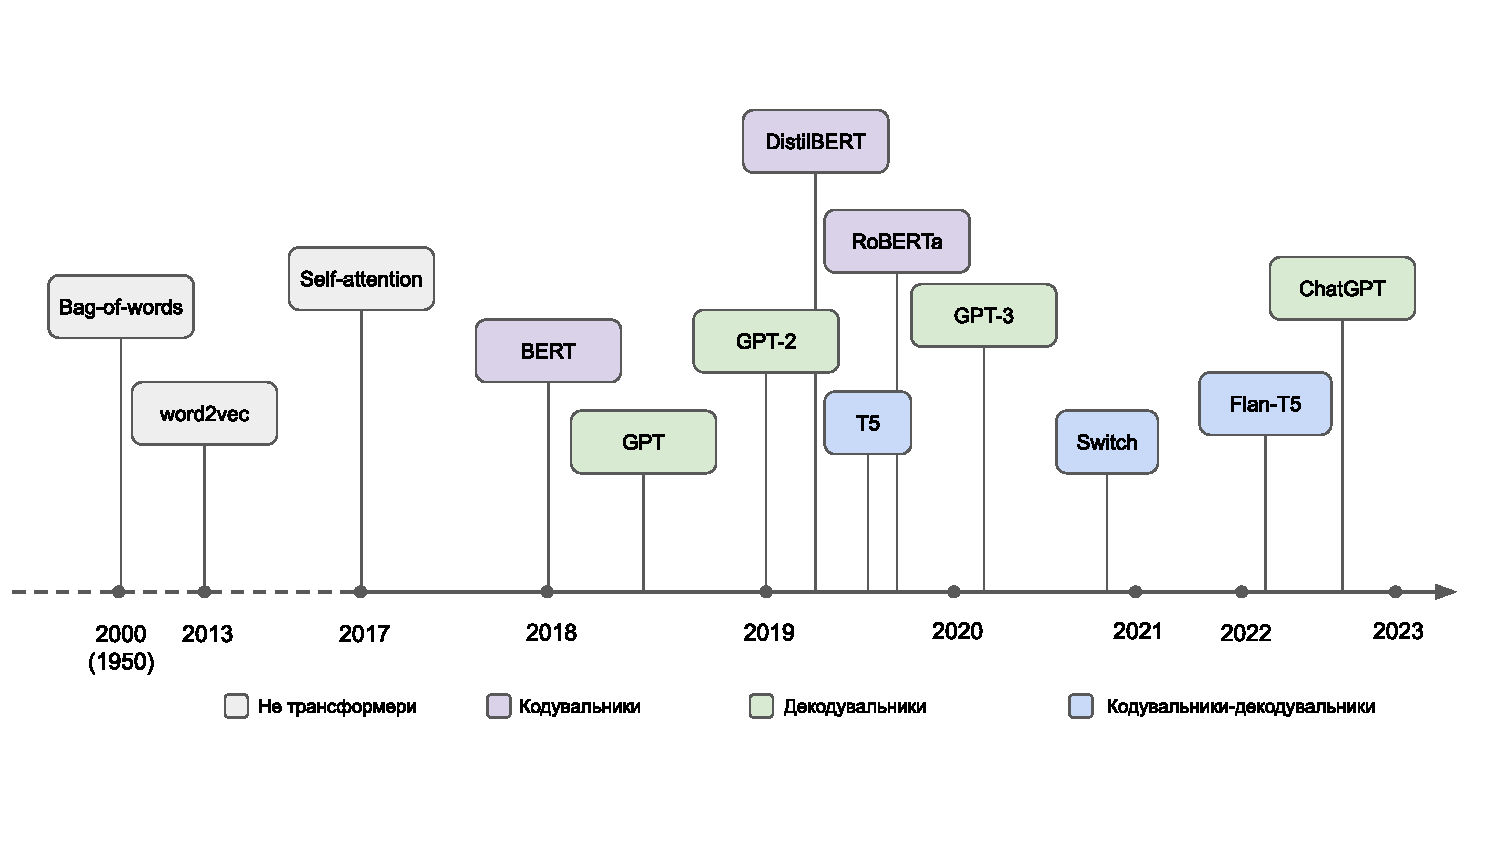
\includegraphics[width=1.0\textwidth]{lang_ai_history.pdf}
    \caption{Історія розвитку методів обробки природної мови за останні 25 років.}
    \label{fig:peek_language_ai}
\end{figure}

Еволюція методів обробки природної мови обумовлена низкою концептуальних і технологічних результатів, спрямованих на розробку систем представлення та генерації природної мови. На рис.~\ref{fig:peek_language_ai} можна бачити історію розвитку NLP у останні 25 років, ілюструючи основні моменти, які поєднують перші спрощені методи з сучасними трансформерними моделями.

Як показано на \ref{fig:lang-ai-tasks}, сучасні технології мовного ШІ застосовуються у широкому діапазоні завдань – від обробки текстового вводу для перекладу до генерації зв’язного тексту в діалогових системах. Оскільки звичайне текстове подання (послідовність чисел) є неструктурованим і втрачає свою смислову інформацію, науковці зосереджують увагу на розробці методів перетворення текстових даних у структуровані числові представлення, що забезпечують ефективну комп'ютерну обробку.

\begin{figure}[!h]
    \centering
    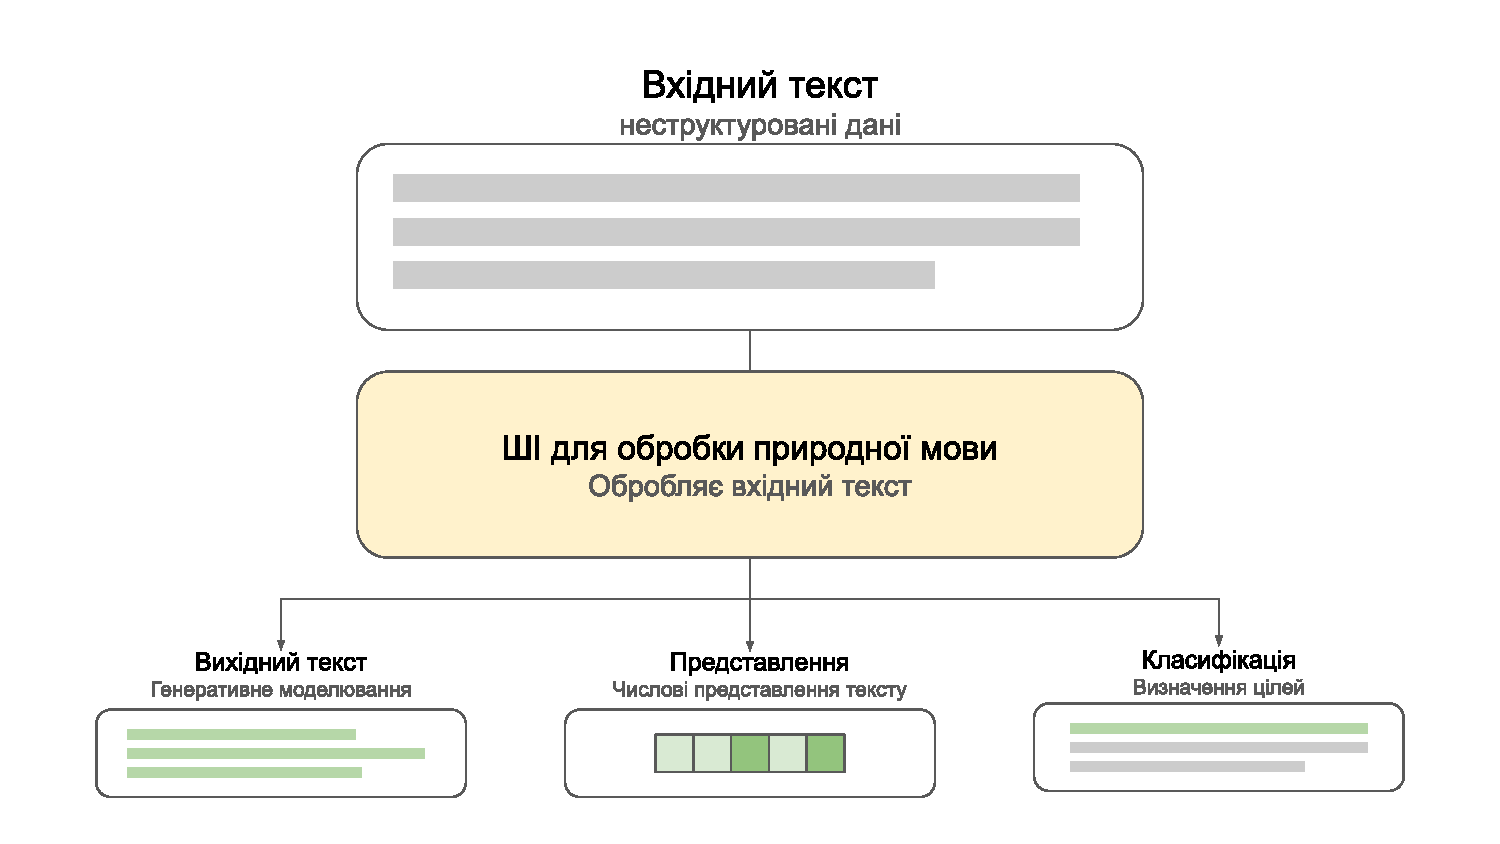
\includegraphics[width=0.8\textwidth]{lang_ai_tasks.pdf}
    \caption{Деякі завдання методів обробки природної мови.}
    \label{fig:lang-ai-tasks}
\end{figure}

\paragraph{Метод мішка слів.}

Перші дослідження в області методів обробки природної мови спиралися на методах представлення тексту без врахування його синтаксичної та семантичної структури або звичайне кодування слів. Метод ``мішка слів'' (bag-of-words), який уперше згадувався ще у 1950-х роках і набув популярності з 2000-х, полягає у перетворенні тексту у вигляді вектору, який утворюється шляхом підрахунку кількості появ кожного унікального слова.

\begin{figure}[!h]
    \centering
    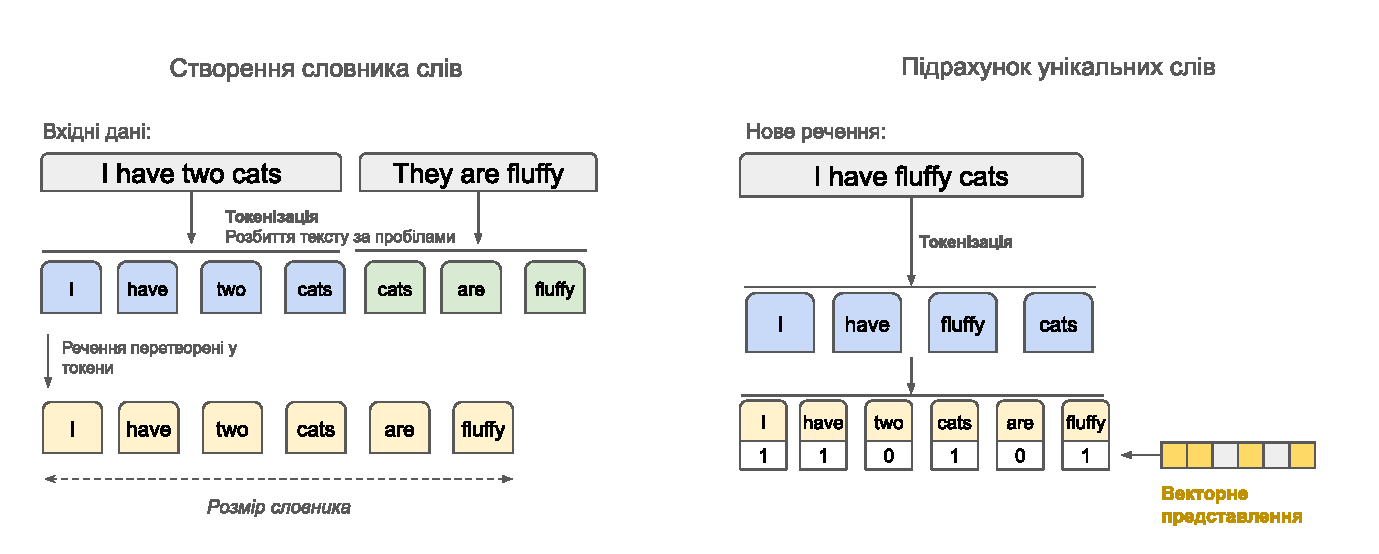
\includegraphics[width=1.0\textwidth]{bow.pdf}
    \caption{Метод ``мішок слів'': токенізація тексту шляхом розбиття за пробілами, формування словника слів та представлення нового вхідного речення у векторному вигляді.}
    \label{fig:bow}
\end{figure}

На рис.~\ref{fig:bow} можна бачити візуалізацію метода ``мішка слів''. На першому кроці відбувається етап токенізації, на якому формується словник з усіх унікальних слів зі вхідних даних. Після цього, коли на вхід отримується нове речення, підрахунок появи кожного слова дозволяє створити векторне представлення тексту за допомогою словника. Попри те, що даний підхід є спрощеним і не відображає семантичну особливості тексту, він заклав основу для подальшого розвитку методів представлення мови.

\paragraph{Векторні представлення слів}
З розвитком методів NLP, почали враховуватися більш динамічні властивості мови, такі як \emph{семантичні (semantic)} та \emph{контекстні (contextual)} особливості слів. Семантика визначає значення слів, фраз і речень незалежно від їхнього текстового оточення, фокусуючись на лексичних та синтаксичних правилах мови. Натомість контекст охоплює мовні та позамовні фактори, що впливають на інтерпретацію значення, зокрема попередні речення, дискурс або інші особливості вживання. Таким чином, семантика забезпечує базове розуміння змісту, тоді як контекст дозволяє враховувати нюанси використання слів та їхнього визначення.

Відповідно наступним кроком у розвитку обробки мовних даних стало використання векторного представлення слів -- \emph{ембединги (word embeggings)}. Метод word2vec, запропонований у 2013 році, полягає в присвоєнні кожному слову фіксованого за розміром вектору, який кодує його семантичні властивості. Це дозволяє за допомогою вимірювання відстаней у векторному просторі оцінювати семантичну подібність між словами.

Процес навчання векторних представлень слів відбувався за допомогою нейронних мереж, які представляють набір шарів та відповідних зв'язків між ними. На кожній ітерації тренування мережа отримує пару слів із текстового корпусу і намагається передбачити, чи є ці слова сусідніми у реченні. В процесі навчання відбувається оптимізація параметрів нейронної мережі (ваги зв'язків), завдяки чому слова з подібними семантичними значеннями отримують близькі ембединги як у прикладі на рис.~\ref{fig:nn_predictions}.

\begin{figure}[!h]
    \centering
    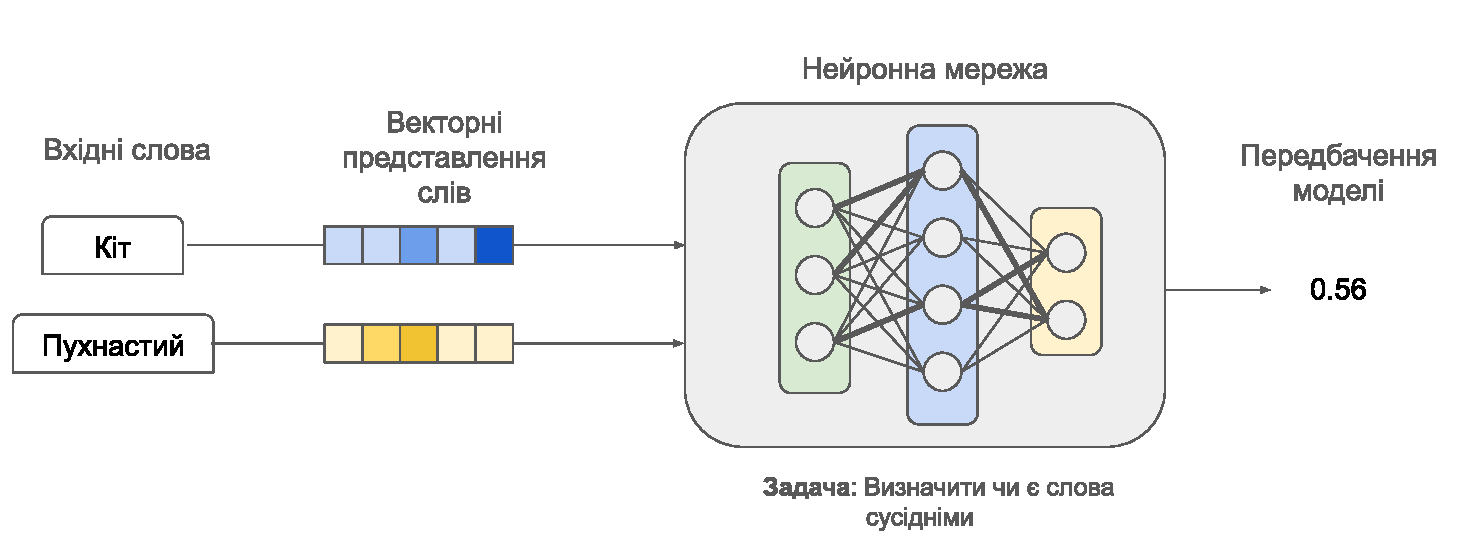
\includegraphics[width=1.0\textwidth]{nn_predictions.pdf}
    \caption{Навчання нейронної мережі шляхом передбачення сусідства слів.}
    \label{fig:nn_predictions}
\end{figure}

Отримані ембединги слів дозволяють описати семантичні властивості слів: наприклад, слово ``кіт'' може набувати високих значень за характеристиками ``тварина'' та ``пухнастість'', тоді як ``гвинтокрил'' матиме низькі значення за цими показниками. Як представлено на рис.~\ref{fig:embeddings} за рахунок векторного представлення відповідні слова можна візуалізувати слів у просторі з метою визначення семантичної близькості між словами.

\begin{figure}[!h]
    \centering
    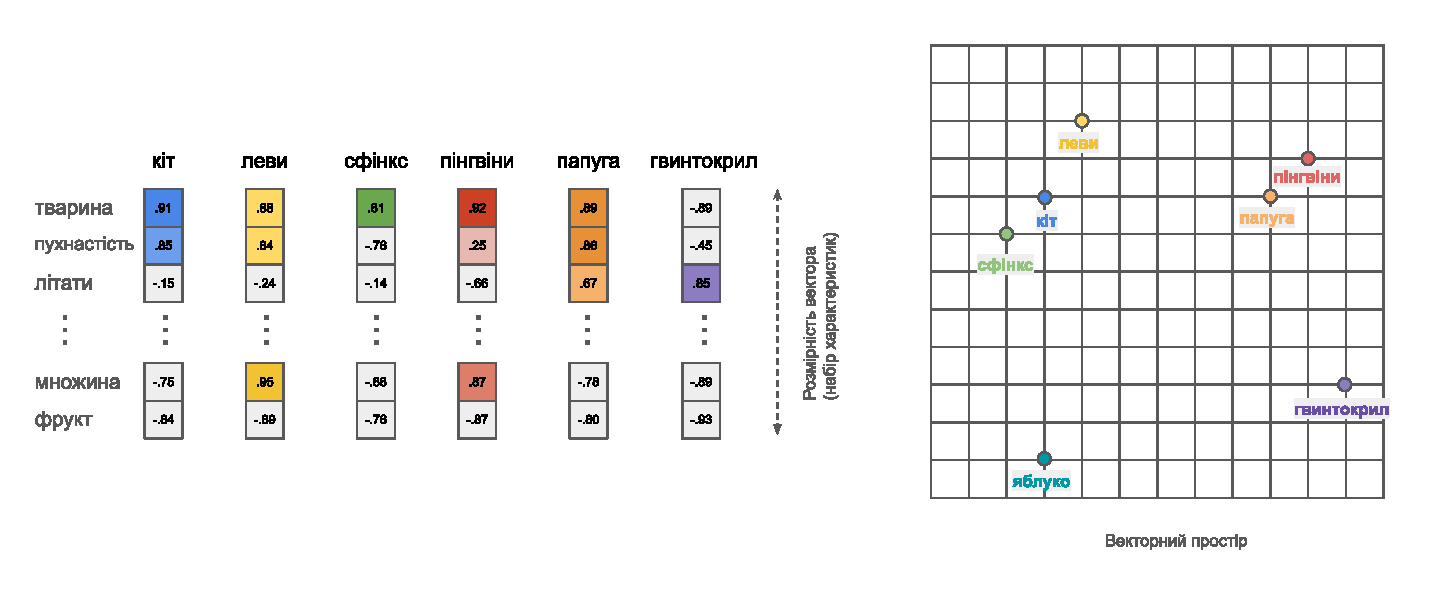
\includegraphics[width=1.0\textwidth]{embeddings.pdf}
    \caption{Ембединги слів, що задають властивості слів та їхня візуалізація у двовимірному просторі. Слова, що мають більше спільних характеристик, знаходяться ближче у просторі.}
    \label{fig:embeddings}
\end{figure}

Слід також зазначити, що існують різні типи векторних представлень даних, що відображають різноманітні рівні абстракції тексту -- від представлення окремих слів до представлення цілих речень або документів.

\paragraph{Кодування та декодування семантики тексту з використанням рекурентних нейронних мереж.}

Перші методи, такі як word2vec, створювали статичні представлення слів, де кожне слово має однаковий вектор значень незалежно від їхньої контекстної інформації (значення слів в залежності від вживання у відповідному реченні). Проте такий підхід не є оптимальним, адже багато слів можуть мати кілька семантичних значень. Наприклад, слово ``замок'' може означати як пристрій для обмеження доступу, так і укріплена будівля

Для врахування семантики слів спочатку застосовувалися рекурентні нейронні мережі (Recurrent Neural Network, RNN). За допомогою RNNs відбувався послідовний процес кодування та декодування заданого тексту. На рис.~\ref{fig:autoregressive_rnn} ілюструється процес генерації перекладу вихідного речення англійською мовою: ``I have two cats'' -- у перекладі українською: ``У мене є два кота''. Даний процес є авторегресійним (autoregressive), тобто кожен попередньо згенерований токен передається на вхід для генерації решти тексту.

\begin{figure}[!h]
    \centering
    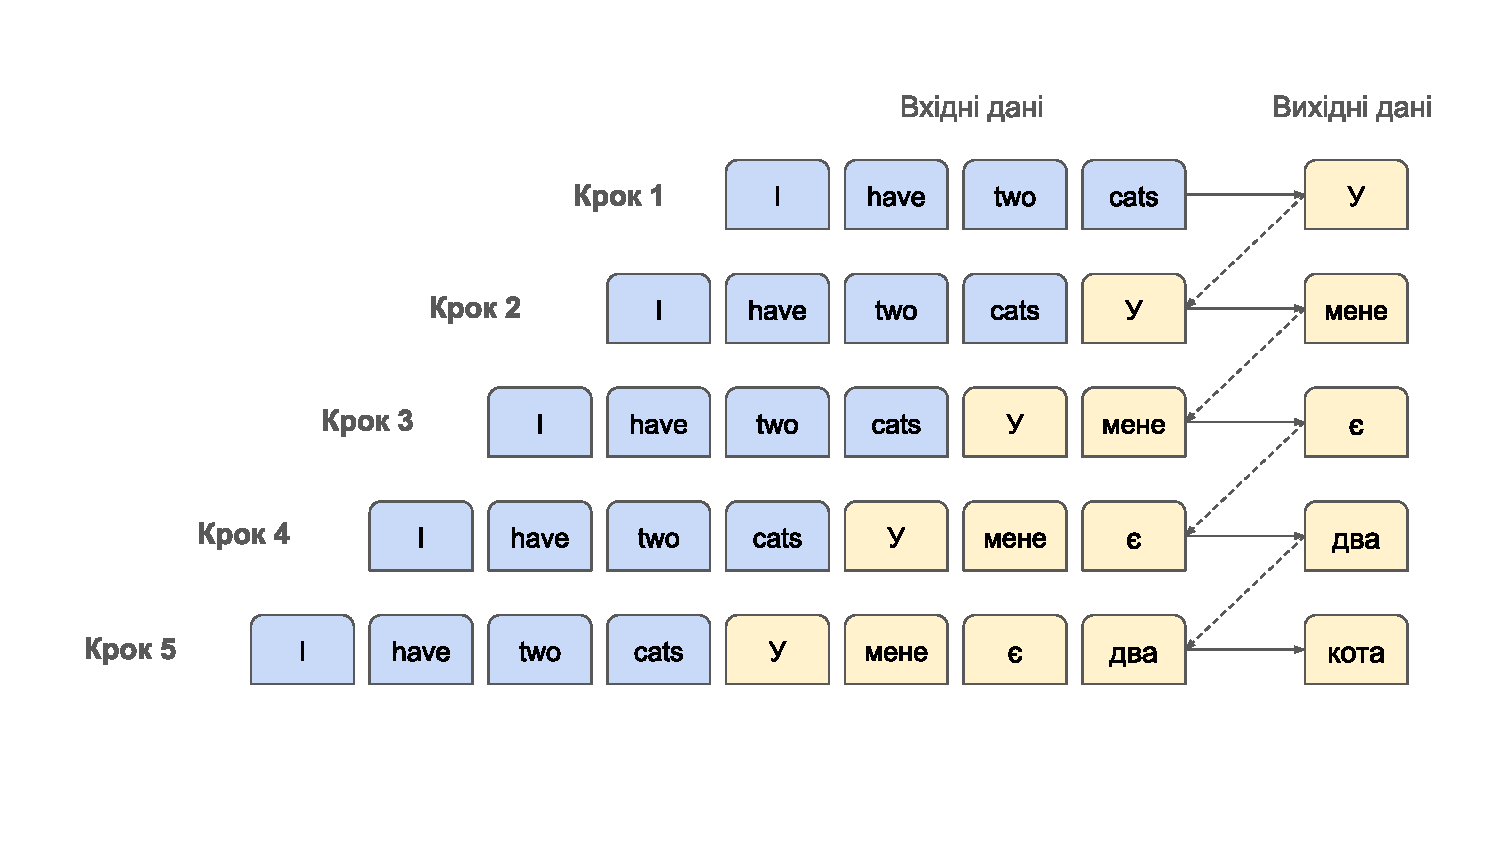
\includegraphics[width=0.9\textwidth]{autoregressive_rnn.pdf}
    \caption{Авторегресійний підхід під час генерації з використанням RNN: Кожен щойно згенерований токен використовується для генерації наступних токенів.}
    \label{fig:autoregressive_rnn}
\end{figure}

У даному методі з метою створення векторного представлення повного речення, на початому етапі були використані ембединги слів методом word2vec, приклад відповідної архітектури та процес обробки вхідного речення можна бачити на рис.~\ref{fig:context_embedding_word2vec}).

\begin{figure}[h]
    \centering
    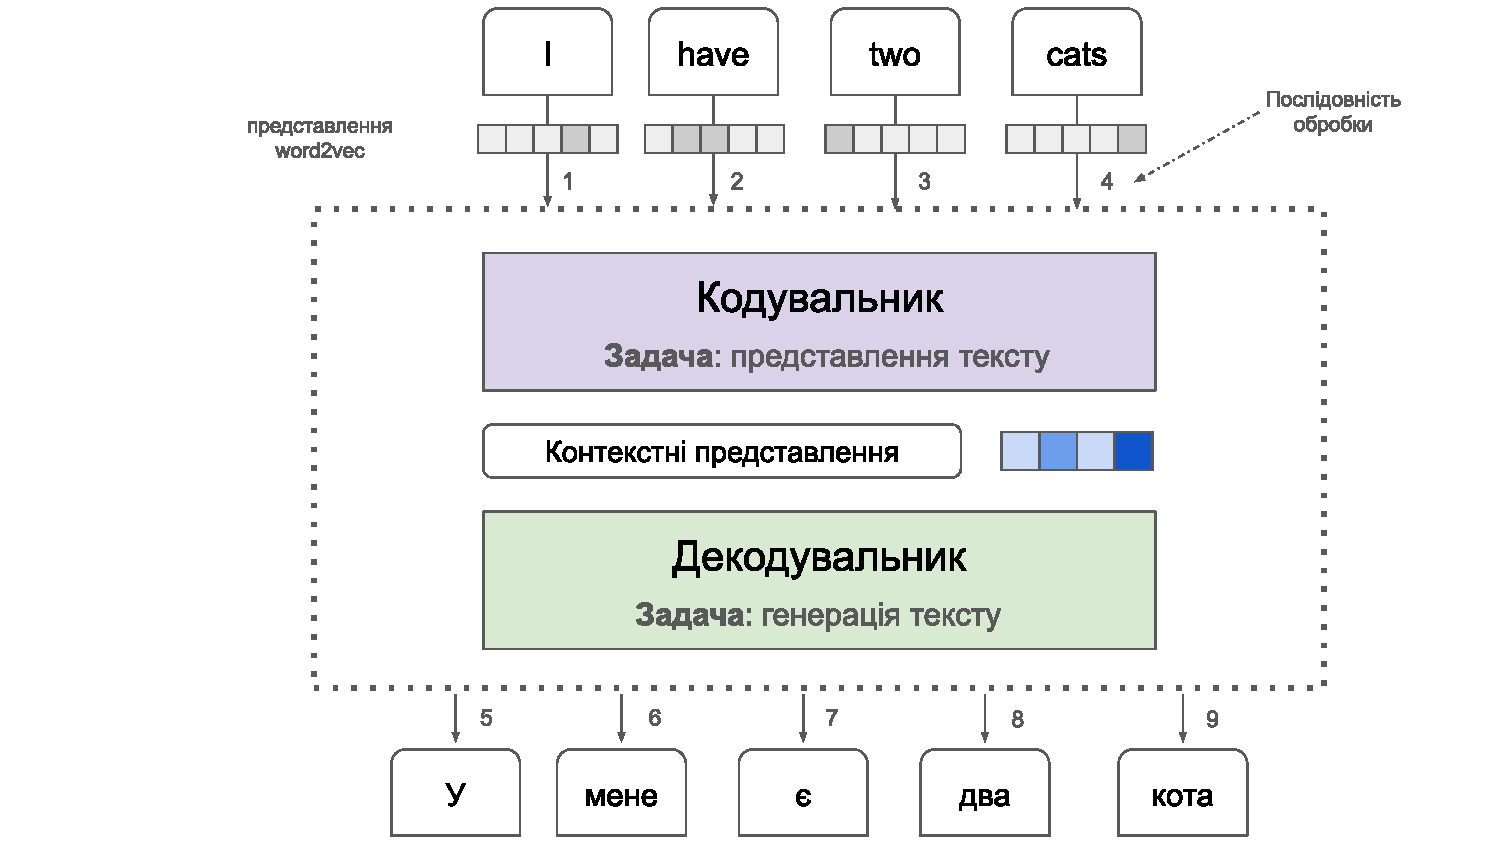
\includegraphics[width=0.9\textwidth]{context_embedding_word2vec.pdf}
    \caption{Формування загального представлення речення на основі векторних представлень слів методом word2vec.}
    \label{fig:context_embedding_word2vec}
\end{figure}

\paragraph{Механізм уваги}
Загальне представлення слів word2vec, як зображено на рис.~\ref{fig:context_embedding_word2vec}, ускладнює обробку речень. Дані ембединги не є чутливими до різноманітного вживання слів при побудові речень, тому відповідно не передають тонкощів задля розуміння текстів. У 2014 році було запропоновано рішення, яке називається \emph{механізм уваги (attention)}, що значно покращило якість векторного представлення текстів. Механізм уваги дозволив моделям зосередитись на частинах речення, які є релевантними до відповідних слів під час побудови перекладу, як зображено на рис.~\ref{fig:attention}. Механізм уваги вибірково визначає, які залежності між словами вхідного та вихідного речення є найбільш суттєвими. Наприклад, вихідне слово ``two'' українською значить ``два'', саме тому ступінь уваги між цими словами є високою. Аналогічно, наприклад, слова ``cats'' та ``мене'' мають нижчий рівень залежності, оскільки вони є менш пов’язаними між собою.

\begin{figure}[h]
    \centering
    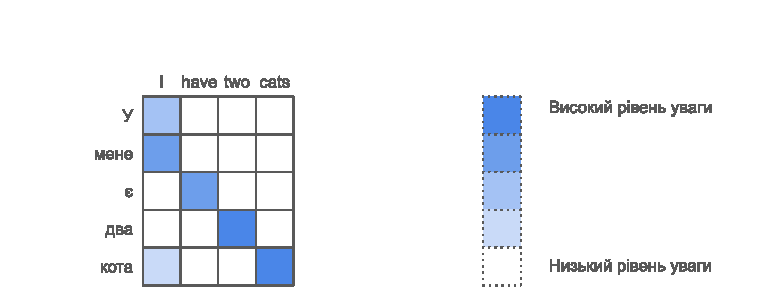
\includegraphics[width=0.9\textwidth]{attention.pdf}
    \caption{Механізм уваги: обчислення взаємозв’язків між токенами для врахування семантичних особливостей слів при побудові векторного представлення.}
    \label{fig:attention}
\end{figure}

Подальше використання механізму уваги у фазі декодування дозволило замість використання єдиного контекстного векторного представлення передавати приховані стани всіх токенів, що значно підвищує якість генерації вихідного тексту.

%%%%%%%%%%%%%%%%%%%%%%%%%%%%%%%%%%%%%%%%%%%%%%%%%%%%%%%%%%%%%%%%%%%%%%%%%%%%%%
\subsection{Модель трансформер}
У роботі "Attention is All You Need" \cite{vaswani2023attentionneed} авторами було представлено модель \emph{трансформер (transformer)}, яка побудована виключно на механізмі уваги і не використовує рекурентні нейронні мережі для обробки тексту. Загальна схема архітектури трансформер складається із набору блоків кодувальників та декодувальників, причому кожен вихідний токен генерується на основі всіх попередніх. Завдяки паралельній обробці токенів цей підхід дозволяє значно скоротити час попереднього тренування моделей та забезпечити отримання більш якісного контекстного значення слів.

Як зображено на рис.~\ref{fig:encoder_block}, кожен кодувальник складається із шару з \emph{механізмом само-уваги (self-attention)}, за яким слідує шар FNN.

\begin{figure}[h]
    \centering
    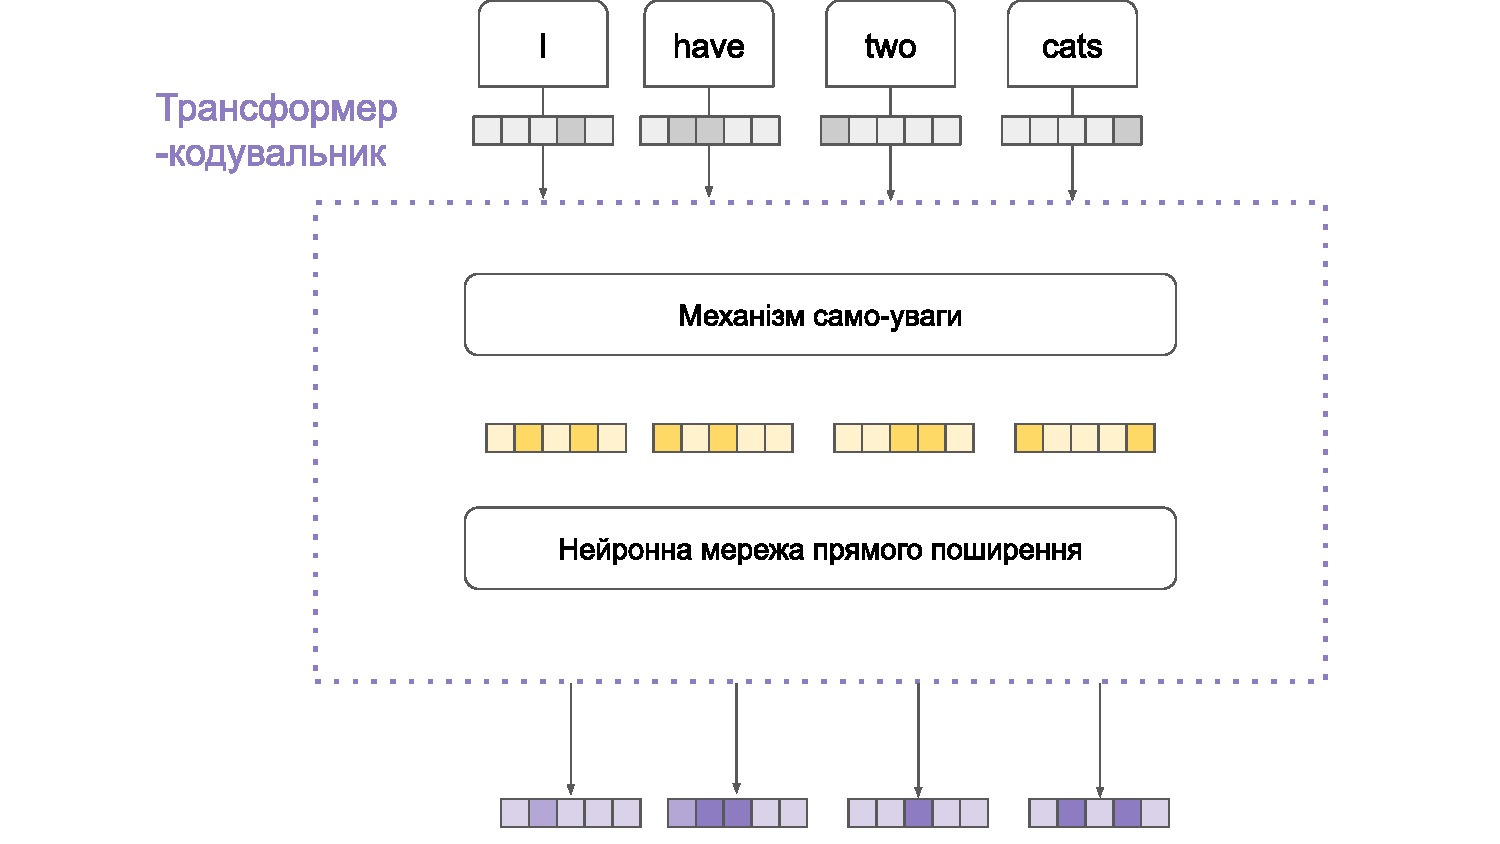
\includegraphics[width=0.9\textwidth]{encoder_block.pdf}
    \caption{Кодувальник моделі трансформер: механізм само-уваги + нейронна мережа прямого поширення.}
    \label{fig:encoder_block}
\end{figure}

Механізм само-уваги дозволяє моделі одночасно аналізувати всі позиції у вхідній послідовності за допомогою декодувальника, який має додатковий рівень уваги, що звертається до вихідних даних кодувальника.

Важливо, що у декодувальнику механізм само-уваги супроводжується маскуванням, щоб запобігати ``зазиранню у майбутнє''.

Наприклад, розглянемо наступне речення:
\begin{lstlisting}[language=json, breaklines=true]
I have two cats, they are fluffy.
\end{lstlisting}

У цьому випадку займенник ``they'' має відношення до слів ``cats'' та ``fluffy''. За допомогою механізму само-уваги модель обчислює вагові коефіцієнти між ``they'' та всіма іншими словами, визначаючи, що саме визначені слова мають найбільше відношення до виділеного слова. На рис.~\ref{fig:self_attention_visualisation} можна бачити взаємозв’язок між токеном ``they'' та рештою токенів у заданому реченні.

% https://colab.research.google.com/drive/1773-ssYunT6oi7vy6hhwwWzj3ibV_Ia5?authuser=1#scrollTo=twSVFOM9SopW
\begin{figure}[h]
    \centering
    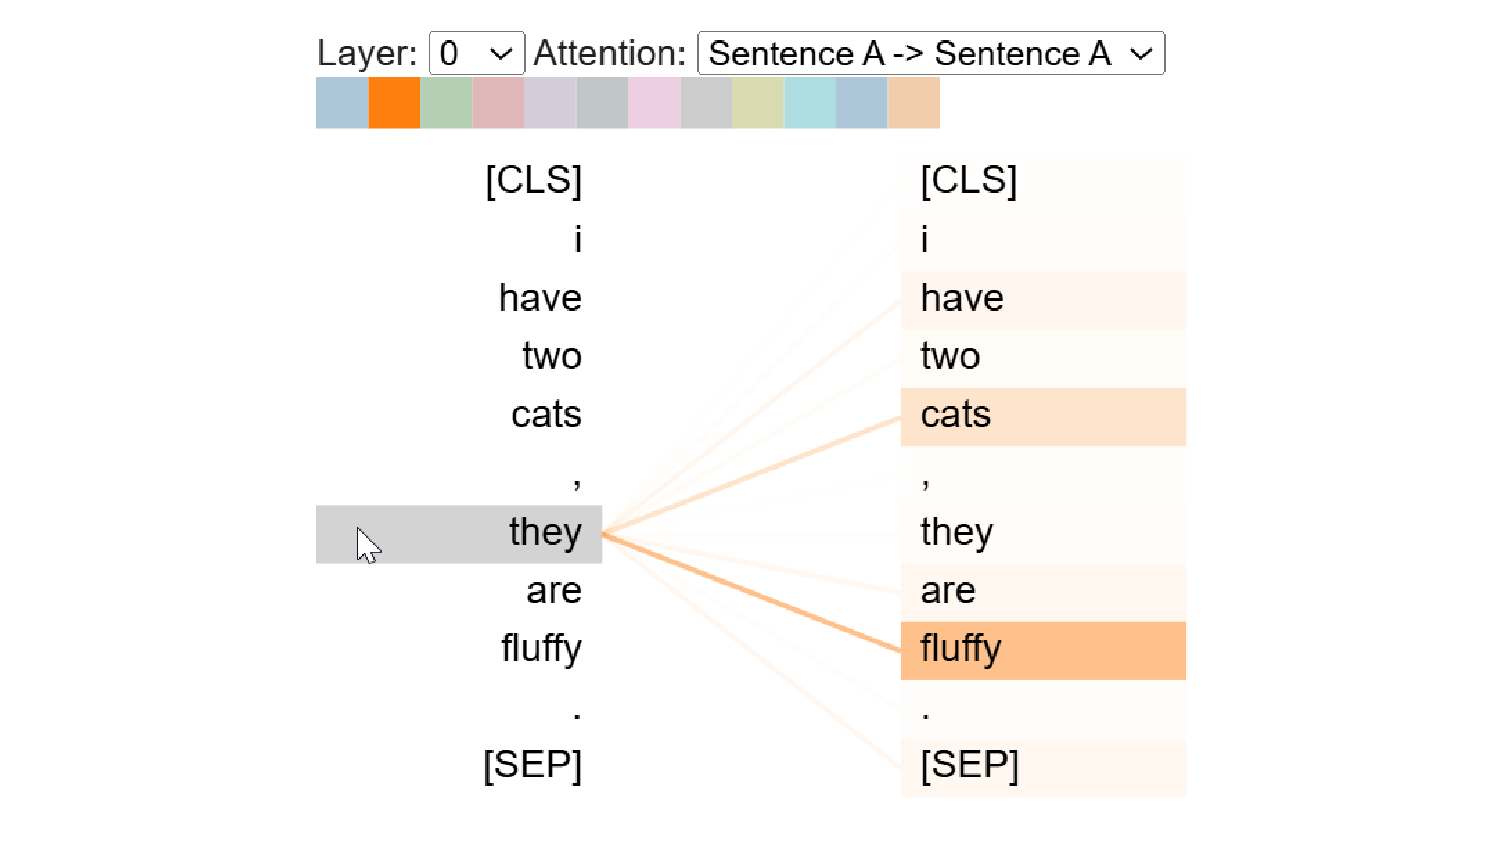
\includegraphics[width=0.6\textwidth]{self_attention_visualisation.pdf}
    \caption{Приклад зв'язків у реченні між токенами за допомогою механізму само-уваги.}
    \label{fig:self_attention_visualisation}
\end{figure}

Слід звернути увагу, що вхід містить додаткові спеціальні токени \texttt{[CLS]} (класифікаційний токен на початку тексту) та \texttt{[SEP]} (токен для ідентифікації кінця речення), які допомагають моделі ефективно обробляти вхідні речення та створювати відповідні представлення. Дані токени також зазвичай використовуються під час тонкого налаштування моделей на конкретних завданнях, таких як класифікація, аналіз тексту та семантичний пошук.

Архітектури, що базуються на моделі трансформер, утворюють основу двох фундаментальних категорій мовних моделей.

\paragraph{Моделі представлення}
Однією з моделей представлення (encoder-only models) є Pre-training of Deep Bidirectional Transformer (BERT) \cite{devlin2019bertpretrainingdeepbidirectional}. Ця модель використовує виключно кодувальні блоки, що складаються з механізму самоуваги та згорткових нейронних мереж, для формування семантичних представлень тексту. Приклад обробки речення за допомогою моделі BERT представлено на рис.~\ref{fig:bert_architecture}.

Додатково для проведення попереднього навчання, використовується крок -- \emph{масковане мовне моделювання (masked language modeling)}, який дозволяє моделі формувати двосторонні представлення, які потім адаптуються для конкретних завдань.

\begin{figure}[h]
    \centering
    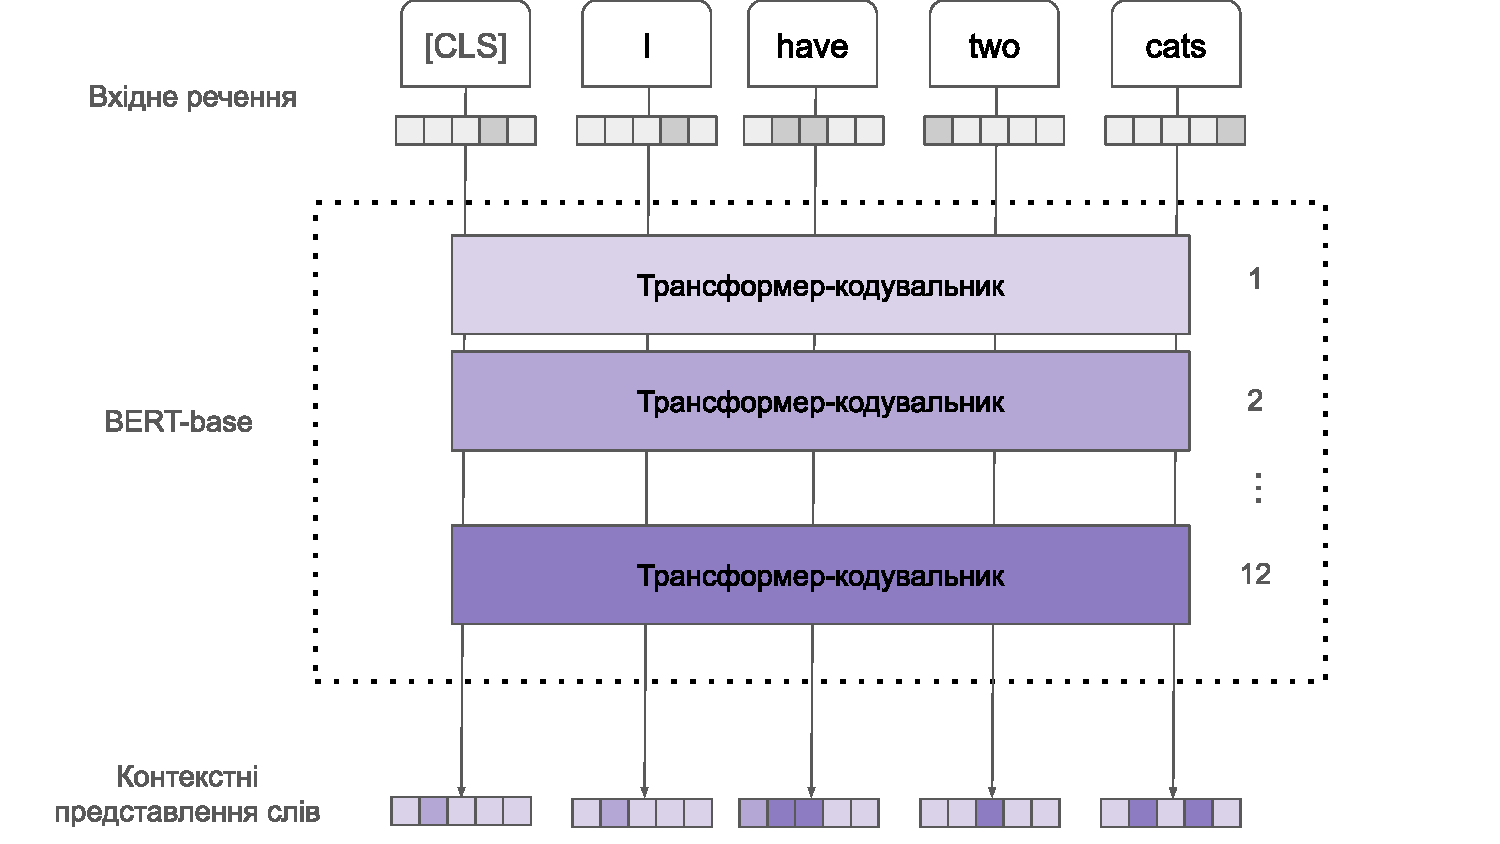
\includegraphics[width=0.9\textwidth]{bert_architecture.pdf}
    \caption{Архітектура базової моделі BERT: 12 кодувальних блоків для генерації представлень.}
    \label{fig:bert_architecture}
\end{figure}

\paragraph{Генеративні моделі.}

Генеративні моделі (decoder-only models), однією з яких є модель генеративного попередньо навченого трансформера (Generative Pretrained Transformer, GPT) \cite{yenduri2023generativepretrainedtransformercomprehensive}. Дана модель оперує виключно за допомогою декодувальних блоків. Завдяки авторегресивному підходу, кожен наступний токен генерується на основі попередніх вхідних даних. Дані системи демонструють високу ефективність у задачах генерації тексту таких як наприклад, написати підсумок тексту, завершити речення, згенерувати відповідь на запитання і тд. Загальний приклад архітектури зображено на рис.~\ref{fig:gpt_architecture}.

\begin{figure}[h]
    \centering
    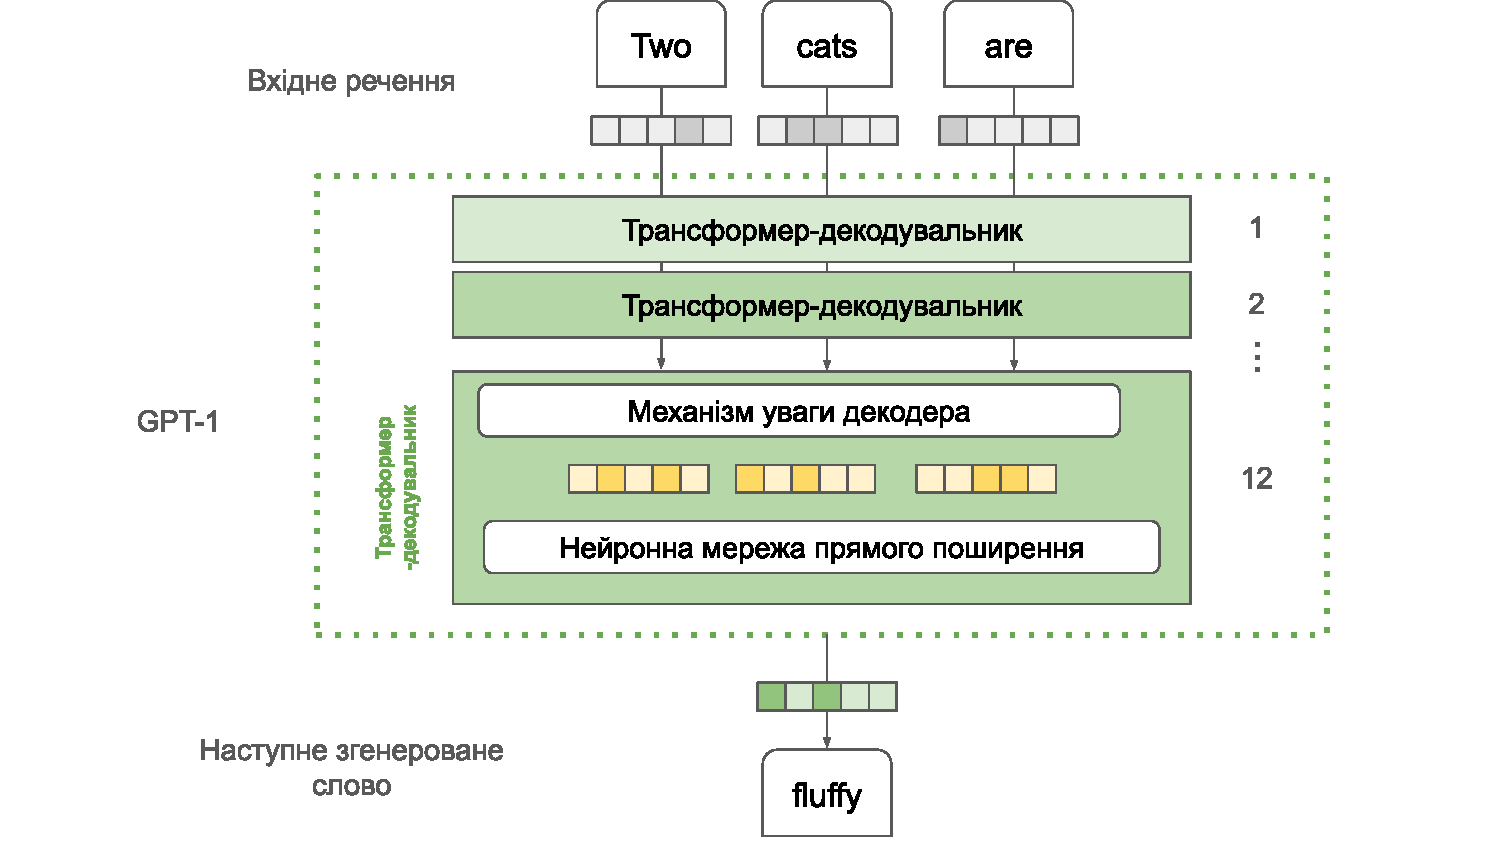
\includegraphics[width=0.9\textwidth]{gpt_architecture.pdf}
    \caption{Архітектура GPT-1: генеративна модель, що використовує лише декодувальник.}
    \label{fig:gpt_architecture}
\end{figure}

На практиці обидва типи моделей (генеративні моделі та моделі представлення) належать до категорії \emph{великих мовних моделей (large language models)}.

Важливою частиною цих моделей завершення є довжина контексту або \emph{контекстне вікно (context window)}. Довжина контексту представляє максимальну кількість токенів, яку модель може обробити, як показано на  рис.~\ref{fig:context_length}. Велике контекстне вікно дозволяє передавати до ВММ на вхід великі об'єми текстових даних. За рахунок авторегресивного підходу роботи цих моделей, поточна довжина контексту під час генерації нових токенів буде збільшуватися. У великих мовних моделях максимальна кількість контекстного вікна обмежується певною кількість токенів, які зазначаються у описі відповідних моделей.

\begin{figure}[h]
    \centering
    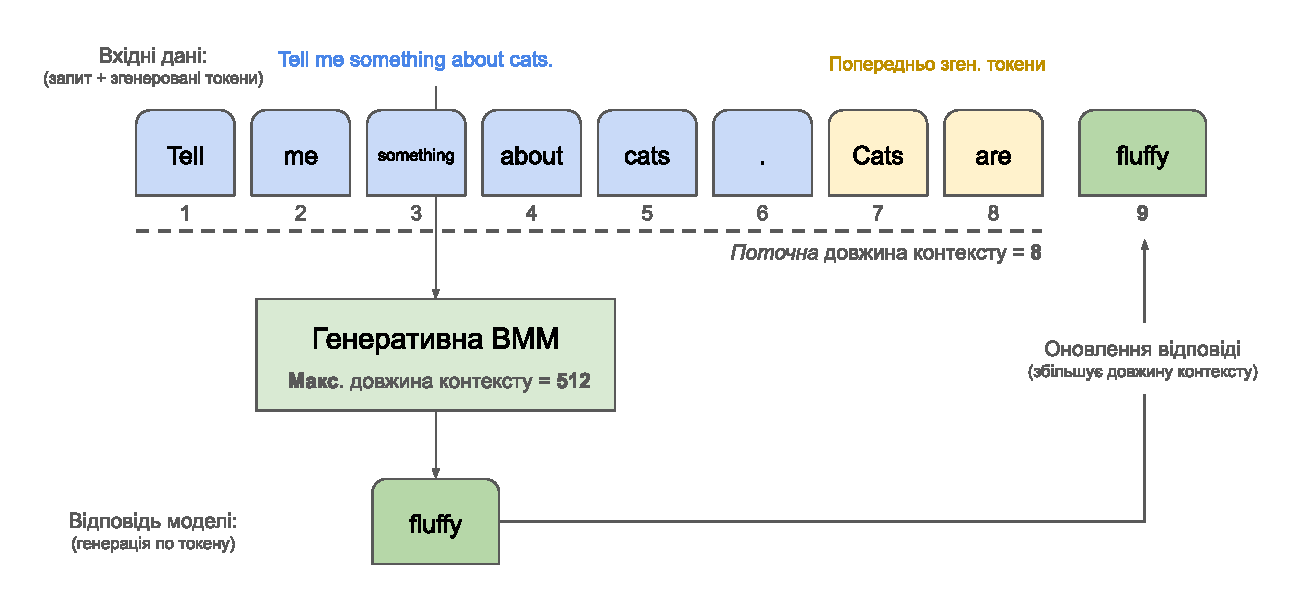
\includegraphics[width=0.9\textwidth]{context_length.pdf}
    \caption{Довжина контекстного вікна -- це максимальна довжина вхідних даних (у токенах), яка може бути оброблена моделлю.}
    \label{fig:context_length}
\end{figure}

%%%%%%%%%%%%%%%%%%%%%%%%%%%%%%%%%%%%%%%%%%%%%%%%%%%%%%%%%%%%%%%%%%%%%%%%%%%%%%
\subsection{Великі мовні моделі}

\paragraph{Парадигма тренування великих мовних моделей}

\begin{figure}[h]
    \centering
    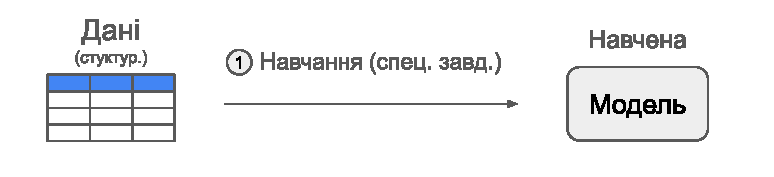
\includegraphics[width=0.6\textwidth]{ml.pdf}
    \caption{Традиційне машинне навчання включає один крок: навчання моделі для конкретного цільового завдання, наприклад, класифікації чи регресії.}
    \label{fig:ml}
\end{figure}

На відміну від традиційних методів машинного навчання, що базуються на навчанні моделей для виконання певного завдання -- рис.~\ref{fig:ml}, розробка ВММ передбачає багатоступеневий підхід. 
\begin{figure}[h]
    \centering
    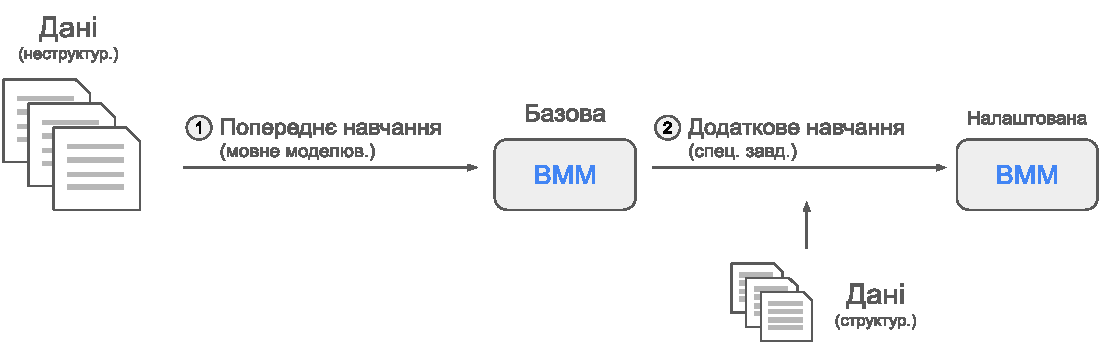
\includegraphics[width=0.9\textwidth]{llm_training.pdf}
    \caption{Багатокроковий процес навчання ВММ: попереднього тренування та тонкого налаштування.}
    \label{fig:llm_training}
\end{figure}

Як можна бачити з рис.~\ref{fig:llm_training}, типовий процес навчання сучасних трансформерних ВММ \cite{ouyang2022traininglanguagemodelsfollow} складається з трьох основних етапів:

\begin{enumerate}

    \item {Попереднє тренування (Pre-training)}
    На цьому етапі ВММ тренуються на великих корпусах текстів, щоб засвоїти загальні закономірності мови, граматику, семантичні зв’язки між елементами тексту з урахуванням особливостей відповідного завдання. Отримана ``базова'' модель є вихідною точкою для подальшої адаптації та удосконалення моделі на відповідних задачах. За рахунок попереднього тренування моделі вчаться прогнозувати наступний токен по заданому вхідному тексті. На рис.~\ref{fig:pretraining} зображено процес попереднього тренування моделі на корпусі даних Common Crawl.
    
    \item {Тонке налаштування (Fine-tuning)}
    На цьому етапі базову модель далі адаптують для виконання вузько-направлених завдань (класифікація, інформаційний пошук, генерація діалогів тощо), що дозволяє значно знизити обчислювальну вартість. Цей підхід, представлений на \ref{fig:llm_training}, є стандартним у сучасних методах розробки ВММ. Одним з різновидів додаткового навчання є кероване навчання (supervised fine-tuning), при якому моделі додатково навчаються на парах інструкція-відповідь, щоб покращити виконання спеціалізованих завдань.
    
    \item {Вирівнювання (Alignment)}: Додатковим етапом сучасних мовних моделей також є етап вирівнювання, під час якого моделі налаштовуються для більш корисних та безпечних відповідей на основі людського зворотного зв'язку. Задля цього використовуються такі методи як RLHF, про які буде розповідатися детальніше у одному з наступних розділів.
    
\end{enumerate}

% джерело: https://cameronrwolfe.substack.com/p/language-models-gpt-and-gpt-2
\begin{figure}[h]
\centering
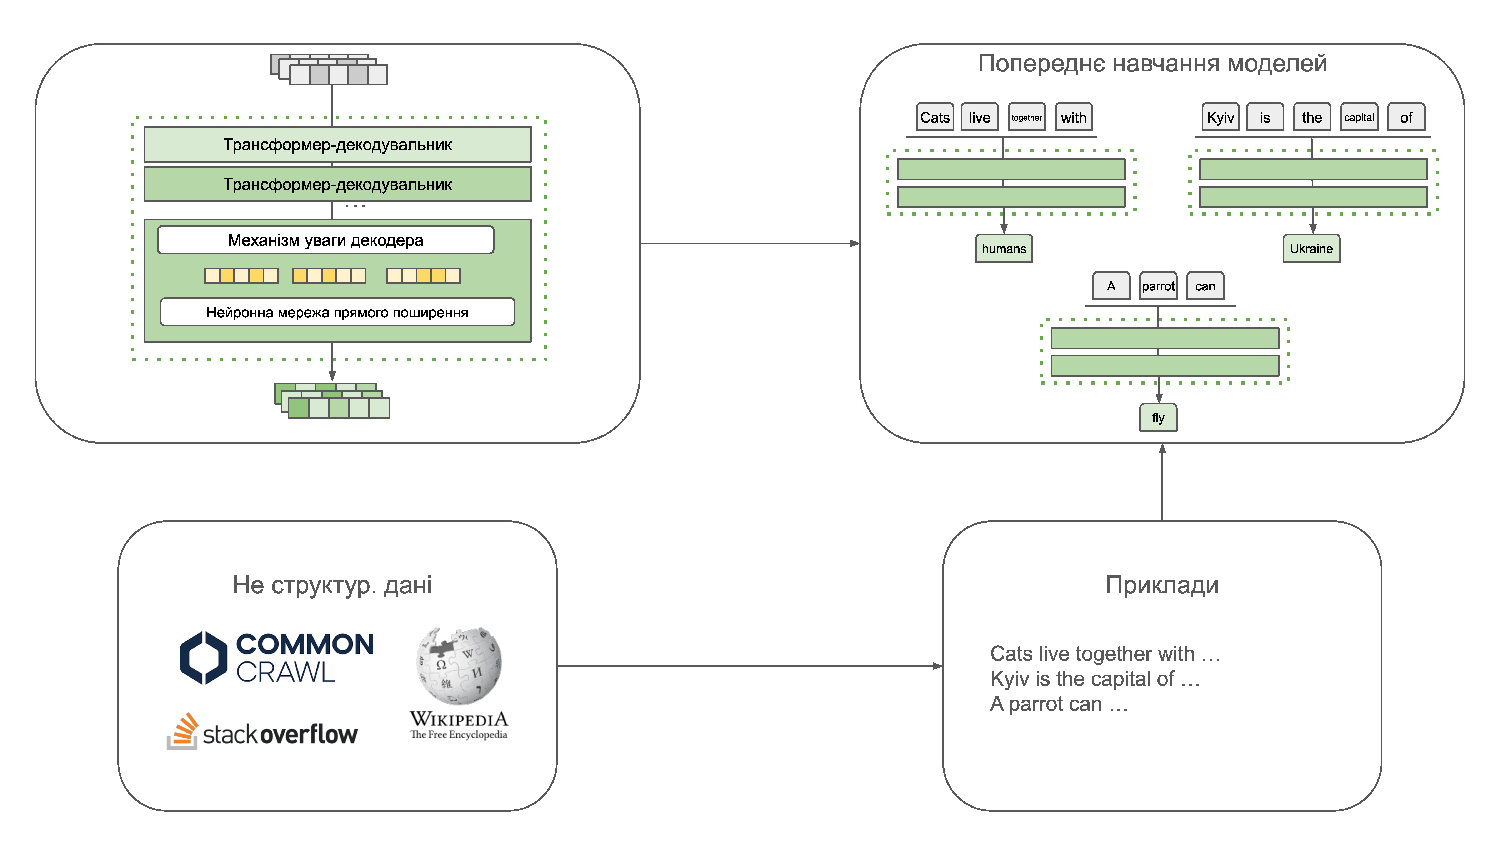
\includegraphics[width=0.9\textwidth]{llm_pretraining_step.pdf}
\caption{Ілюстрація етапу попереднього тренування ВММ.}
\label{fig:pretraining}
\end{figure}

\paragraph{Новітні тенденції та їх вплив на практику}
Останнім часом, особливо в 2022–2023 роках, технології на базі трансформерних моделей отримали значний вплив завдяки появі систем, що кардинально змінюють взаємодію користувачів з інформаційними технологіями. Швидке зростання активних користувачів, широке застосування мовного ШІ у різних галузях (від машинного перекладу до генерації контенту) сприяє подальшим інноваціям у цій сфері, а також вивченню етичних та соціальних наслідків впровадження таких технологій.

\paragraph{Застосування ВММ та соціально-етичні виклики.}

Великі мовні моделі мають застосування в багатьох галузях: від визначення тональності клієнтських відгуків (класифікація) до розробки інтерактивних чат-ботів, що використовують зовнішні інформаційні джерела для підвищення якості відповідей. Сучасні мультимодальні системи, зокрема генерація рецептів за зображенням вмісту холодильника, демонструють високий рівень інноваційності цих технологій.

Однак широке впровадження ВММ супроводжується й низкою соціально-етичних викликів. До них належать питання упередженості даних, проблеми прозорості алгоритмічних та архітектурних рішень, потенційна генерація шкідливого або дезінформаційного контенту, а також питання інтелектуальної власності. Врахування цих аспектів є необхідним для безпечного та відповідального використання технологій мовного ШІ.

ВММ, такі як GPT-4, демонструють значні здібності до розуміння та генерації математичних текстів, що відкриває можливості для їх використання у задачах математичного міркування \cite{openai2024gpt4technicalreport}.

Для подальшого удосконалення роботи ВММ з математичними текстами існує кілька методів, які наведені у наступному підрозділі.

%%%%%%%%%%%%%%%%%%%%%%%%%%%%%%%%%%%%%%%%%%%%%%%%%%%%%%%%%%%%%%%%%%%%%%%%%%%%%%
\section{Сучасні архітектури та методи для підвищення ефективності великих мовних моделей}

% https://huggingface.co/blog/moe
\subsection{Модель зі змішанням експертів}

Вперше ідея моделей зі змішанням експертів (MoE) була запропонована ще у 1991 році у роботі \textit{Adaptive Mixture of Local Experts} \cite{6797059}. Основна концепція MoE полягає в розбитті великої моделі на окремі моделі меншого розміру, яка отримали назву моделей-експертів або просто \emph{експертів (experts)}, кожен з яких спеціалізується на обробці певної підмножини завдань або видів вхідних даних. Вибір конкретного експерта або комбінації експертів здійснюється за допомогою спеціалізованого \emph{маршрутизатора (router)}, що визначає, яких із експертів активувати для обробки відповідного вхідного запиту.

У період між 2010-2015 роками архітектура з використанням MoE охоплювала два основних напрямки досліджень:
\begin{itemize}
    \item {Експерти як компоненти моделі}: Дані методи передбачали використання кількох незалежних моделей нейронних мереж, результати яких агрегувалися для отримання остаточного результату. Автори \cite{eigen2014learningfactoredrepresentationsdeep} пропонують інтеграцію MoE як окремого шару моделі, з використанням експертів, які спеціалізуються на обробці конкретних типів вхідних даних.
    \item {Умовні обчислення}: Традиційні щільні нейронні мережі (Dense Neural Networks) використовують всі параметри всіх шарів для обчислення результатів. Тому як більшу альтернативу \cite{bengio2016conditionalcomputationneuralnetworks} було запропоновано ефективне використання нейронної мережі, що дозволяє активувати лише певну підмножину параметрів залежно від особливостей вхідних даних. Таким чином, модель використовує лише частину параметрів нейронної мережі моделі, але при цьому має не гіршу та не рідко навіть кращу ефективність у порівнянні з моделями подібного розміру.
\end{itemize}

Загальний вигляд архітектури з використанням MoE-шару наведено на рис.~\ref{fig:moe-layer}.

\begin{figure}[!h]
    \centering
    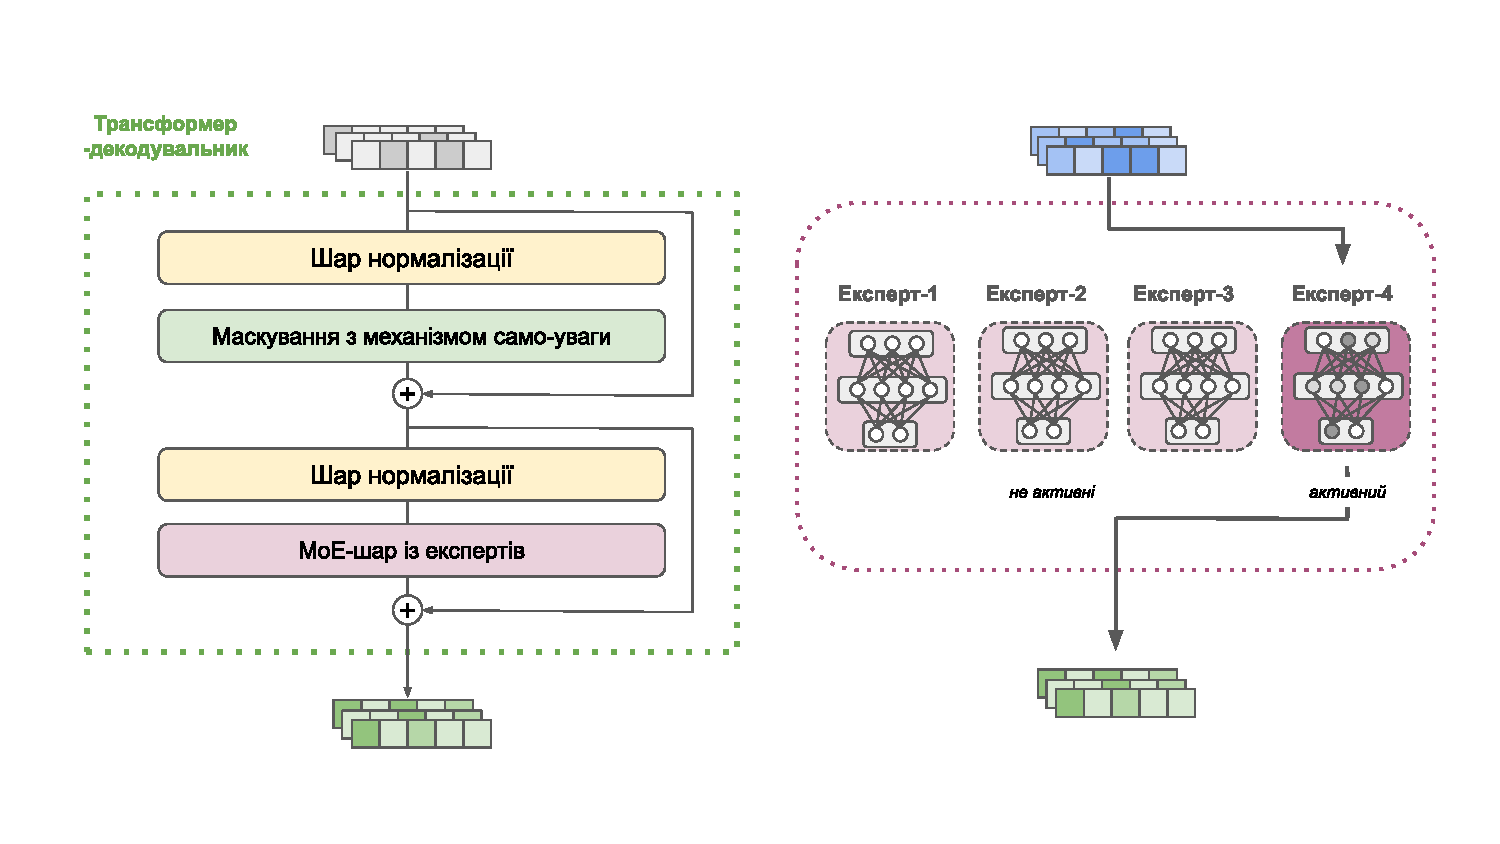
\includegraphics[width=0.9\textwidth]{moe_layer.pdf}
    \caption{MoE-шар моделі.}
    \label{fig:moe-layer}
\end{figure}

Після цього модель почали активно використовувати у задачах з NLP. Але спочатку визначимо поняття розрідженості (sparsity) у моделях.

\paragraph{Розрідженість у MoE}
Розрідженість моделей базується на ідеї використання умовних обчислень, при яких лише частина мережі активна в залежності від вхідних даних, що дозволяє збільшувати розмір моделі без збільшення обчислень, що дозволяє використовувати велику кількість експертів у кожному окремому шарі MoE.

Однак, ця конфігурацію створює певні виклики. Наприклад, якщо пакетний вхід складається з 10 токенів, п'ять токенів можуть потрапити до одного експерта, а інші п'ять -- до п'яти різних експертів, що призводить до нерівних розмірів розподілу вхідних даних.

Для вирішення цієї проблеми використовується навчена мережа маршрутизатор ($G$), яка вирішує, до яких експертів ($E$) відправити вхідний запит:

\begin{equation}
    y = \sum_{i=1}^{n} G(x)_i E_i(x)
\end{equation}

У даній конфігурації всі експерти запускаються для всіх входів. Якщо для деякого з експертів значення $G_i=0$, обчислення відповідного експерта не використовуються, і таким чином запобігається використання відповідних обчислювальних ресурсів. Зазвичай у якості функції активації мережі маршрутизатора використовується softmax. Мережа навчається визначати, до якого експерта відправити вхід:

\begin{equation}
    G_{\sigma}(x) = \text{Softmax}(x \cdot W_g)
\end{equation}

Інший підхід, який наприклад досліджувався у роботі \cite{shazeer2017outrageouslylargeneuralnetworks} -- Noisy Top-k Gating. Цей підхід вводить регульований шум і зберігає топ-$k$ значень:

Це робиться за рахунок додавання шуму:

\begin{equation}
    H(x)_i = (x \cdot W_g)_i + \text{StandardNormal()} \cdot \text{Softplus}((x \cdot W_{\text{noise}})_i)
\end{equation}

Після чого обираються лише топ-$k$ значення:

\begin{equation}
    \text{KeepTopK}(v, k)_i = \begin{cases}
        v_i, & \text{якщо } v_i \text{ входить до топ } k \text{ елементів } v, \\
        -\infty, & \text{інакше}
    \end{cases}
\end{equation}

І далі використовується softmax від отриманого результату:

\begin{equation}
    G(x) = \text{Softmax}(\text{KeepTopK}(H(x), k))
\end{equation}

Оскільки розрідженість керована параметром $k$, вона має додаткові особливі властивості. Використовуючи досить низьке $k$, можна тренувати та виконувати висновок набагато швидше, ніж при активації багатьох експертів. Маршрутизація до більше ніж одного експерта необхідна для того, щоб маршрутизатор навчився розподіляти вхідний запит між кількома експертами.

Додавання шуму сприяє балансуванню навантаження. Якщо всі токени надсилаються до лише декількох популярних експертів, тренування може призвести до нерівномірного тренування моделей. Це відбувається на етапі попереднього тренування MoE-моделі, коли маршрутизатор обирає схожих експертів за рахунок того, що обрані експерти тренуються швидше і тому вибираються частіше. Щоб уникнути цього, додається допоміжна функція втрат, яка заохочує рівномірний розподіл використання експертів. Ця функція втрат гарантує, що всі експерти отримують приблизно однакову кількість навчальних прикладів.

\paragraph{MoE та моделі трансформери}
У трансформерних моделях MoE застосовуються як шари, що замінюють звичайні шари щільних нейронних мереж прямого поширення. Структура такого шару MoE складається з двох основних компонентів:
\begin{enumerate}
    \item {Шарів експертів}: кожен експерт зазвичай реалізується у вигляді окремого шару FNN, що відповідає за обчислення для певної підмножини вхідних токенів. Структура експертів може відрізнятися, проте існують варіанти, коли експерти реалізуються як більш складні мережі або як набір експертів, що дозволяє моделі комплексно адаптуватися до різних типів даних.
    \item {Маршрутизатор}: цей компонент аналізує вхідний токен (або його представлення) і за допомогою функції softmax розраховує вагові коефіцієнти для кожного експерта. Таким чином, маршрутизатор вибирає топ-$k$ експертів (часто $k=1$ або $2$) для обробки даного токена. Такі підходи, як Noisy Top-$k$ Gating, вводять регульований шум для балансування навантаження між експертами та зниження надмірної спеціалізації окремих модулів.
\end{enumerate}

Завдяки даному підходу при обробці кожного вхідного прикладу активуються лише частина експертів, що дозволяє збільшувати модель до значно більшої кількості параметрів без активації усіх параметрів моделі. У зв'язку з цим такі моделі також називають розрідженими (sparse), адже при роботі моделей використовується лише частина параметрів.

\paragraph{Приклади моделей MoE}
Одним із прикладів застосування MoE у трансформерних моделях є Switch Transformers \cite{fedus2022switchtransformersscalingtrillion}. У цій моделі щільні FNN-шари звичайного трансформера замінюються розрідженими MoE-шарами. Кожен MoE-шар може складатися з декількох експертів, проте для кожного входу активується лише частина експертів, що значно знижує обчислювані навантаження під час генерації вихідних даних. Моделі даного типу дозволили досягнути чотирикратного прискорення попереднього тренування моделі у порівнянні зі щільними архітектурами, але при цьому зберігаючи високу якість результатів.

Іншим прикладом є система GShard \cite{lepikhin2020gshardscalinggiantmodels}, де розріджені MoE-шари інтегровані в трансформерну архітектуру для збільшення моделі до понад 600 мільярдів параметрів. У цій системі шари MoE розподіляються між різними пристроями, що дозволяє ефективно використовувати обчислювальні ресурси при обробці великих обсягів тренувальних даних.

Таким чином, інтеграція MoE в трансформерні архітектури має ряд важливих переваг:
\begin{itemize}
    \item {Ефективне збільшення моделей}: При збереженні однакових обчислювальних затрат розріджена модель MoE містить значно більше параметрів, ніж щільна модель, що дозволяє використовувати набагато більше даних і підвищувати якість попереднього тренування моделей.
    \item {Умовні обчислення}: Завдяки маршрутизатору активуються лише релевантні експерти для кожного вхідного запиту, що дозволяє зменшити обчислювальні витрати.
    \item {Спеціалізація експертів}: Кожен експерт може адаптуватися до обробки певних типів вхідних даних, що сприяє кращому моделюванню складних семантичних залежностей у відповідних даних.
\end{itemize}

Слід зазначити, що згідно із дослідженнями у використанні архітектури MoE у моделях (наприклад, \cite{xue2024openmoeearlyeffortopen}) різні експерти не спеціалізуються на конкретних темах, таких як біологія, математика тощо. Проте працюють з певними наборами токенів, які подаються на вхід моделей. Як результат -- моделі схильні категоризувати роботу з певними природними мовами (наприклад, англійська, українська), адже вони несуть свої особливості у символьному представленні слів. Орієнтованість на вибір відповідних задач можна бачити при перегляді найбільш активно вживаних токенів відповідними експертами, як наведено у таблиці~\ref{tab:top_token_table}.

\begin{figure}[h]
    \centering
    \captionof{table}{Найчастіше вживані токени, що використовуються різними експертами \cite{xue2024openmoeearlyeffortopen}.}
    \label{tab:top_token_table}
    \begin{tabular}{|c|l|}
        \hline
        ID експерта & Найбільш активно вживані токени \\
        \hline
        0 & \hlblue{\textbackslash n}, \hlblue{`}, \hlblue{’}, \hlblue{s}, \hlblue{-}, \hlblue{\$}, \hlblue{y}, \hlblue{\_}, \hlblue{\,}, \hlblue{2} \\
        1 & \hlgreen{\textbackslash n}, \hlgreen{1}, \hlgreen{\,}, \hlgreen{2}, \hlgreen{\textbackslash\textbackslash}, \hlgreen{S}, \hlgreen{.}, \hlgreen{-}, \hlgreen{C}, \hlgreen{\{} \\
        21 & \hlred{,}, \hlred{and}, \hlred{\,}, \hlred{.}, \hlred{\textbackslash n}, \hlred{=}, \hlred{\textbackslash t}, \hlred{the}, \hlred{\,}, \hlred{n} \\
        30 & \hlpurple{\}}, \hlpurple{ed}, \hlpurple{d}, \hlpurple{have}, \hlpurple{ing}, \hlpurple{,}, \hlpurple{has}, \hlpurple{s}, \hlpurple{\"}, \hlpurple{had} \\
        31 & \hlgrey{to}, \hlgrey{can}, \hlgrey{s}, \hlgrey{of}, \hlgrey{ing}, \hlgrey{will}, \hlgrey{not}, \hlgrey{e}, \hlgrey{ed}, \hlgrey{would} \\
        \hline
    \end{tabular}
\end{figure}


Однак, моделі зі змішанням експертів мають свої недоліки, зокрема:
\begin{itemize}
    \item {Балансування навантаження}: Одні експерти можуть активуватися частіше, що призводить до нерівномірного розподілу обчислювальних ресурсів та їхнього потенційного перенавчання (overfitting).
    \item {Супутні обчислювальні та комунікаційні витрати}: Хоча під час висновку активуються лише обрані експерти, всі параметри повинні бути завантажені в оперативну пам’ять, що може створювати додаткові вимоги до апаратного забезпечення.
\end{itemize}

Щоб вирішити ці проблеми, застосовуються такі методи, як додавання надмірного шуму до маршрутизатора та додаткові функції втрат (loss function), які стимулюють рівномірний розподіл навантаження між моделями-експертами. Також застосовуються методи умовної маршрутизації, що дозволяють ефективно задіювати обчислювальний ресурс при навчанні та генерації відповідей.

У підсумку, MoE представляють собою потужний підхід для збільшення параметрів трансформерних архітектур із збереженням обчислювальної ефективності та високої якості моделі. Нижче наведені деякі приклади моделей, які ілюструють практичне застосування цієї ідеї в сучасних системах обробки природної мови та їх порівняння з традиційними моделями, що використовують щільні нейронні мережі.

\paragraph{Приклади моделей з використанням MoE}
Після обґрунтування концепції MoE, розглянемо кілька прикладів даних моделей. Завдяки тому, що великі мовні моделі збільшують ефективність своєї роботи при збільшенні параметрів, MoE були широко впроваджені і досягли успіху у дослідженнях з ВММ.

Одним з прикладім моделей з використанням MoE є Mixtral 8×7B (Mixtral of Experts \cite{jiang2024mixtralexperts}) та є розширенням для відкритої моделі Mistral-7B \cite{jiang2023mistral7b}, яка володіє англійською, французькою, італійською, німецькою та іспанською мовами. Обидві ці моделі мають оприлюднені ваги та інші специфікації задля відкритого користування розробниками та дослідниками.

\begin{figure}[h]
    \centering
    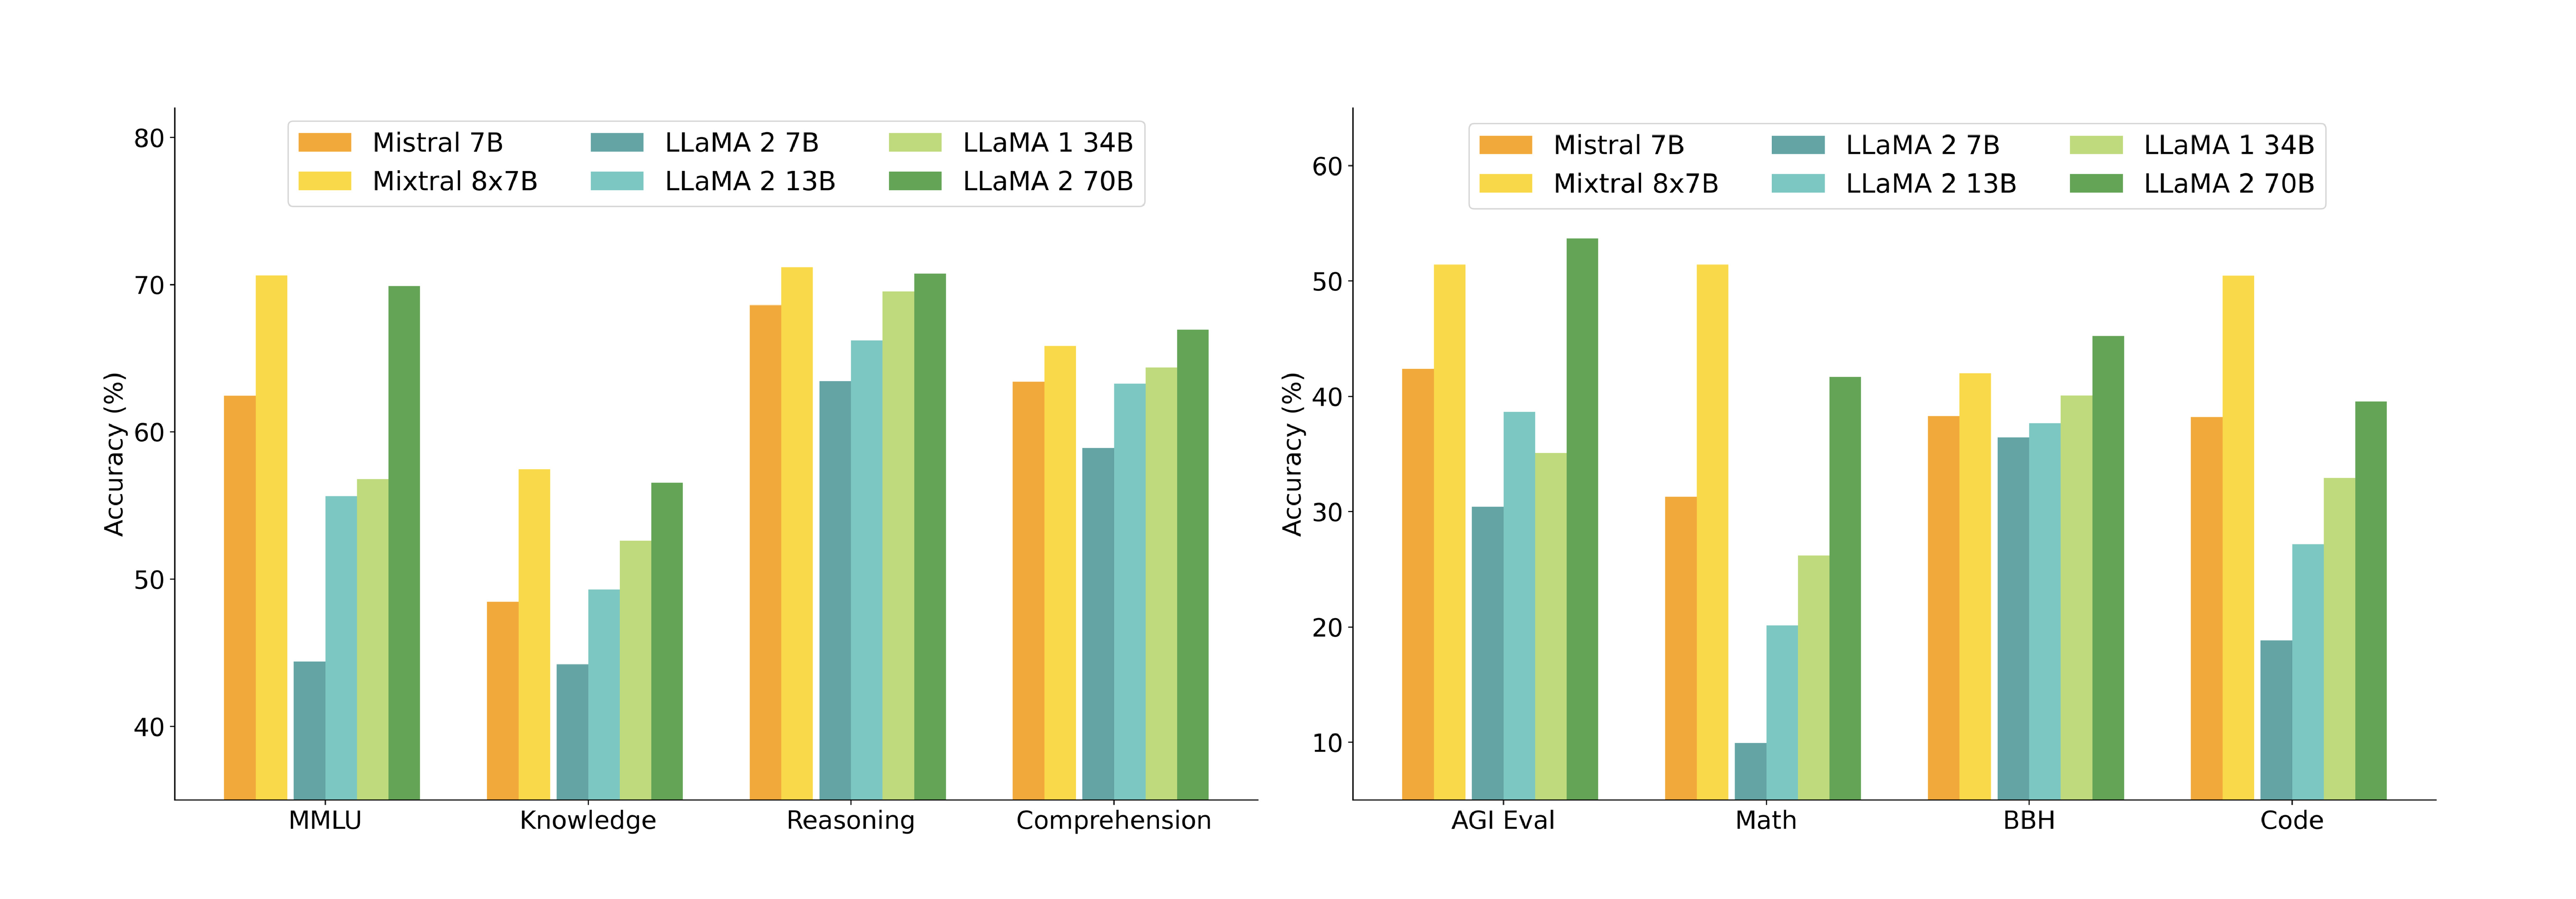
\includegraphics[width=1.0\textwidth]{llama2-v-mistral.pdf}
    \caption{Порівняння роботи моделі з MoE-шаром (Mixtral) прости моделі з FNN-шаром (LLaMA 2) \cite{jiang2024mixtralexperts}.}
    \label{fig:llama2-v-mistral}
\end{figure}

Mixtral перетворює кожен шар Mistral на експертний шар з вісьмома експертами. Для кожного вхідного токена активні два експерти, що робить модель із 47 млрд. загальними параметрами використовувати лише 13 млрд. активних параметрів. Модель також має довжину контекстного вікна у 32 тис. токенів, що у 4 рази більша, ніж у її аналога без MoE. Як показано на представленому рис.~\ref{fig:llama2-v-mistral}, Mixtral перевершує суміжну по кількості параметрів модель LLaMA 2 за всіма показниками та особливо виділяється у генерації програмного коду, математичних завданнях та інших метриках, в деяких випадках перевищуючи ефективність більшої моделі LLaMA-2-70B \cite{touvron2023llama2openfoundation}.

% % %  Chain-Of-Thought
% https://www.promptingguide.ai/techniques/cot
\subsection{Ланцюг міркування}

\paragraph{Інженерія запитів} Сучасні великі мовні моделі, такі як GPT-3.5 Turbo, GPT-4 та Claude 3, налаштовані на виконання інструкцій та треновані на великих обсягах даних. Це дозволяє даним моделям виконувати деякі завдання у режимі питання-відповідь без або з додатковою демонстрацією бажаного вихідного результату. Набір технік направлений на тестування моделей за відповідними підходами називають інженерією запитів (Prompt Engineering), а вхідну інструкцію запитом (prompt).

Інженерія запитів -- це процес розробки, оптимізації та адаптації текстових запитів, що використовуються для взаємодії з мовними моделями з метою досягнення бажаних результатів. Цей підхід охоплює формулювання запитів, визначення формату відповіді та забезпечення коректної інтерпретації інструкцій моделлю.

Оскільки моделі є генеративними, вони здатні виконувати різноманітні запити -- від генерації есе до відповідей на математичні запитання. Нижче наведено приклад запиту:

\begin{lstlisting}[language=json, breaklines=true]
{"content": "Solve the following math problem and justify your answer:
            You want to arrange 10 apples between 2 baskets.
            One basket must contain twice as many apples as another one.
            How many apples should be in each basket? Give a short answer."}
\end{lstlisting}

\paragraph{Підходи Zero-shot і Few-shot.}
Розрізняють кілька підходів до інженерії запитів при роботі з великими мовними моделями.

\emph{Zero-shot} -- це режим взаємодії з мовною моделлю, коли для виконання задачі використовується запит, що не містить жодних прикладів або демонстрацій потрібної поведінки. Модель повинна інтерпретувати завдання виключно з опису запиту.

\emph{Few-shot} -- це режим, при якому до запиту додаються декілька прикладів (демонстрацій), що ілюструють очікувану поведінку. Завдяки таким прикладам мовна модель отримує краще розуміння специфіки або особливостей завдання, що робить процес генерації відповіді більш релевантним до завдання.

\paragraph{Ланцюг мислення}
Задля забезпечення точності роботи мовних моделей було запропоновано \emph{метод ланцюга міркувань (Chain-of-Thought, CoT)}, що дозволяє моделям генерувати послідовність міркувань, які покращують їхню здатність до розв'язання складних задач. Метод ланцюжка міркувань дозволяє моделям генерувати проміжні кроки міркувань, що покращує їхню здатність до розв'язання задач без додаткового навчання на спеціалізованих даних \cite{kojima2023largelanguagemodelszeroshot}.
Вперше ланцюг міркування був представлений у роботі \cite{wei2023chainofthoughtpromptingelicitsreasoning} і дозволяє моделям здійснювати складне міркування за допомогою проміжних кроків. 

\begin{figure}
    \centering
    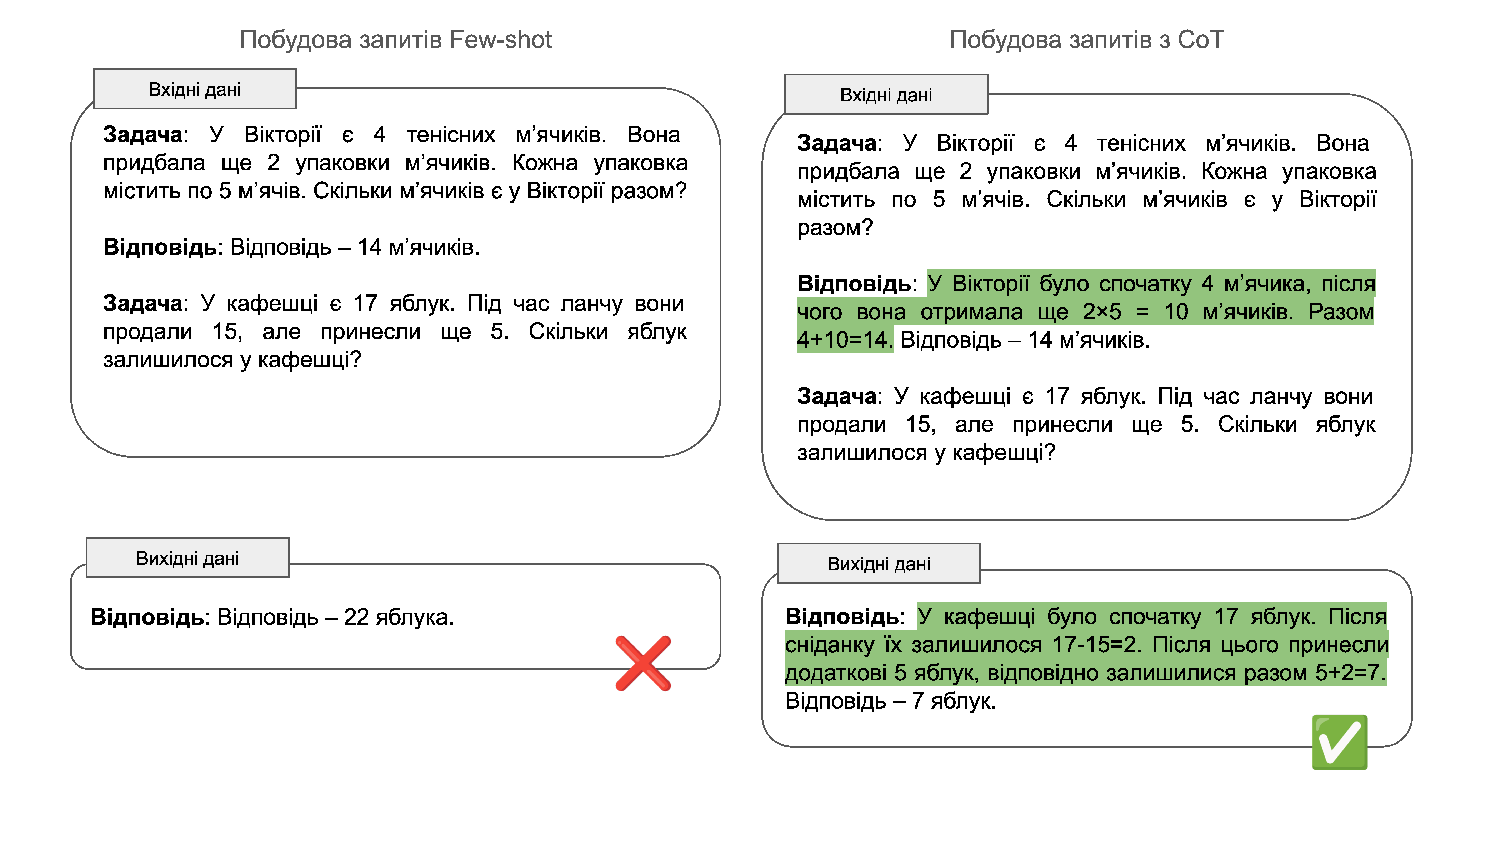
\includegraphics[width=1\textwidth]{cot.pdf}
    \caption{Приклад використання техніки CoT у інженерії запитів.}
    \label{fig:cot}
\end{figure}

Цей метод можна поєднувати з Few-shot навчанням для досягнення кращих результатів у більш складних завданнях, що потребують роздумів перед відповіддю. Загальний приклад використання ланцюга міркувань можна бачити на рис.~\ref{fig:cot}.

Приклад використання CoT при розв'язанні задачі за допомогою мовної моделі продемонстровано у таблиці.~\ref{tab:train_distance}.

\begin{figure}[h]
    \centering
    \small
    \captionof{table}{Приклад ланцюжка думок у задачі для розрахунку відстані, яку пройде потяг.}
    \label{tab:train_distance}
    \begin{tabular}{|l|p{10cm}|}
        \hline
        \textbf{Етап міркування} & \textbf{Опис} \\
        \hline
        \textbf{Питання} & Приблизна відстань між Києвом та Полтавою - 340 км. Потяг рухається із середню швидкістю 85 км./год. За скільки годин потяг пройде дану відстань? \\
        \hline
        \textbf{Крок 1} & Визначення даних: швидкість - 85 км/год, відстань - 340 км. \\
        \hline
        \textbf{Крок 2} & Формула відстані: \[ t = \dfrac{S}{\upsilon} \] \\
        \hline
        \textbf{Крок 3} & Розрахунок - час на проходження відстані: \[ t = \dfrac{340}{85} = 4 \text{ год.}\] \\
        \hline
        \textbf{Розв'язок} & Потяг добереться з Києва до Полтави за 4 год. \\
        \hline
    \end{tabular}
\end{figure}

Подібні приклади демонструють, як ланцюг міркувань допомагає моделі аналізувати та робити обґрунтовані висновки. Навіть з одним прикладом, модель може ефективно вирішувати подібні завдання.

\paragraph{Zero-shot CoT}
Одним з останніх підходів для інженерії запитів є Zero-shot CoT, який було запропонована у роботі \cite{kojima2023largelanguagemodelszeroshot}. Вона передбачає додавання фрази ``Давайте поміркуємо крок за кроком'' (``Let's think step-by-step'') до початкового запиту як на рис.~\ref{fig:zero_cot}.

\begin{figure}
    \centering
    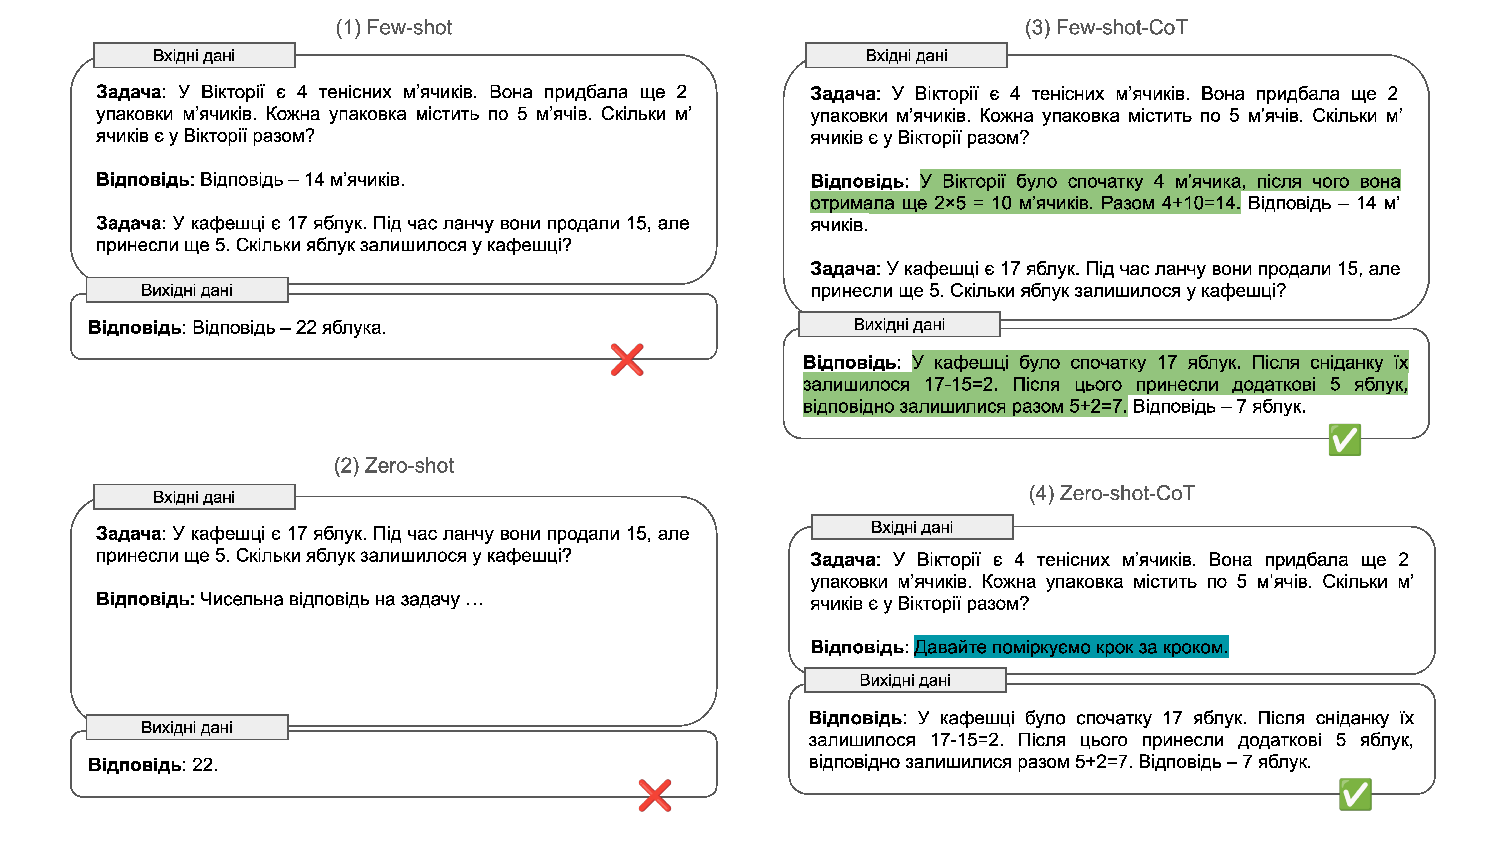
\includegraphics[width=1\textwidth]{zero-cot.pdf}
    \caption{Приклад використання техніки Zero-shot CoT.}
    \label{fig:zero_cot}
\end{figure}

Цей підхід є ефективним, особливо у випадках, коли немає достатньо великої кількості прикладів для демонстрації очікуваної роботи.

\paragraph{Auto-CoT}
При застосуванні CoT з демонстраціями необхідно вручну створювати ефективні та різноманітні запити, що не завжди є можливим та оптимальним рішенням. \cite{zhang2022automaticchainthoughtprompting} запропонували підхід Auto-CoT, який автоматично генерує ланцюги міркувань.

Метод Auto-CoT складається з двох основних етапів:
\begin{enumerate}
    \item {Кластеризація запитань:} Розподіл запитань певного набору даних на кілька кластерів.
    \item {Вибір демонстрацій:} Вибір представницького запитання з кожного кластеру та генерація його ланцюга міркувань за допомогою Zero-Shot CoT з додатковими евристиками.
\end{enumerate}

Цей метод сприяє створенню простих і точних запитів, зменшуючи ризик помилок у згенерованих ланцюгах міркувань моделлю.

\subsection{Навчання з підкріпленням з людським зворотнім зв'язком}

Сучасні великі мовні моделі, як наприклад LLaMA, використовують метод навчання з підкріпленням з людським зворотним зв'язком (Reinforcement Learning with Human Feedback, RLHF) як невід'ємну частину свого навчального процесу. RLHF дозволяє інтегрувати зворотній зв'язок від людини у процес оптимізації моделі, що покращує її корисність та безпечність. У цьому підрозділі розглядається метод RLHF, його роль у навчанні ВММ та альтернативні методи до тонкого налаштування (fine-tuning) моделей.

Традиційний метод RLHF, описаний у роботі InstructGPT \cite{ouyang2022traininglanguagemodelsfollow}, складається з трьох основних кроків:

\begin{figure}[h]
    \centering
    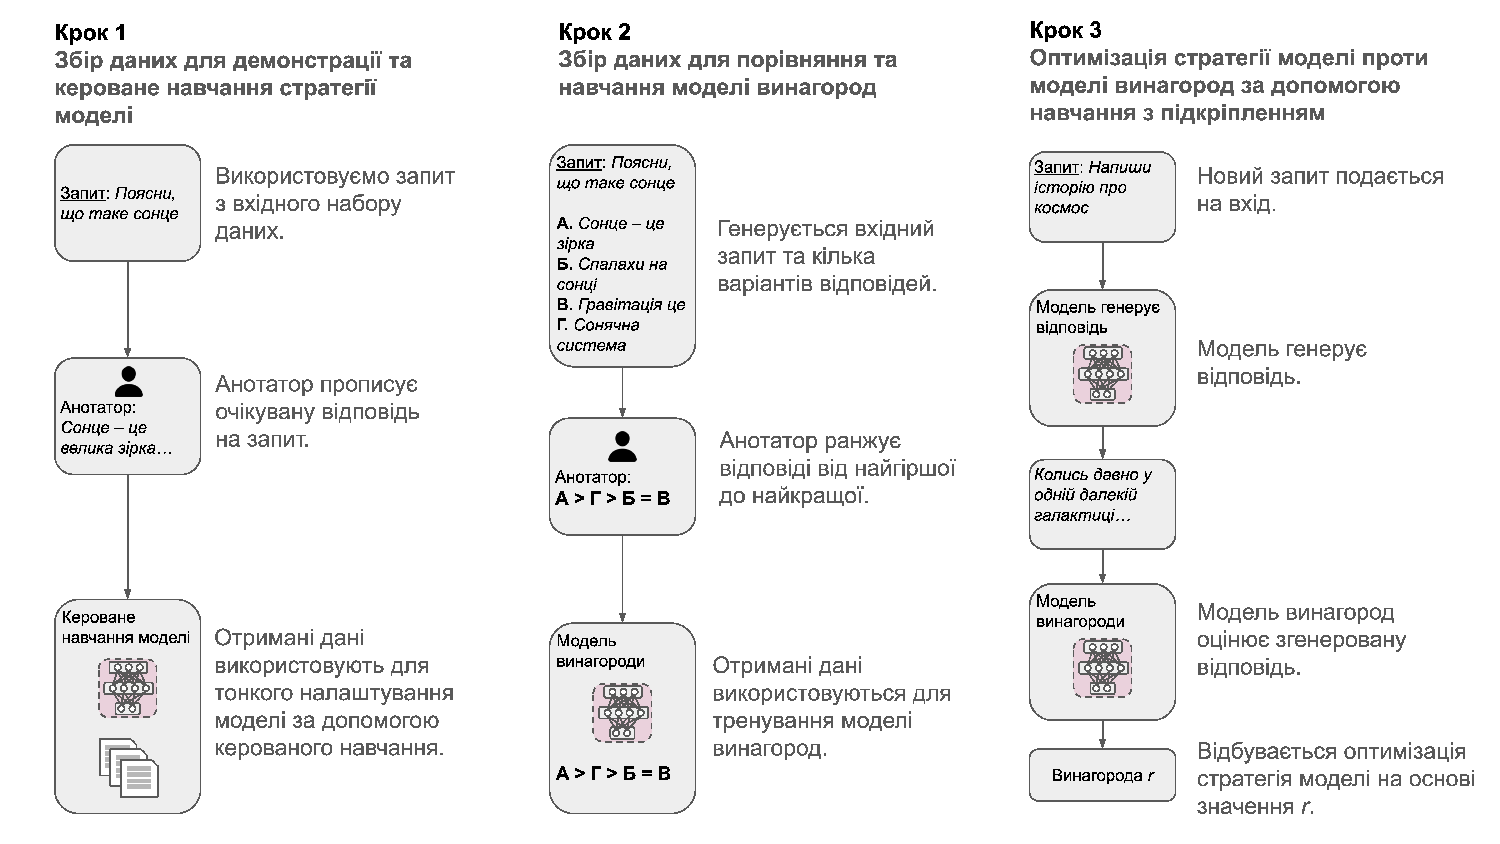
\includegraphics[width=1.0\textwidth]{rlhf.pdf}
    \caption{Тонке налаштування моделі на основі методу RLFH.}
    \label{fig:rlhf}
\end{figure}

\paragraph{Крок 1: Збір даних для демонстрації та кероване навчання стратегії моделі}
На першому кроці рис.~\ref{fig:rlhf} показано етап керованого навчання, де модель навчається на парах інструкція-відповідь, створених людьми-анотаторами. Цей етап покращує здатність моделі слідувати конкретним інструкціям.

\paragraph{Крок 2: Збір даних для порівняння та навчання моделі винагород}
Як показано на другому кроці рис.~\ref{fig:rlhf}, для кожної інструкції генеруються декілька відповідей за допомогою моделі з кроку 1. Анотатори ранжують ці відповіді за уподобаннями. На основі цих ранжувань навчається модель винагород (reward model), яка оцінює якість згенерованих відповідей.

\paragraph{Крок 3: Оптимізація стратегії моделі проти моделі винагород за допомогою навчання з підкріпленням}
На третьому кроці з рис.~\ref{fig:rlhf} зображено процес оптимізації моделі із використанням методу Proximal Policy Optimization (PPO) \cite{schulman2017proximalpolicyoptimizationalgorithms}, де модель покращує стратегію роботи за рахунок оцінки від моделі винагород.

\subsubsection{RLHF у моделі LLaMA 2}

У моделі LLaMA 2 від Meta AI також використовується RLHF, але з деякими відмінностями від методу описаного у InstructGPT \cite{touvron2023llama2openfoundation}. Модель містить 3 особливості:
\begin{enumerate}
    \item {Дві моделі винагород.} LLaMA 2 використовує дві окремі моделі винагород: одну для оцінки корисності, іншу -- для безпеки. Загальна винагорода є лінійною комбінацією цих двох оцінок, що дозволяє збалансувати ці аспекти при донавчанні моделі.
    \item {Метод відбору проб.} Крім PPO, у LLaMA 2 використовується метод відбору проб (rejection sampling) для відбору найкращих відповідей з кількох згенерованих варіантів на кожному кроці навчання. Це покращує ефективність навчання, оскільки модель навчається на відповідях з вищою оцінкою винагороди. Використовується для відбору відповідей з найвищою винагородою з декількох згенерованих варіантів \cite{ziegler2020finetuninglanguagemodelshuman}. На рис.~\ref{fig:llama2_performance} представлено покращення моделі LLaMA 2 на різних етапах RLHF, де видно, що використання PPO в кінцевому етапі призводить до кращих результатів.
    Загалом, RLHF є потужним інструментом для тонкого налаштування великих мовних моделей, дозволяючи інтегрувати людський зворотній зв'язок та підвищити якість відповідей.
    \item {Функція розділення втрати.} На відміну від методу у InstructGPT, де використовувався між-ентропійна функція втрат для ранжування відповідей, у моделі LLaMA 2 впроваджено додатковий параметр функції розділення втрат (margin loss). Цей параметр дозволяє враховувати ступінь переваги однієї відповіді над іншою, що сприяє більш якісному донавчанні моделі винагород.
\end{enumerate}

\begin{figure}[h]
    \centering
    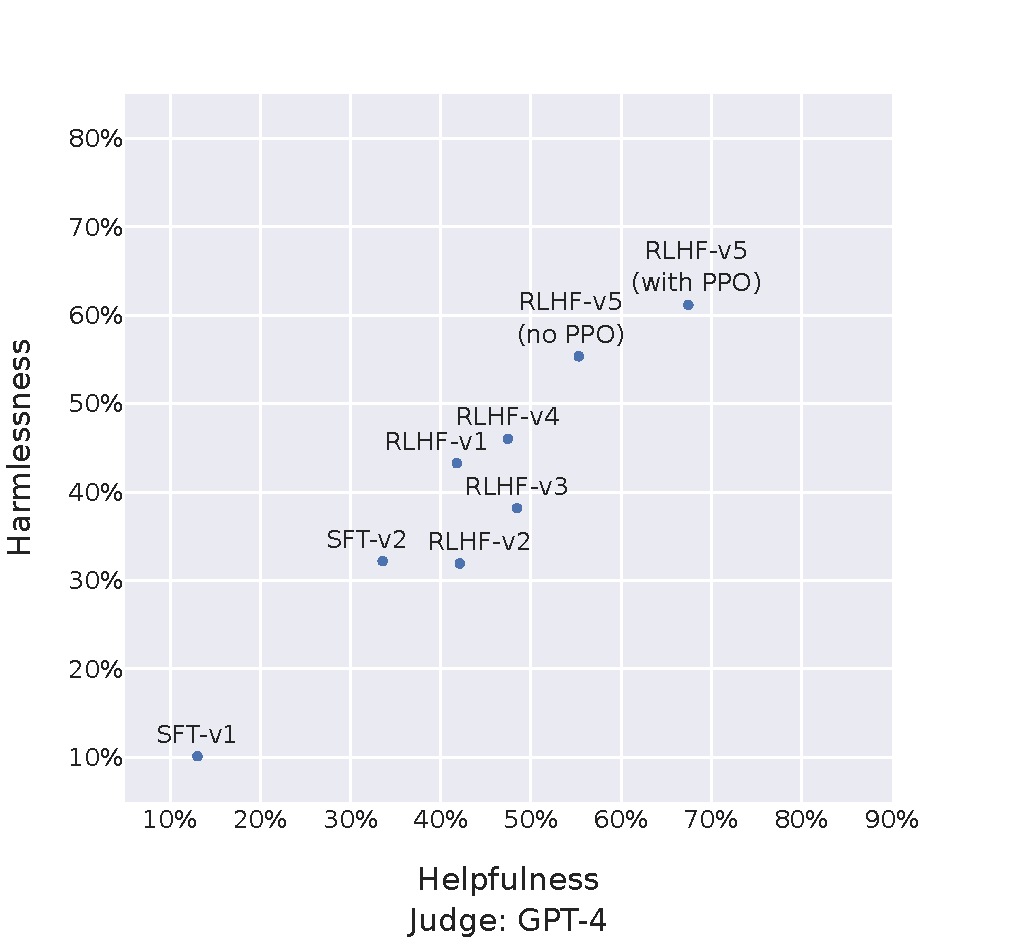
\includegraphics[width=0.7\textwidth]{evolution_of_chatllama_GPT4.pdf}
    \caption{Порівняння ефективності роботи моделі LLaMA 2 Chat проти ChatGPT на різних ітераціях RLHF -- в якості оцінювача виступає модель GPT-4 \cite{touvron2023llama2openfoundation}.}
    \label{fig:llama2_performance}
\end{figure}

\paragraph{Альтернативи RLHF}

Окрім RLHF існують альтернативні методи до тонкого налаштування ВММ, які спрямовані на спрощення процесу та зменшення залежності від людського зворотного зв'язку. У цьому підрозділі буде розглянуто декілька альтернативних методів.

\begin{itemize}
    \item {Пряме оптимізування зворотного зв'язку (Direct Preference Optimization, DPO)} \cite{rafailov2024directpreferenceoptimizationlanguage}: Метод DPO пропонує оптимізувати модель безпосередньо на основі людського зворотного зв'язку без необхідності у навчанні окремої моделі винагород та використання методу навчання з підкріпленням. Замість цього використовується керована функція втрат для тонкого налаштування моделі. Дана функція враховує уподобання між парами відповідей, що дозволяє цілеспрямовано налаштовувати модель на основі людського зворотного зв'язку, таким чином спрощуючи процес навчання.

    \item {Навчання з підкріпленням із зворотним зв'язком від ШІ (Reinforcement Learning with AI Feedback, RLAIF)} \cite{lee2024rlaifvsrlhfscaling}: Метод RLAIF замінює людський зворотний зв'язок на зворотний зв'язок від великої мовної моделі при навчанні моделі винагород. Це зменшує залежність від необхідності підготовки анотацій людини та показує не схожі результати роботи у порівнянні із традиційними методами з використанням RLHF. RLAIF використовує потужну ВММ для генерації оцінок та коментарів до відповідей моделі, що дозволяє автоматизувати процес навчання на основі зворотного зв'язку.

    \item {Навчання людського зворотного зв'язку за допомогою контрастивного навчання (Contrastive Preference Learning, CPL)} \cite{hejna2024contrastivepreferencelearninglearning}: Метод CPL використовує контрастивну функцію втрат для навчання моделі на основі порівнянь пар відповідей. Це спрощує процес тонкого налаштування без використання RL. Перевагою CPL є ефективне використання даних з парним ранжуванням відповідей, що сприяє кращому навчанню моделі на основі людського зворотного зв'язку.

    \item {Розширене самостійне навчання з підкріпленням (Reinforced Self-Training, ReST)} \cite{gulcehre2023reinforcedselftrainingrestlanguage}: Метод ReST поєднує самостійне навчання з підкріпленням, використовуючи ітеративний підхід до відбору та тренування на найбільш якісних прикладах, що поліпшує ефективність у  порівнянні зі стандартними методами RLHF. ReST генерує нові дані для тренування, вибираючи відповіді з високою винагородою та використовує їх для подальшого тонкого налаштування моделі. Це зменшує залежність від людського зворотного зв'язку та покращує загальну ефективність навчання.
    
    \item {Hindsight Instruction Relabeling (HIR)} \cite{zhang2023wisdomhindsightmakeslanguage}: Метод HIR передбачає повторне маркування інструкцій на основі відповідей, згенерованих моделлю. Це дозволяє використовувати неточні відповіді, що були раніше згенеровані моделлю, як корисні навчальні дані для керованого навчання. Якщо модель дає відповідь, яка не відповідає початковій інструкції, HIR змінює інструкцію таким чином, щоб вона відповідала згенерованій відповіді. Після чого отримана пара використовується для подальшого тренування моделі.

    \item {Constitutional AI} \cite{bai2022constitutionalaiharmlessnessai}: У методі Constitutional AI пропонується самостійне навчання моделі на основі набору правил наданих людьми. Модель генерує та автоматично відбирає відповіді без прямого людського зворотного зв'язку, використовуючи ці правила для оцінки та вдосконалення своїх відповідей. Цей підхід дозволяє зменшити обсяг процесу анотації людьми, що необхідна для тренування моделі, та забезпечує більш контрольовані результати згенерованих відповідей.
\end{itemize}

\subsection{Генерація з доповненням через пошук}
Генерація з доповненням через пошук (Retrieval-Augmented Generation, RAG) -- це підхід у машинному навчанні, що поєднує методи підготовки та запитування даних для покращення якості згенерованого тексту. Він складається з двох основних компонентів:
\begin{enumerate}
    \item {Підготовка даних (Ingestion):} До того як модель використовується у роботі, спочатку відбувається підготовка бази знань. В якості бази знань може використовуватися великий текстовий корпус, такий як, наприклад, Вікіпедія. Дані проходять попередні етапи обробки та зберігаються зазвичай у векторному представленні задля зручного пошуку на наступних етапах RAG.
    \item {Запитування (Querying):} Після отримання запиту модель шукає релевантну інформацію у базі даних та використовує задля підготовки відповіді.
\end{enumerate}

У напрямку роботи з математичними задачами та великими мовними моделями підхід RAG може бути корисним у таких аспектах, як розв'язання математичних задач та підвищення точності роботи мовних моделей за рахунок використання теоретичної бази знань:
\begin{itemize}
    \item Замість того, щоб покладатися лише на знання моделі, RAG може отримувати схожі задачі з наявного набору даних (наприклад, наборів математичних задач) і використовувати їх як приклади для розв’язання.
    \item Модель може обґрунтовувати логіку побудови розв'язання та задіювати відповідні математичні концепції.
    \item Великі мовні моделі часто мають складнощі з точністю при роботі з числовими перетвореннями. Використання RAG дозволяє отримувати перевірені розв’язки або теоретичні пояснення задля поліпшення роботи з числовими даними.
    \item Метод може допомогти у розв’язанні складних задач, розбиваючи їх на більш прості підзадачі за допомогою знайдених аналогів.
\end{itemize}

Одним з прикладів використання даного методу у освітніх цілях є автоматизація підготовки та перевірки інтерактивних запитань і відповідей при навчанні шкільної математики. Без додаткових методів мовні моделі можуть генерувати помилкові або невідповідні відповіді, які не узгоджуються з навчальною програмою. Один із методів до підвищення якості відповідей -- використання RAG, де модель використовує перевірені джерела знань для покращення своїх відповідей. Дослідження показують, що включення матеріалів із відкритих навчальних ресурсів у запити до ВММ може покращити якість відповідей на математичні питання, проте існує компроміс між відповідністю підручникам і якістю сприйняття наданих відповідей учнями \cite{levonian2023retrievalaugmentedgenerationimprovemath}.

\paragraph{Підготовка даних}

\begin{figure}[h]
    \centering
    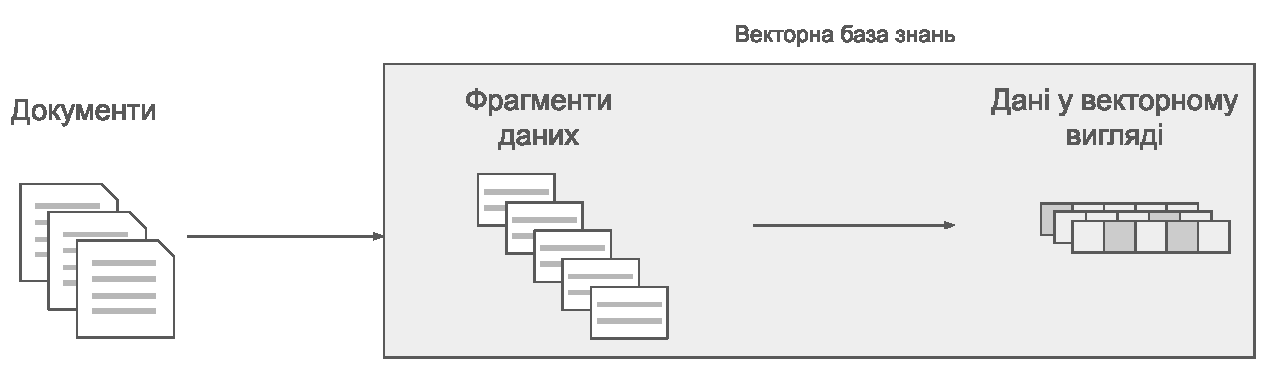
\includegraphics[width=1\textwidth]{rag_ingestion.pdf}
    \caption{Попередній етап RAG -- підготовка даних для збереження у векторній базі знань.}
    \label{fig:rag_ingestion}
\end{figure}

Як видно з рис.~\ref{fig:rag_ingestion}, процес отримання даних розбивається на кілька етапів, які виконуються наступним чином:

\begin{enumerate}
    \item {Завантаження даних у текстовий формат}: На першому кроці дані отримуються у звичайному текстовому вигляді (наприклад, набір документів), які зберігаються разом.
    \item {Розбиття тексту на фрагменти}: Оскільки мовні моделі мають обмеження на довжину контекстного вінка, відбувається фрагментація збереженої інформації.
    \item {Вбудовування тексту}: Після цього дані переводять у векторне представлення для кожного фрагмента тексту, що дозволяє виконувати пошук релевантних елементів інформації на подальших кроках.
    \item {Завантаження векторних представлень у базу знань}: Отримані вектори та текстові фрагменти зберігаються у спеціалізоване сховище -- векторна база знань, що забезпечує швидкий пошук релевантної інформації. Додаткове збереження фрагментів у текстовому вигляді необхідне задля повернення відповідної інформації у звичайному для людини вигляді (тобто тексту).
\end{enumerate}

\paragraph{Запитування даних}

\begin{figure}[h]
    \centering
    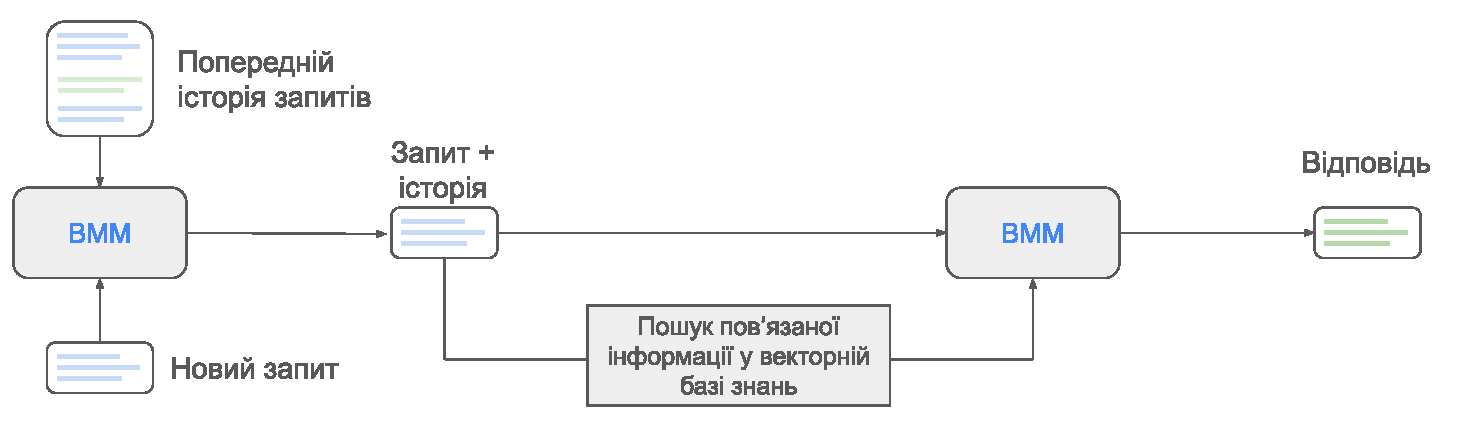
\includegraphics[width=1\textwidth]{rag_querying.pdf}
    \caption{Етап RAG -- пошук релевантної інформації у векторній базі знань.}
    \label{fig:rag_querying}
\end{figure}

Процес запитування даних також можна розбити на кілька етапів, як показано на рис.~\ref{fig:rag_querying}, які здебільшого базуються на використанні вхідних запитів:

\begin{enumerate}
    \item {Об'єднання історії запитів та нового запиту}: Формування єдиного запиту задля врахування контексту попередньої частини діалогу.
    \item {Пошук релевантної інформації}: За допомогою підготовленої бази знань, знаходяться релевантні фрагменти інформації.
    \item {Генерація відповіді}: На основі сформованого запиту та знайденої релевантної інформації модель повертає відповідь.
\end{enumerate}

\subsection{Прихований процес міркування в мовних моделях}

З появою великих нейронних мереж та зростанням їх можливостей обробляти текстові дані, стало актуальним формування внутрішнього процесу операцій міркування моделей під час генерації відповідей. Особливу увагу слід приділити новим методам, які змінюють парадигму генерації висновків.

Ідея використання ВММ зосереджених на міркуванні не є зовсім новою. Попередні дослідження, зокрема модель Self-Taught Reasoner (STaR) ~\cite{zelikman2022starbootstrappingreasoningreasoning}, вже розглядали концепцію тренування моделей виводити обґрунтування з кількох прикладів. Метод STaR дозволяє моделям покращувати свою ефективність при генерації відповідей.

\begin{enumerate}
    \item {Внутрішнє обмірковування}: При отриманні запиту модель спочатку веде внутрішній монолог. На цьому етапі вона генерує кілька можливих відповідей і оцінює їх за наперед визначеними критеріями. Цей процес нагадує мозковий штурм і фільтрацію ідей перед вибором найкращого варіанту.
    \item {Генерація відповіді}: Після внутрішнього обмірковування модель обирає найбільш раціональну та зв’язну відповідь для користувача. За рахунок цього, фінальний результат буде точнішим і краще відповідає завданню у порівнянні з традиційними методами генерації відповідей за допомогою ВММ.
\end{enumerate}

\paragraph{Метод Quiet-STaR}
Як згадувалося у попередніх підрозділах, для структуризації внутрішнього процесу операцій міркування широко застосовується техніка ланцюжка думок, яка дозволяє моделі послідовно розбивати вхідний запит на набір кроків. Однак, сучасні методи спрямовані не лише на розбиття запиту, а й на тренування моделі самостійно поліпшувати власні міркування перед тим, як запропонувати фінальну відповідь. До таких можна віднести метод Quiet-STaR (Sequential Thought and Rationale), який було описано у роботі \cite{zelikman2024quietstarlanguagemodelsteach}. Основна ідея цього методу полягає у послідовному виконанні наступних етапів:
\begin{enumerate}
    \item {Міркування:} Для кожного вхідного токена модель генерує кілька варіантів ланцюжка думок у паралельному режимі, створюючи кілька варіацій міркування.
    \item {Обговорення:} Отримані результати міркування поєднуються, кінцевий результат формується на основі співвідношення впливу згенерованих токенів міркувань та початкового запиту.
    \item {Навчання:} Під час наступного тренування модель оптимізує свої параметри, винагороджуючи ті ланцюжки міркувань, які призводять до коректних прогнозів, та караючи невдалий алгоритм розумування.
\end{enumerate}

Роботу методу можна бачити на рис.~\ref{fig:quiet_star_scheme}.

\begin{figure}[h]
    \centering
    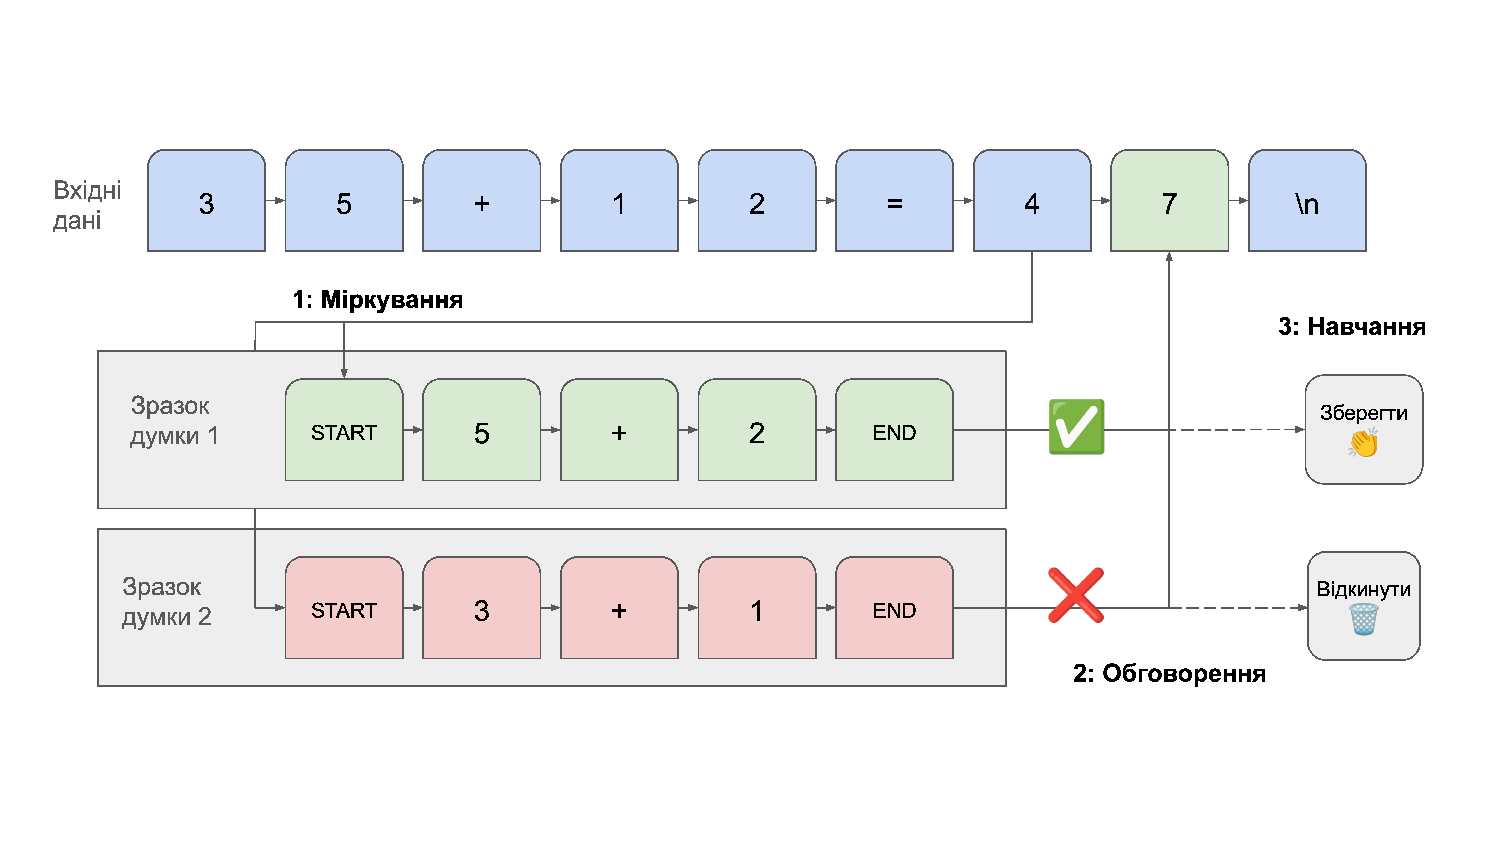
\includegraphics[width=1\textwidth]{quiet_star_scheme.pdf}
    \caption{Схематичне представлення методу Quiet-STaR: послідовне виконання етапів міркування, обговорення та навчання.}
    \label{fig:quiet_star_scheme}
\end{figure}

На кожному етапі міркування відбувається за допомогою великої мовної моделі. Основними перевагами даного методу є:

\begin{itemize}
    \item {Підвищена точність у складних завданнях}: Завдяки внутрішньому міркуванню Quiet-STaR ефективніше справляється зі складними завданнями. Це особливо корисно для задач, що вимагають логічного висновку, розв’язання проблем та багатокрокового міркування. Внутрішній монолог допомагає розбивати проблему на підзадачі та підходити до її вирішення методично, що призводить до точніших результатів.

    \item {Зменшення потреби у додаткову навчанні}: Традиційні ВММ часто потребують значних ресурсів під час тонкого налаштування на специфічних наборах даних для якісного виконання спеціалізованих завдань. Quiet-STaR знижує цю потребу, використовуючи внутрішнє міркування, що дозволяє моделі краще узагальнювати знання та ефективно працювати з різними завданнями без додаткового навчання.

    \item {Покращена інтерпретованість}: Однією з проблем ВММ є непрозорість процесу прийняття рішень. Quiet-STaR вирішує цю проблему, надаючи обґрунтування своїх відповідей. Внутрішній монолог можна зробити видимим, що дає змогу аналізувати процес міркувань моделі. Це підвищує зрозумілість та довіру до її відповідей.
\end{itemize}

Впровадження Quiet-STaR дозволяє моделі не лише прогнозувати наступний токен, але й формувати власну логічну аргументацію, що значно покращує точність відповідей на складні питання, а також підвищує здатність моделі до вирішення завдань, що вимагають математичних обчислень або логічного мислення. Результати тестування даних моделей демонструють, що чим довший внутрішній процес міркування, тим більш якісні висновки, до яких приходить модель.

Одним з прикладів використання запропонованого методу є модель o1 від OpenAI\footnote{\url{https://platform.openai.com/docs/guides/reasoning}.}, які започаткували серію моделей міркування (Reasoning models). Для таких моделей, як наприклад o1, окрім стандартної генерації відповіді, додається окремий етап, який виглядає як внутрішній процес міркування. Завдяки цьому модель проводить додатковий аналіз, перевіряє та покращує свої розрахунки, що дозволяє досягти більш високої точності, зокрема у більш складних математичних завданнях.

Моделі o1 вводять токени розуміння (reasoning tokens). Моделі використовують ці токени розуміння для ``міркування'', розбиваючи своє розуміння запиту на кроки, після чого розглядаючи кілька варіантів потенційно згенерованої відповіді. Після генерації токенів розуміння модель будує фінальну відповідь, а токени розуміння видаляються з її контекстного вікна як можна бачити на рис.~\ref{fig:reasoning_window}.

\begin{figure}[!h]
    \centering
    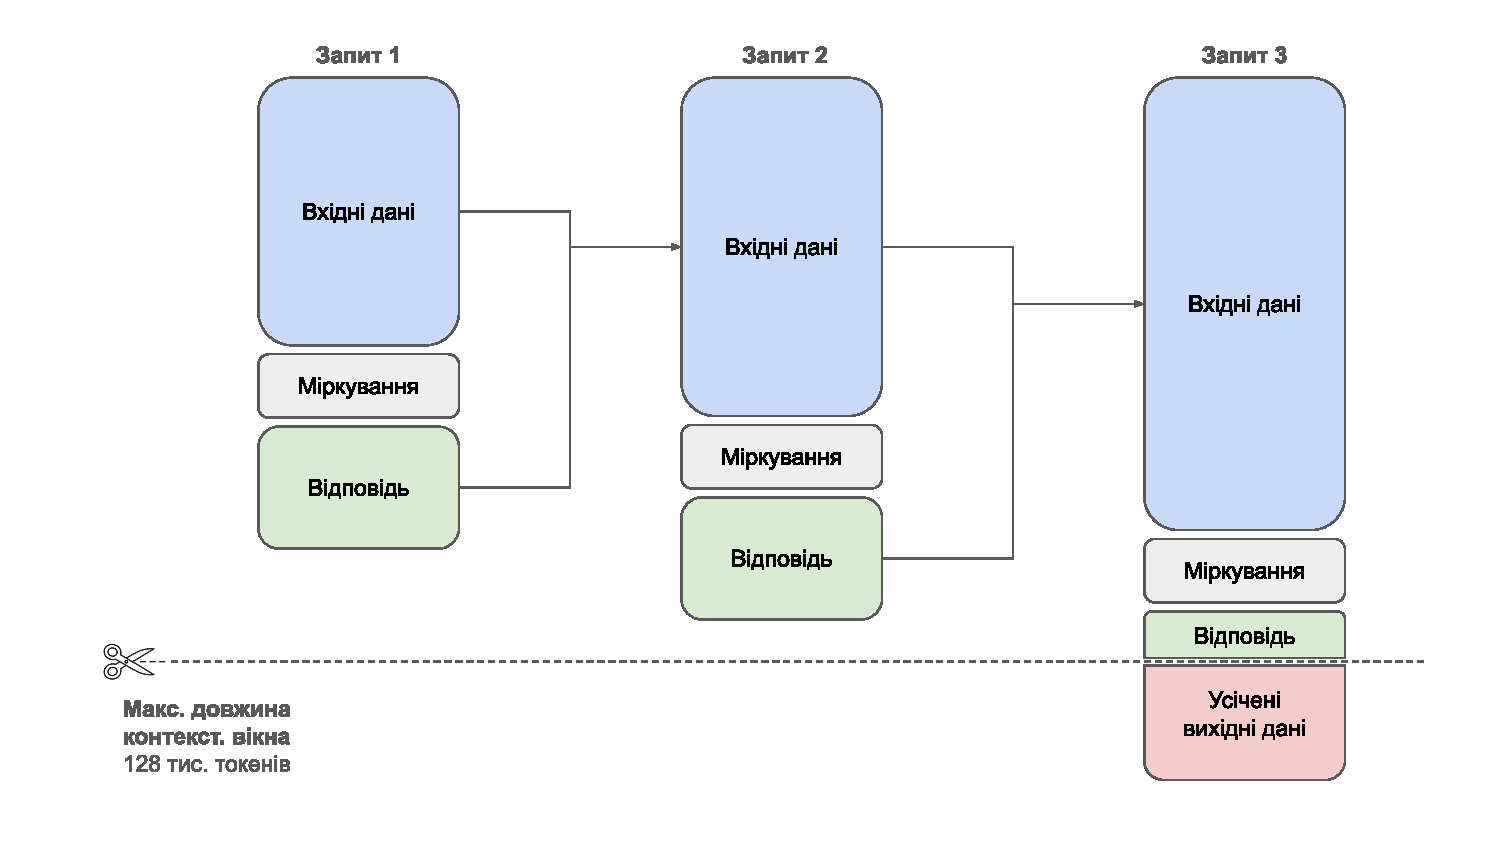
\includegraphics[width=0.9\textwidth]{reasoning_tokens.pdf}
    \caption{Приклад діалогу між користувачем та моделлю. Вхідні та вихідні токени з кожного кроку зберігаються у кеш, тоді як токени розуміння видаляються.}
    \label{fig:reasoning_window}
\end{figure}

При роботі з моделями міркуванням, користувач може спостерігати появу окремої частини відповіді -- думок, що демонструє внутрішній процес міркування моделі, як це, наприклад, показано на рис.~\ref{fig:reasoning_example}.

% https://chatgpt.com/c/67adb076-608c-8008-b06f-34af5da33bbc
\begin{figure}[!h]
    \centering
    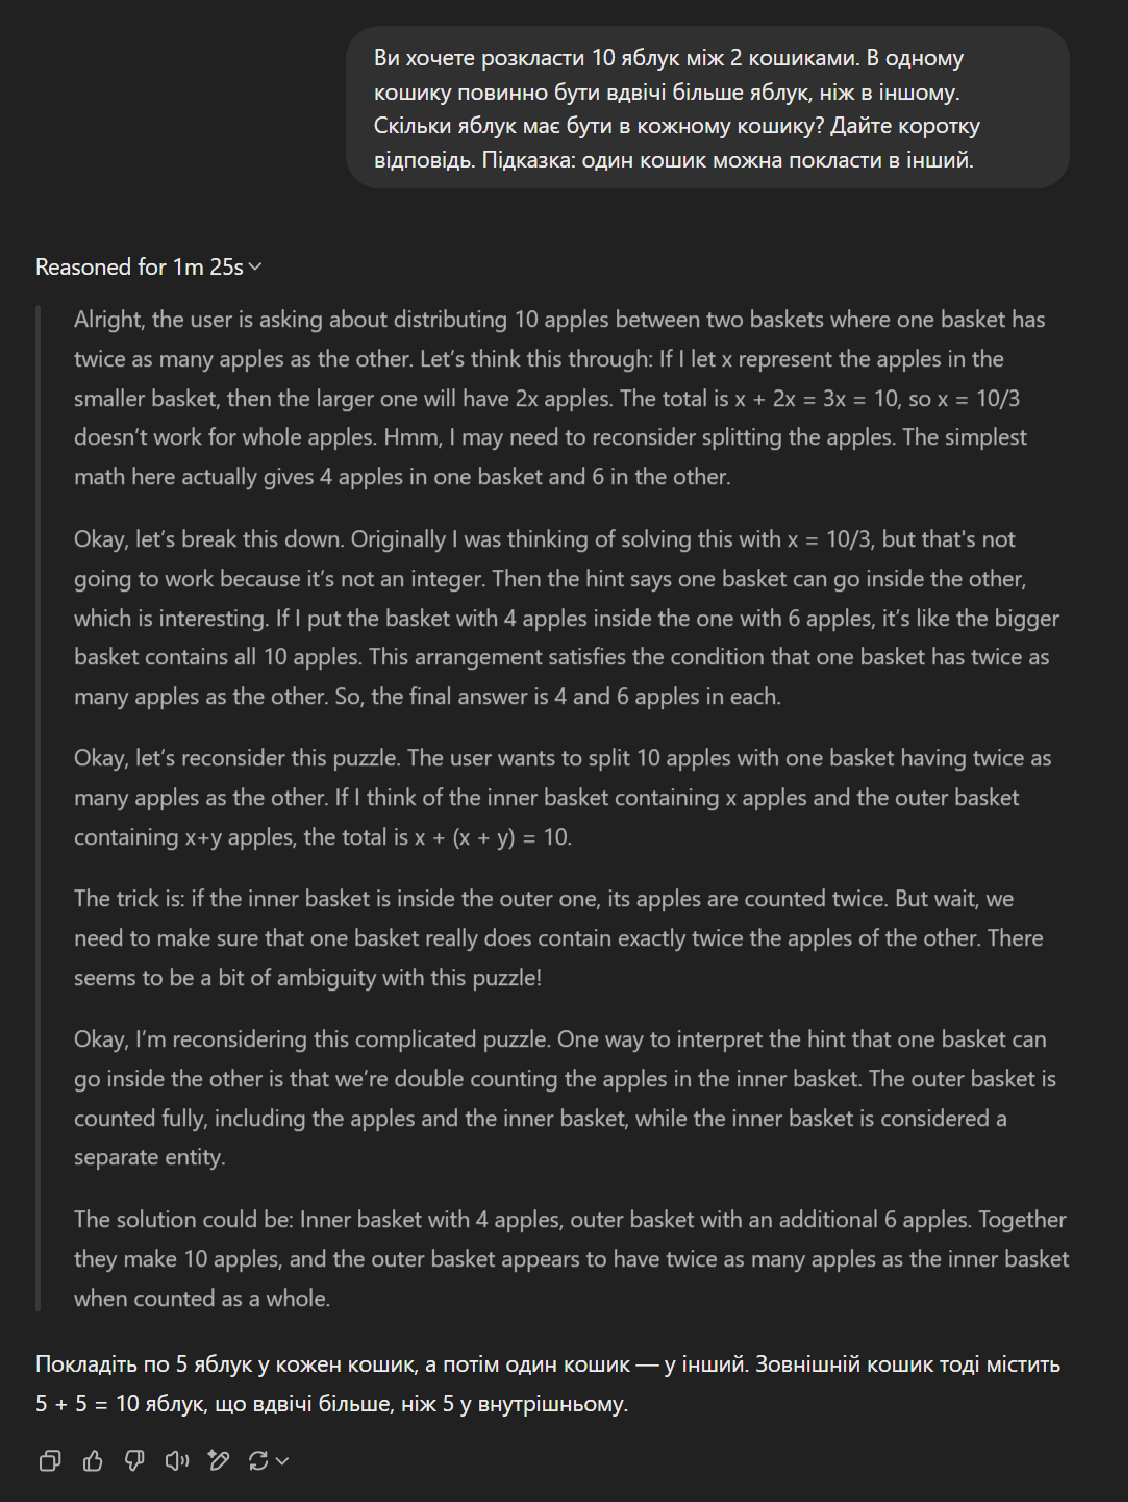
\includegraphics[width=0.9\textwidth]{reasoning_example.pdf}
    \caption{Приклад розв'язання задачі з моделлю, що демонструє процес ``міркування''. Не зважаючи на те, що запит було задано українською, внутрішнє міркування моделі відбувається англійською.}
    \label{fig:reasoning_example}
\end{figure}

Таким чином, перехід від традиційних мовних моделей до моделей міркування свідчить про нову парадигму під час генерації розв'язків, де важливим стає не лише збереження отриманих знань під час тренування, але й розвитку динамічних стратегій розуміння та планування. Це відкриває шлях до створення \emph{центрів міркування (core of reasoning)} -- окремих модулів, спеціалізованих на динамічному міркуванні та пошуку оптимальних рішень, що забезпечує не тільки збільшення автономності моделей, а й їх адаптивності для різних агентних застосувань, а також систем з використанням RAG.

У підсумку, комбінована інтеграція методів CoT та Quiet-STaR дає змогу моделі навчатися міркувати, використовувати власні внутрішні міркування для оптимізації генерації відповідей і досягати більшої точності при вирішенні складних завдань, що є важливим кроком у розвитку сучасних систем штучного інтелекту. На даний момент цей підхід є одним з передових задля досягнення найкращої точності при розв'язанні математичних задач при взаємодії з великими мовними моделями.

% https://www.deeplearning.ai/the-batch/issue-286/
\paragraph{Використання навчання з підкріпленням для генерації ланцюга міркувань.}

Нещодавні моделі, такі як DeepSeek-R1 \cite{deepseekai2025deepseekr1incentivizingreasoningcapability} та Kimi k1.5 \cite{kimiteam2025kimik15scalingreinforcement} показали, що RL можна ефективно використовувати для поліпшення ланцюжка міркувань у ВММ особливо у задачах, які потребуються точності та логіки при формуванні міркувань. Навчання з підкріпленням винагороджує модель за правильне розв'язання задач, стимулюючи її генерувати послідовності висновків, які ведуть до правильного результату.

Особливості підходу:

\begin{itemize}
    \item {Генерація ланцюжка міркувань}: Моделі навчаються генерувати детальні послідовності міркувань для вирішення складних задач.
    \item {Самостійне виявлення стратегій}: Після попереднього навчання з підкріпленням моделі здатні самостійно розробляти стратегії розв'язання задач.
    \item {Оптимізація довжини відповідей}: Додаткове навчання з підкріпленням використовується для скорочення надмірно довгих відповідей без втрати точності.
\end{itemize}

% https://garymarcus.substack.com/p/alphaproof-alphageometry-chatgpt
\section{Інтегроване розуміння з інструментами}

Хоча запропоновані у останніх роках методи задля покращення точності роботи ВММ призвели до кращих результатів на відповідних наборах даних, питання їхньої точності у загальній здатності до міркування все ще залишається відкритим. У той час як моделі здатні достатньо вдало виконувати задачі перекладу текстів між мовами, вони не показують необхідної точності при роботі з логікою та міркуванням \cite{bubeck2023sparksartificialgeneralintelligence}.

Відповідно, одним з перспективним досліджень є автоматизація розв'язання математичних задач та формалізації математичних текстів за допомогою великих мовних моделей. Одним з методів, яких можна віднести до даного підходу є ToRA -- Інтегроване розуміння з інструментами (Tool-integrated Reasoning Agents).

\subsection{Використання ВММ та інструментів символьних обчислень}
Інтегроване розуміння з інструментами для математичних обчислень дозволяє покращити точність розв'язань та забезпечити перевірку результатів за рахунок проміжних (зазвичай прихованих) обчислень. Вперше ідея була запропонована у роботі \cite{gao2023palprogramaidedlanguagemodels}, які запропонували Program-Aided Language models (PAL) метод, який використовує ВММ для читання задач природною мовою разом з використанням додаткових програм задля проміжних кроків розумного мислення, після чого передає згенерований код на виконання до середовища виконання, такого як інтерпретатор Python. Завдяки PAL, інтерпретація запиту з природної мови у набір інструкцій залишається єдиним завданням навчання для ВММ, тоді як безпосереднє виконання роботи передається інтерпретатору. Ця взаємодія між нейронною ВММ та символічним інтерпретатором була протестована на 13 математичних, символьних та алгоритмічних метриках, у тому числі на BIG-Bench Hard. Результати показали, що у завданнях на логічне мислення на природній мові, генерація коду за допомогою ВММ та розуміння через інтерпретатор Python призводить до більш точних результатів, ніж значно більші моделі. Наприклад, PAL з використанням Codex досягає передових показників few-shot на тестовому наборі GSM8K математичних словесних задач, перевищуючи ВММ PaLM-540B, який використовує ланцюг міркувань, на 15\% більш точним при роботі. Ідея пояснена на рис.~\ref{fig:pal-overview}.

\begin{figure}[!h]
    \centering
    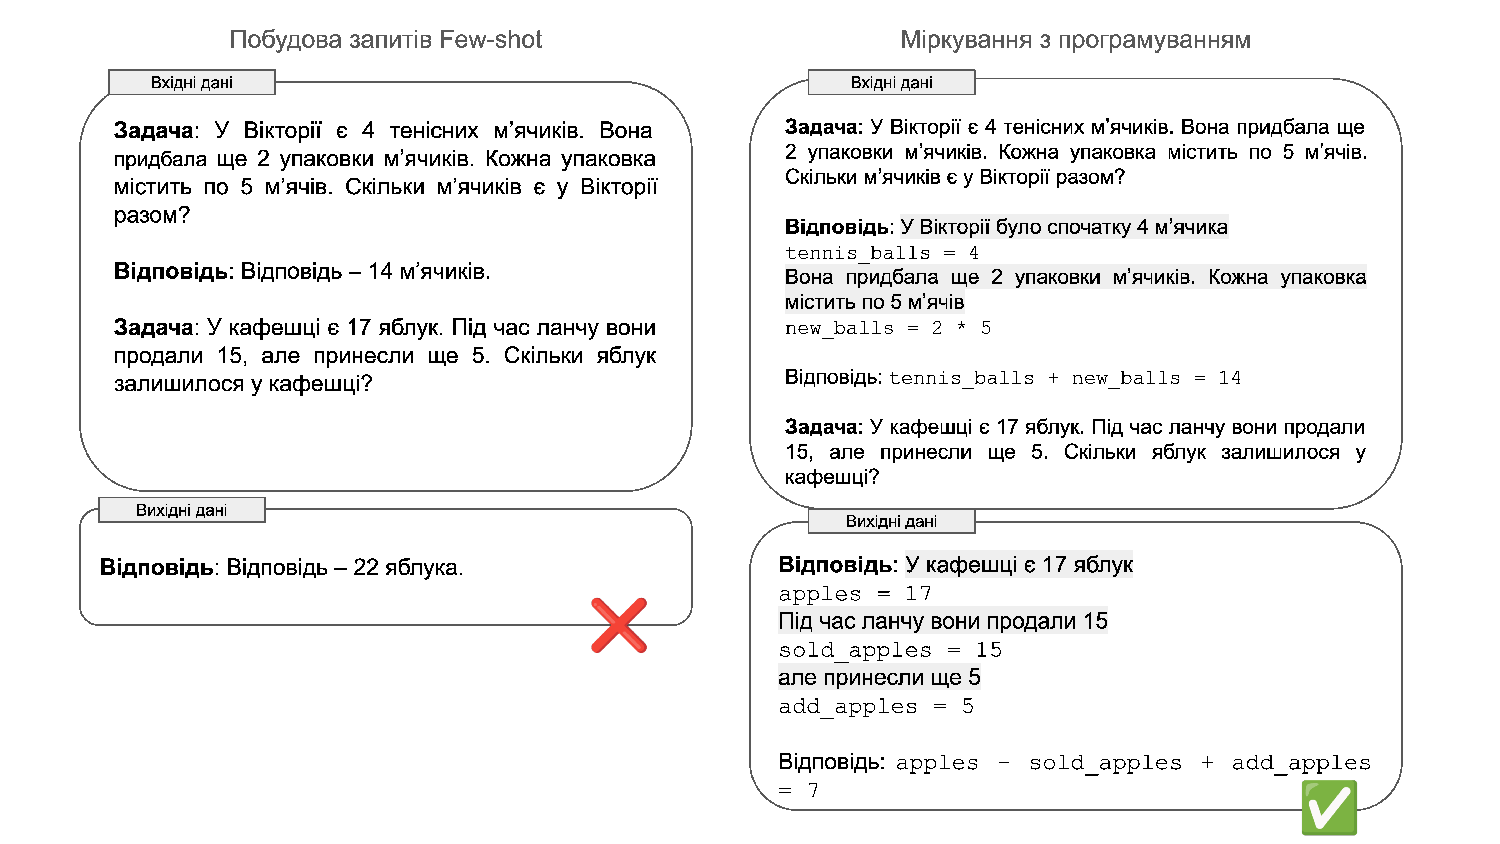
\includegraphics[width=1\textwidth]{pal_overview.pdf}
    \caption{PAL генерує програму на Python для вирішення завдання з його опису на природній мові.}
    \label{fig:pal-overview}
\end{figure}

У роботі \cite{gou2024toratoolintegratedreasoningagent} було запропоновано метод ToRA. ToRA -- це серія агентів для інтегрованого розумового мислення, розроблених для вирішення складних математичних задач шляхом взаємодії з інструментами для проведення символьних обчислень. ToRA приховано інтегрує розуміння природної мови з використанням зовнішніх інструментів, тим самим об'єднуючи аналітичні здібності мови та обчислювальну ефективність додаткових інструментів. Для навчання ToRA формується інтерактивні траєкторії використання інструментів на математичних наборах даних, застосовуємо навчання наслідування на анотаціях та пропонуємо формування простору вихідних даних для подальшого вдосконалення поведінки розумного мислення моделей. В результаті моделі ToRA значно перевершують відкриті моделі на 10 математичних наборах завдань на логічне мислення у всіх конфігураціях з абсолютними покращеннями від 13\% до 19\% в середньому. Особливо варто відзначити, що ToRA-7B досягає 44,6\% на конкурсі рівня MATH, перевищуючи найкращу відкриту модель WizardMath-70B на 22\% в абсолютних показниках. ToRA-Code-34B також є першою відкритою моделлю, яка досягає точності понад 50\% на MATH, що значно перевищує результати GPT-4 з chain-of-thought, та є конкурентоспроможною з GPT-4 у вирішенні завдань з програмами. Додатково, автори провели вичерпний аналіз переваг та залишкових викликів взаємодії з інструментами для математичного мислення, надаючи цінні інсайти для майбутніх досліджень. Ідея пояснена на рис.~\ref{fig:tora-example}.

\begin{figure}[!h]
    \centering
    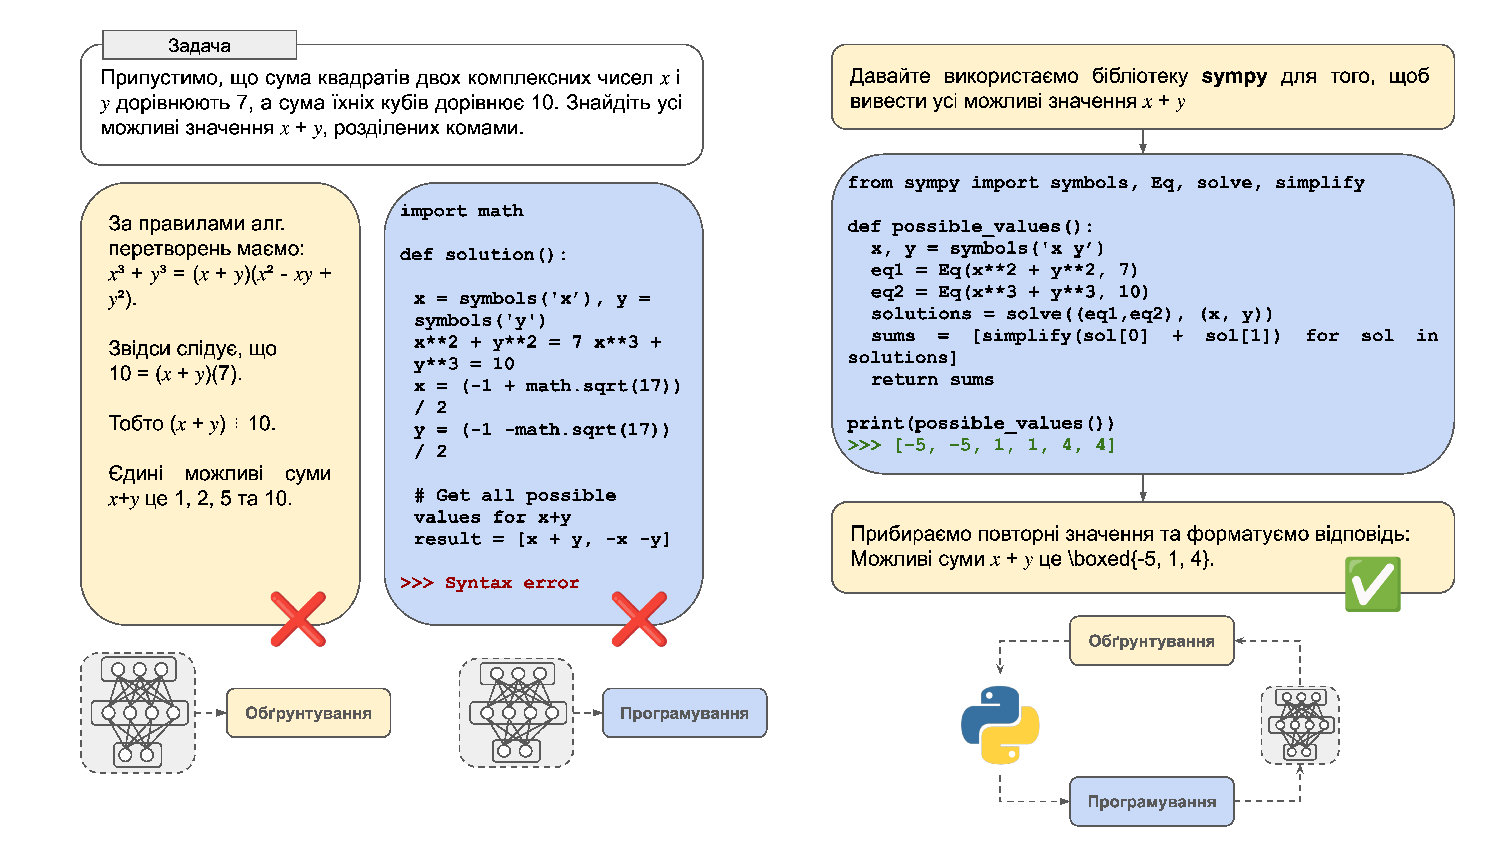
\includegraphics[width=1\textwidth]{tora_example.pdf}
    \caption{Основний приклад взаємодії з інструментом, яка чергує обґрунтування з використанням програмних інструментів.}
    \label{fig:tora-example}
\end{figure}

Даний підхід є ефективним до розв'язання алгебраїчних задач та роботи з даними, де точність обрахунків є важливою.

\subsection{Використання ВММ для систем автоматизації доведень}

Для автоматизації математичного міркування було запропоновано підхід \cite{nikolaiev2024neuralform}, що інтегрує великі мовні моделі із системами автоматичного доведення. Цей метод передбачає отримання умови задачі у вигляді природної мови, перекладом до формалізованого вигляду за допомогою ВММ, подальшу перевірку та генерацію розв’язку у формальному вигляді з використанням системи автоматизації доведень, а потім переведення отриманого розв'язання до початкового формату задля зручного сприйняття користувачем. Рис.~\ref{fig:formalisation_with_llms} ілюструє основні етапи даної процедури.

\begin{figure}[!h]
    \centering
    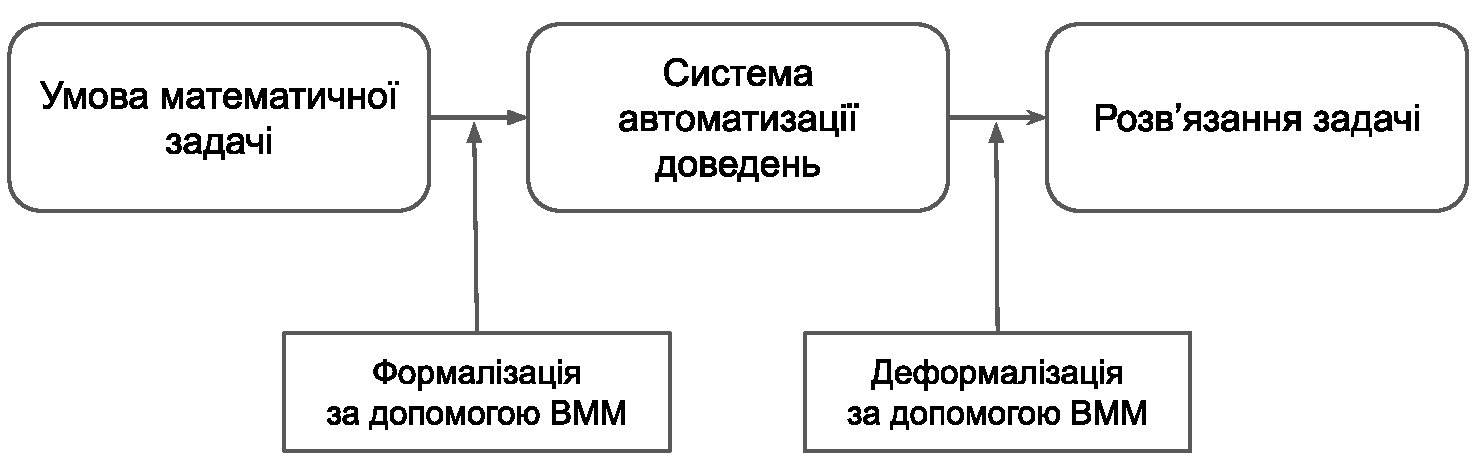
\includegraphics[width=1\textwidth]{formalisation_with_llms.pdf}
    \caption{Опис процедури для формалізації та деформалізації заданої умови та розв’язання задачі.}
    \label{fig:formalisation_with_llms}
\end{figure}

Нижче приклад використання методу у 5 кроків:

\begin{itemize}
    \item \textbf{Крок 1.} Початкова задача задана на вхід англійською мовою:
\begin{lstlisting}[language=json, breaklines=true]
Prove that for any natural number n, the sum of the first n odd natural numbers is n^2.
\end{lstlisting}
    
    \item \textbf{Крок 2.} Звернення до ВММ для переведення умови у формальний вигляд:
\begin{lstlisting}[language=json, breaklines=true]
{"content": "Translate the following mathematical statement                         into LEAN: {Problem statement in natural language text}."}
\end{lstlisting}
    
    \item \textbf{Крок 3.} Формалізація умови та розв’язання задачі за допомогою системи LEAN:
    \newpage
    
\begin{lstlisting}[language=json, breaklines=true]
{
import data.nat.parity
open nat
-- The statement of the theorem
theorem sum_of_first_n_odd_numbers (n : nat) : sum i in range n, (2 * i + 1) = n^2 :=
begin
  -- We will prove this by induction on n
  induction n with n ih,
  -- Base case: n = 1
  { 
    -- The sum from 1 to 1 is 1, and 1^2 is also 1
    simp, 
  },
  -- Inductive step: assume it is true for n, prove for n+1
  { 
    -- We need to show sum i in range (n + 1), (2 * i + 1) = (n + 1)^2
    -- The sum can be broken down into the sum for range n plus the last term (2 * n + 1)
    rw sum_range_succ,
    -- Using the induction hypothesis ih: sum i in range n, (2 * i + 1) = n^2
    rw ih,
    -- Thus, n^2 + (2 * n + 1) = (n + 1)^2
    -- Simplifying the right hand side: expand (n + 1)^2 to n^2 + 2 * n + 1
    simp,
  }
end
}
\end{lstlisting}
    
    \item \textbf{Крок 4.} Проміжний крок – звернення до GPT-4o:
\begin{lstlisting}[language=json, breaklines=true]
{"content": "Translate the following mathematical text into natural                 language: {Problem statement in LEAN}."}
\end{lstlisting}
    
    \item \textbf{Крок 5.} Після цього формалізований варіант задачі переговорюється до наступного викладу як зазначено у таблиці~\ref{tab:nl_solution}.

    \begin{figure}[h!]
        \centering
        \small
        \captionof{table}{Solution in natural language representation.}
        \label{tab:nl_solution}
        \begin{tabular}{|p{0.80\linewidth}|}
        \hline
        \textbf{Розв'язання задачі про суму непарних чисел.} \\
            \hline
            To prove that the sum of the first n odd natural numbers is $n^{2}$, we use mathematical induction: \\
            1) Base case: For $n = 1$, the sum is 1, which equals $1^{2}$. \\[5pt]
            2) Inductive step: Assume the sum of the first n odd natural numbers is $n^{2}$. We need to prove it for $n + 1$. \\
            \quad The $(n+1)$-th odd number is $2n + 1$. Thus, the sum of the first n + 1 odd numbers is \\
            \quad $(1 + 3 + 5 + … + (2n - 1)) + (2n + 1)$. \\
            \quad By the inductive hypothesis, this equals $n^{2} + (2n + 1) = n^{2} + 2n + 1 = (n + 1)^{2}$. \\
            Thus, by induction, for any natural number n, the sum of the first n odd natural numbers is $n^{2}$. \\
            \hline
        \end{tabular}
    \end{figure}

\end{itemize}

\paragraph{Можливості методу на рівні IMO}
Гарним прикладом у роботі з математичними задачами високої складності є нещодавня система AlphaProof, розроблена Google DeepMind -- нейро-символьна система, що складається з нейронної мовної моделі та символьного двигуна дедукції, які разом працюють для знаходження доказів складних геометричних теорем. Система запропонувала ефективний спосіб автоматичної формалізації даних за допомогою ВММ Gemini для створення повної бібліотеки формальних задач різної складності. Цей підхід долає розрив між розумінням природної мови та формальним розв'язанням задач, підвищуючи точність і надійність математичних міркувань та розв'язання задач рівня Міжнародної математичної олімпіади (International Mathematical Olympiad, IMO) з використанням символьних методів. У поєднанні з оновленою варіацією раніше опублікованої AlphaGeometry \cite{Trinh2024SolvingOG}, система змогла розв'язати 4 з 6 математичних задач з останнього змагання IMO-2024\footnote{\url{https://dpmd.ai/imo-silver}.}. Проте, на відміну від інших математичних задач, комбінаторні задачі залишаються нерозв'язаними, підкреслюючи комбінаторику як перспективну область для майбутніх досліджень. Це, ймовірно, обумовлено властивістю комбінаторних задач, які вимагають від систем високої точності в опрацюванні семантики та використанні відповідних методів і теорем для знаходження правильних розв'язків.

%%%%%%%%%%%%%%%%%%%%%%%%%%%%%%%%%%%%%%
\section{Недоліки та переваги існуючих методів}

Як вже було зазначено раніше традиційні мовні моделі навчаються прогнозувати наступне слово у реченні за допомогою великих наборів даних і механізмів, таких як механізм само-уваги. Процес навчання у даних моделях складається з двох основних етапів: (i) попереднє тренування, на якому модель здобуває загальне розуміння мови; та (ii) доопрацювання, де модель адаптується до конкретних завдань і вирівнюється з людським зворотнім зв'язком.

Як згадувалося раніше деякі провідні моделі, зокрема ті, що використовують архітектуру MoE, оптимізують обчислювальні ресурси завдяки динамічному механізму маршрутизації, який вибирає відповідних ``експертів'' для обробки конкретного запиту.

Великі мовні моделі досягли значного прогресу в різних мовних завданнях, проте вони все ще стикаються з труднощами при розв'язанні задач складної математики. Зокрема мовні моделі продемонстрували здатність розв'язувати арифметичні задачі, проводити символьні обчислення та виконувати логічне мислення, коли їм надається кілька прикладів під час тестування (Zero-shot, Few-shot). Але найбільшого прогресу досягли моделі з інтегрованими методами ланцюжка думок (chain-of-thought), які використовують ВММ для розуміння опису задачі шляхом розкладання її на кроки та послідовного виконання кожного відповідного кроку. Хоча за рахунок даного методу ВММ демонструють кращий рівень у розв'язанні задач та здатність ефективно розкласти задачі на окремі частини, вони роблять логічні та арифметичні помилки при побудові розв'язання.

Техніка ланцюга мислення значно покращує здатність моделей до складного міркування та аналізу. Від традиційного CoT до автоматизованого Auto-CoT, ці методи демонструють ефективність у різних сценаріях використання, що робить їх важливими інструментами в області штучного інтелекту та обробки природної мови.

Основними перевагами сучасних методів є їхня здатність до узагальненого міркування та можливості обробляти широкий спектр задач. Недоліками є недостатня точність у складних обчисленнях та символічних маніпуляціях, що гарно видно при роботі моделей з великими об'ємами даними та у відповідних математичних темах задач \cite{frieder2023mathematicalcapabilitieschatgpt}.

Найсучасніше методи використовують техніку ToRA, яка дозволяє моделі провести серії розумових кроків задля збереження зв'язності у логічних міркуваннях при генерації відповідей на задачі, які потребують розумового мислення.

\paragraph{Оцінювання якості роботи існуючих методів.}
Оцінка ефективності моделей наразі відбувається за допомогою спеціалізованих наборів даних, таких як GSM8K \cite{cobbe2021trainingverifierssolvemath}, MATH \cite{hendrycks2021measuringmathematicalproblemsolving}, а також шляхом оцінки якості діалогів під час діалогової системи між людьми та моделями \cite{collins2023evaluatinglanguagemodelsmathematics}. Більш детально про оцінювання ефективності ВММ на наборах даних буде розповідатися у наступному розділі роботи.

\section{Підсумки розділу}

Було проведено повний огляд сучасних методів та архітектур штучного інтелекту для формування даних і генерації математичних задач. Розглянуто класифікацію математичних текстових задач, які включають задачі з множинним вибором, алгебраїчні, геометричні, задачі з теорії чисел і комбінаторні задачі, із зазначенням їхніх особливостей та методів до розв’язання. Аналіз традиційних систем автоматичного пошуку доведень та процесу формалізації текстів показав високі вимоги до ресурсів для ручної формалізації та обмеженість існуючих формальних наборів даних.

Було описано еволюцію методів обробки природної мови від базових технік представлення тексту, таких як ``мішок слів'' і ембединги, до сучасних нейронних мереж, що використовують рекурентні моделі, механізми уваги та трансформери. Розглянуто архітектурні особливості моделей представлення (наприклад, BERT) та генеративних моделей (наприклад, GPT), а також їхню роль у формуванні великих мовних моделей.

Також було проаналізовано сучасні методи покращення здатності мовних моделей до міркування. Описані техніки ланцюга мислення та технік інженерії запитів, таких як Zero-shot, Few-shot, які сприяють послідовному розкладанню задачі на окремі кроки. Доповнено інформацію про застосування методів навчання з підкріпленням з людським зворотнім зв’язком (RLHF) та альтернативних методів для налаштування моделей.

Окрема увага була приділена використанню методів RAG для пошуку релевантної інформації в базах знань під час генерації відповіді. Було розглянуто формальні методи та символьні обчислення, які поєднують можливості мовних моделей і додаткових систем для роботи з логічними виразами та формальними правилами виводу. Сучасний напрям дослідження, пов’язаний із інтегрованим розумінням з інструментами (PAL, ToRA), демонструє значне підвищення точності розв’язання математичних задач завдяки взаємодії ланцюгового міркування і символьних методів обчислення.

На основі проведеного аналізу сучасних методів та архітектур було обґрунтовано необхідність реалізації наукової задачі, яка включає експериментальний аналіз впливу математичних тематик на ефективність роботи мовних моделей, підготовку нового набору комбінаторних задач, що раніше не використовувалися для тренування моделей, та проведення експериментального дослідження для оцінки точності генерації розв’язань. Додатково, дослідження передбачає аналіз впливу варіацій задач на ефективність моделей та у порівнянні з результатами роботи експертів, що мають достатній математичний досвід. Зокрема, однією з цілей отриманих результатів є необхідність у автоматизації моделей за рахунок методів відбору і генерації синтетичних текстів математичних комбінаторних задач із застосуванням великих мовних моделей, а також проведенню оцінювання якості відповідних згенерованих синтетичних даних.
\chapter{Методи підготовки та синтезу математичних комбінаторних задач}
\label{sec:datasets}

\section{Способи підготовки даних}

Підготовка даних може здійснюватися за допомогою експертів-анотаторів або шляхом генерації синтетичних даних з використанням моделей. Анотація людиною забезпечує високу якість, але є більш ресурсозатратною та дорогою. Як зазначається у роботі MathGenie \cite{lu2024mathgeniegeneratingsyntheticdata}, генерація синтетичних даних за допомогою дозволяє збільшити набір навчальних даних та підвищити ефективність моделей. Це можливо за рахунок методів генерації різноманітних і коректних математичних задач із невеликого вхідного набору задач.

\section{Існуючі набори даних}

Існує багато наборів даних для оцінки математичних можливостей мовних моделей. Розглянемо деякі з них.

\subsection{Ранні набори даних}
Для надання розв'язку до певного типу задачі необхідно обробити та визначити основні елементи відповідних задач за допомогою методів обробки природної мови. Існує багато наборів даних, які використовуються для надання рішень до математичних текстових задач (MWP). Нижче наведені деякі з них, які використовувалися до 2016 року \cite{Nikolaiev202294}:

\begin{itemize}
    \item {Alg514} \cite{kushman-etal-2014-learning}: Набір даних, зібраний з веб-сайту спільноти для навчання algebra.com, містить 514 задач з лінійної алгебри з 28 шаблонами рівнянь.
    
    \item {AI2} \cite{hosseini-etal-2014-learning}: Містить 395 арифметичних текстових задач у один та кілька кроків розв'язання для учнів молодшої школи. Завдання можна розв'язати, використовуючи лише додавання та віднімання. Набір даних зібраний з двох веб-сайтів: math-aids.com та ixl.com.
    
    \item {Dolphin1878} \cite{shi-etal-2015-automatically}: Містить 1,878 числових текстових задач з 1,183 шаблонами рівнянь, отриманих з algebra.com та Yahoo! Answers.
    
    \item {DRAW} \cite{Upadhyay2015DRAWAC}: Містить 1,000 алгебраїчних текстових задач з algebra.com, кожна з яких анотована лінійними рівняннями.
    
    \item {SingleEQ} \cite{koncel2015parsing}: Набір даних містить арифметичні задачі у один та кілька кроків розв'язання та є збіркою задач з різних джерел, зокрема веб-сайтів math-aids.com, k5learning.com, ixl.com, а також деяких задач з набору даних AI2. Кожне завдання включає оператори множення, ділення, віднімання та додавання над невід'ємними раціональними числами.
    
    \item {Dolphin18K} \cite{huang-etal-2016-well}: Містить понад 18,000 анотованих математичних текстових задач. Даний набір був створений шляхом напівавтоматичного збору задач, систем рівнянь та розв'язків з веб-сторінок спільноти -- питання та відповіді. Вихідні дані включають набір у форматі $<text, question, answer>$ разом з додатковими деталями, які були зібрані з категорії ``математика'' на веб-сайті ``Yahoo! Answers''.
    
    \item {MAWPS} \cite{koncel-kedziorski-etal-2016-mawps}: Інший тестовий набір для арифметичних текстових задач з однією невідомою змінною. Його мета -- скласти набір даних різної складності з різних веб-сайтів. Операційно він поєднує опубліковані набори даних текстових задач, використані в AI2 та деякі інші. У зібраному наборі даних 2,373 питання.
    
    \item {Math23K} \cite{wang-etal-2017-deep}: Набір даних містить китайські математичні текстові задачі для учнів початкової школи, зібрані з кількох онлайн-освітніх веб-сайтів.

    \item {Ape210K} \cite{zhao2020ape210klargescaletemplaterichdataset}: Випущений у 2020 році, містить 210 тис. китайських математичних задач рівня початкової школи.
    
    \item {SVAMP} \cite{patel-etal-2021-nlp}: У 2021 році автори використали моделі Graph2Tree з RoBERTa, GTS з RoBERTa, LSTM Seq2Seq з RoBERTa, Transformer з RoBERTa на даних представленого набору SVAMP, який містив 1,000 задач з компіляцією рівнянь початкової школи, створених шляхом застосування ретельно підібраних варіацій до прикладів, взятих з існуючих наборів даних.
    \end{itemize}

\subsection{Найбільш поширені набори даних}

Цей розділ висвітлює широко використовувані набори даних, орієнтовані на оцінку математичних здібностей мовних моделей. GSM8K складається з базових математичних задач з покроковими розв'язаннями, що сприяє розвитку навичок вирішення початкових завдань. Набір MATH включає 12,500 олімпіадних задач, що потребують глибокого розуміння і складних міркувань, і використовується для тестування на моделях типу GPT-3. MMLU представляє собою різноманітний набір тем, включаючи математику, з запитаннями з множинним вибором відповідей. MiniF2F зосереджується на формальних математичних олімпіадних задачах для нейромережевих доведень теорем. FIMO пропонує формалізовані задачі для автоматизованого доведення теорем, демонструючи високу складність та наявність формальних доказів. Ці набори даних створюють основу для комплексного тестування мовних моделей в академічному і дослідницькому середовищі.

\begin{itemize}

    \item {GSM8K} \cite{cobbe2021trainingverifierssolvemath}: Містить 8 000 високоякісних математичних текстових задач початкового рівня з чіткими покроковими розв'язаннями, що вимагають 2-8 кроків для розв'язання.
    
    \item {MATH} \cite{hendrycks2021measuringmathematicalproblemsolving}: Містить 12,500 задач з математики олімпіадного рівня та покроковими розв'язаннями. Завдання вимагають глибокого розуміння математичних концепцій та складних міркувань.
    У 2021 році автори використали модель GPT-3 на основі набору MATH, який містить 12,500 задач з математичних змагань середніх шкіл, а також ASMP пре-тренувальний корпус, що складається з даних Khan Academy та Mathematica. AMPS містить понад 100 000 задач Khan Academy із покроковими розв’язаннями у форматі LaTeX, а також понад 5 мільйонів задач, згенерованих за допомогою скриптів Mathematica. Ці задачі базуються на 100 вручну розроблених модулях, що охоплюють такі теми, як конічні перерізи, оператори div, grad і curl, KL-дивергенція, власні значення, багатовиди та діофантові рівняння. У цілому AMPS містить 23 ГБ задач та розв'язань.
    
    \item {MMLU} \cite{hendrycks2021measuringmassivemultitasklanguage}: Складається з 57 предметів з відкритими запитаннями з множинним вибором відповідей, включаючи математику та суміжні дисципліни.
    
    \item {MiniF2F} \cite{zheng2022minif2fcrosssystembenchmarkformal}: Набір даних олімпіадних математичних задач у формальному вигляді, призначених для забезпечення уніфікованого міжсистемного критерію нейромережевого доведення теорем.
    
    \item {FIMO} \cite{liu2023fimochallengeformaldataset}: Набір формальних даних для автоматизованого доведення теорем, який містить задачі високого рівня складності з анотаціями та формальними доказами.

\end{itemize}

\subsection{Сучасні набори даних}

Цей розділ описує набори даних, які було оприлюднено у 2024 році та розроблено для оцінки можливостей математичного міркування великих мовних моделей. GSM-Symbolic є покращеним бенчмарком, який використовує символьні шаблони для створення контрольованих тестів математичного міркування. OlympiadBench включає задачі олімпіадного рівня з математики та фізики з експертними анотаціями для детального аналізу моделей. OmniMath пропонує складні задачі конкурсного рівня, охоплюючи кілька підрозділів для комплексного оцінювання. CHAMP анотований концептами та підказками, що дозволяє досліджувати вплив додаткової інформації на здатність моделей вирішувати завдання. Physics Language Models концентрується на аналізі процесів міркування моделей та їхньої здатності знаходити математичні рішення, схожі на людські.

\begin{itemize}

    \item {GSM-Symbolic} \cite{mirzadeh2024gsmsymbolicunderstandinglimitationsmathematical}: Покращений бенчмарк, створений на основі символьних шаблонів, що дозволяють генерувати різноманітні набори питань для більш контрольованої оцінки математичних здібностей моделей. Дослідження виявляють суттєву зміну продуктивності моделей при зміні числових значень питань та збільшенні кількості умов у питанні.

    \item {OlympiadBench} \cite{he2024olympiadbenchchallengingbenchmarkpromoting}: Олімпіадний двомовний мультимодальний науковий бенчмарк, що містить 8,476 задач з олімпіадних змагань з математики та фізики, включаючи китайський вступний іспит. Завдання супроводжуються експертними анотаціями для покрокового міркування. Бенчмарк покликаний стати цінним ресурсом для майбутніх досліджень в області штучного загального інтелекту (AGI).

    \item {OmniMath} \cite{gao2024omnimathuniversalolympiadlevel}: Комплексний та складний бенчмарк, спеціально розроблений для оцінки математичних міркувань ВММ на рівні олімпіад. Містить велику колекцію з 4,428 задач конкурсного рівня з ретельними людськими анотаціями, категоризованих у понад 33 математичних підрозділи та 10 рівнів складності.

    \item {CHAMP} \cite{mao2024champcompetitionleveldatasetfinegrained}: Набір даних з проблемами з математичних змагань, анотований концептами та підказками, що дозволяє аналізувати вплив додаткової інформації, такої як відповідні підказки або оманливі концепти. Допомагає досліджувати, чи здатні моделі використовувати сторонню інформацію для покращення результатів розв'язання.

    \item {Physics Language Models} \cite{ye2024physicslanguagemodels21}: Набір даних, що досліджує здатність моделей ВММ вирішувати завдання з математичного міркування. Включає в себе серію контрольованих експериментів для вивчення мисленнєвих процесів моделей, їх здатності розвивати навички міркування, і того, якою мірою моделі можуть вирішувати задачі, що вимагають таких навичок, як у людей.

    \item {NuminaMath} \cite{numina_math_7b}: Набір даних NuminaMath-CoT складається з приблизно 859,608 математичних задач з розв'язаннями у вигляді ланцюжка міркувань (Chain-of-Thought). Дані зібрані з різних освітніх джерел та перекладені англійською мовою. Задачі, що мають короткий числовий розв'язок, були зібрані у окремому наборі даних NuminaMath-TIR, що складається з приблизно 72,540 задач.

\end{itemize}

Існують також версії наборів даних, які не знаходяться у вільному доступі, як наприклад {HiddenMath}, який використовується компанією Google для перевірки математичних можливостей серії моделей Gemini.

\section{Недоліки існуючих наборів даних при роботі з мовними моделями}

Більшість досліджень щодо оцінки мовних моделей у математичному мисленні зазвичай фокусуються на математичних текстових задачах. Набори даних для цієї задачі зазвичай структуровані як математичні твердження та запити, пов'язані з математичними концепціями. Серед найбільш широко використовуваних наборів даних є GSM8K \cite{cobbe2021trainingverifierssolvemath}, SVAMP \cite{patel2021nlpmodelsreallyable}, які фокусуються на арифметичних задачах, MMLU \cite{hendrycks2021measuringmassivemultitasklanguage} -- завдання з множинним вибором відповідей, та MATH \cite{hendrycks2021measuringmathematicalproblemsolving} -- розв'язання текстових задач. Деякі набори даних також включають приклади комбінаторних задач. Однак поява великих мовних моделей висвітлила кілька проблем:

\begin{itemize}
    \item {Дисбаланс рівнів складності} -- Більшість існуючих наборів даних не мають збалансованого рівня складності, маючи або прості арифметичні задачі, або складні завдання олімпіадного рівня. Це обмежує можливість моделей ефективно вирішувати задачі різної складності.
    \item {Забруднення даних} (Data contamination) -- Деякі набори даних містять тестові дані на етапі тренування, що призводить до запам'ятовування моделями шаблонів замість справжнього розуміння та демонстрації здібностей до розв'язання задач.
    \item {Відсутність людської оцінки} -- Мало досліджень надають людську оцінку наборів даних, що є важливим для валідації здатностей моделей до розв'язання проблем.
\end{itemize}

Щоб вирішити ці проблеми, за останні роки було введено кілька нових наборів даних.

\paragraph{Складність задач.} Для підвищення рівня складності зазначені вище набори даних були розширені, а також були представлені нові набори даних зі складними задачами. Наприклад, автори \cite{zheng2022minif2fcrosssystembenchmarkformal} представили miniF2F -- набір даних формальних математичних задач олімпіадного рівня, призначений для забезпечення уніфікованого крос-системного бенчмарку для нейронного доведення теорем. Автори \cite{frieder2023mathematicalcapabilitieschatgpt} створили набір даних GHOSTS для математичних задач випускного рівня. Автори \cite{wang2024mmluprorobustchallengingmultitask} ввели MMLU-Pro -- набір даних, що включає TheoremQA, який містить високоякісні, ручної анотації питання, що потребують застосування теорем для розв'язання, а також SciBench, який містить складні наукові питання, отримані зі студентських екзаменів, забезпечуючи включення питань, узгоджених з навчальним планом. У PuzzleBench \cite{mittal2024puzzlebenchllmssolvechallenging} відібрали обчислювально складні проблеми шляхом ручного перегляду Вікіпедії для різноманітних головоломок та алгоритмічних задач класу NP-тяжких. Крім того, автори експериментували зі зміною конфігурацій певних задач для створення різних рівнів складності завдань.

\paragraph{Забруднення даних.} Автори \cite{golchin2024timetravelllmstracing} використали GSM8K як початковий набір даних і виявили, що у GPT-4 під час використання керованих інструкцій може демонструвати знання наперед відповідних текстів задач, що свідчить про те, що відповідні задачі могли бути присутніми наборах даних для тренування. У роботі \cite{zhang2024carefulexaminationlargelanguage} підкреслили проблему забруднення існуючих наборів даних та за допомогою набору даних GSM8K створили власний набір даних GSK1k, у якому представили нові задачі, які були створені анотаторами вручну. Протестовані моделі показали значно гірші результати на новому наборі задач, що ефективно висвітлює проблему запам'ятовування моделей даних. У сучасних дослідженнях \cite{mirzadeh2024gsmsymbolicunderstandinglimitationsmathematical} автори представили оновлений набір даних GSM-symbolic, створений із систематизованих шаблонів, які дозволяють генерувати різноманітні математичні задачі, та контролювати наступні їхні особливості: заміна персонажів (наприклад, імена), чисел, а також додавання зайвої числової інформації у формулювання задач. Результати показують, що ВММ демонструють значущі погіршення у роботі при генерації розв'язків відповідних варіацій задач.

\paragraph{Людська оцінка.} Автори \cite{collins2023evaluatinglanguagemodelsmathematics} провели перший експеримент з участю людини та ВММ у галузі математики. Автори оцінили корисність ВММ як математичних асистентів через безпосередню взаємодію моделей зі студентами та науковцями та виявили значні відмінності між ефективністю та сприйняттям роботи ВММ. У роботі \cite{zheng2023judgingllmasajudgemtbenchchatbot} автори виявили, що ВММ мають обмеження у проведенні якісного оцінювання наданих розв'язків базових математичних задач, які були попередньо згенеровані тими ж моделями, що підтверджує нерозуміння сутності відповідних задач. Протестована модель GPT-4 змогла розв'язати задачу задану у вигляді окремого запиту, але була введена в оману наданими додатковими запитаннями у продовженні діалогу, що в кінцевому рахунку привело модель до неправильних висновків. У роботі \cite{bubeck2023sparksartificialgeneralintelligence} автори подавали на вхід до мовних моделей математичні твердження, яких раніше не було викладено у вільному доступі. Під час експериментування з моделями, вони демонстрували високий рівень здатності обирати правильний план або послідовність дій до розв'язання задачі, але у багатьох випадках моделям не вдавалося прийти до правильного розв'язку через арифметичні помилки.

Таким чином, існуючі набори даних мають кілька суттєвих недоліків, таких як занадто високий або низький рівень складності задач, використання даних, що були використані у тренуванні моделей, та відсутність людської оцінки, що обмежує їх ефективність у проведенні точної оцінки математичних можливостей мовних моделей. Нові набори даних, що були представлені в останні роки, враховують частину цих обмежень, та пропонують більш збалансовані, контрольовані та перевірені набори даних для подальших досліджень у цій області.

\section{Підготовка нового набору даних}

Для початкового експерименту було розроблено набір даних комбінаторних задач Combi-Puzzles. Набір містить 125 задач у 5 різних варіаціях, що дозволяє тестувати моделі на здатність розв'язувати задачі з числовими, інформаційними та лінгвістичними модифікаціями текстів задач \cite{nikolaiev2024can}.

Було створено набір даних Combi-Puzzles, що містить 125 варіантів задач на основі 25 комбінаторних задач, покриваючи перестановки (з повторенням та без), комбінації, правила додавання та множення, а також розміщення об'єктів з різними обмеженнями. Ці задачі представляють основні принципи комбінаторики, відповідні до навчальної програми середньої школи, і охоплюють рівень складності від простого до середнього.

Було створено п'ять варіацій кожної задачі в контрольований спосіб за допомогою ручних текстових змін поширеної варіації набору задач. Як конкретний приклад, Таблиця~\ref{table:problem_forms} показує задачу номер 10 у всіх її варіаціях з набору даних Combi-Puzzles.

\begin{figure}[ht] \centering \small
    \captionof{table}{Приклад задачі 10 представлений у п'яти варіаціях з набору даних \emph{Combi-Puzzles}. Виділений текст вказує на зміни у порівнянні з початковою формою задачі.}
    \label{table:problem_forms}
    \begin{tabular}{|p{0.2\linewidth}|p{0.75\linewidth}|}
        \hline
        \textbf{Форма задачі} & \textbf{Приклад задачі} \\
        \hline
        Звичайна & 3 дівчини знайшли 9 білих перлин. Скількома різними способами можна розділити всі перлини між дівчатами? Не обов'язково, щоб усі дівчата отримали перлини. \\
        \hline
        Математична & У скрині є 3 кулі, які пронумеровані від 1 до 3. Ви дістаєте кулі 9 разів одну за одною, кожного разу повертаючи кулю назад до скрині. Скільки різних можливих наборів куль ви можете отримати? \\
        \hline
        Надлишкова & 3 дівчини знайшли 9 білих перлин. \hlred{Усі дівчата є професійними фрідайверами і можуть затримувати дихання від 8 до 10 хвилин.} Скількома різними способами можна розділити всі перлини між дівчатами? Не обов'язково, щоб усі дівчата отримали перлини. \\
        \hline
        Параметризована & \hlgreen{13 дівчат} знайшли \hlgreen{54 білих перлини}. Скількома різними способами можна розділити всі перлини між дівчатами? Не обов'язково, щоб усі дівчата отримали перлини. \\
        \hline
        Лінгвістичне заплутування & 3 пірати заходять на фрегат, який щойно здався їм. Вони знають, що на борту є дев'ять злитків золота. По закону піратів будь-який пірат, який знаходить здобич на борту корабля, може її присвоїти. Вони побігли обшукувати кожен кут корабля, щоб знайти золото. Кожен з піратів сподівається відшукати всі дев'ять злитків та хвилюється залишитися без жодного. Скільки існує способів розділити золоті злитки між піратами? \\
        \hline
    \end{tabular}
\end{figure}

\emph{Звичайна варіація (Common)} є поширеною в підручниках з комбінаторики, збірниках математичних змагань та онлайн-ресурсах, таких як веб-сайт AOPS\footnote{\url{https://artofproblemsolving.com/wiki}.}. Дана варіація є загальноприйнятою задля пояснення матеріалу на комбінаторну тематику, основних принципів, а також прикладів задач для учнів у лаштунках шкільної програми.

\emph{Математична варіація (Mathematical)} представлена у природній мові математики, яка зазвичай зустрічається в академічній літературі. Твердження, виражені в цій формі, включають математичні технічні терміни й поняття (наприклад, ``множини'', ``перестановки'', ``модель урни'') та вживані комбінаторні формулювання (наприклад, ``витягування з/без заміщення'').

\emph{Надлишкова варіація (Adversarial)} створена шляхом введення тексту, який додає інформацію, таку як числові дані, до звичайної форми постановки задачі, яка не є релевантною для її розв'язання. Зазвичай вводиться до одного речення, щоб перевірити здатність розв'язувача ідентифікувати релевантну інформацію.

\emph{Параметризована варіація (Parametrisation)} змінює конфігурацію звичайної задачі, зазвичай збільшуючи значення параметрів для розширення простору можливих варіантів, які задовольняють умові задачі, тим самим ускладняючи її рівень.

\emph{Лінгвістичне заплутування (Lingustic obfuscation)} створюється шляхом зміни наративного стилю постановки задачі та перетворення її на розповідь вигаданої історії. Ця варіація може включати додаткові описи, нерелевантні числові дані та нові імена. Кожен екземпляр цієї варіації має довжину від 300 символів тексту. Цей підхід перевіряє здатність розв'язувачів витягувати основну суть задачі.

Математична, надлишкова, параметризація та лінгвістичне заплутування є новими варіаціями задач, створеними спеціально для цього дослідження. Ці варіації моделюють різноманітні способи формулювання задачі, дозволяючи оцінити здатність як людей, так і ВММ визначати правильну стратегію розв'язання для кожної задачі.

Усі варіації були створені систематично, дотримуючись наведених вище керівних принципів, таким чином, щоб зберегти основний математичний зміст та інформацію, необхідну для розв'язання задачі. Текстові зміни, що використовує лінгвістичне заплутування для оцінки ефективності великих мовних моделей, є новим у роботі текстовою маніпуляцією даних.

Знайти повний набір задач можна у репозиторії на сервісі Hugging Face\footnote{\url{https://huggingface.co/datasets/andynik/combi-puzzles}.}.

\section{Відбір даних}
\label{sec:problem-selection}

Процес відбору даних складається з двох головних етапів: (i) фільтрація комбінаторних задач за допомогою ключових слів; та (ii) числова обробка текстів за допомогою ВММ та вилучення розв'язків на основі регулярних виразів. Задля вищої точності роботи з моделями, а також оскільки вхідні дані задані англійською мовою, усі інструкції передавалися до моделей англійською мовою.

\begin{figure}[ht]
    \centering
    \captionof{table}{Опис джерел набору даних на етапах роботи з даними.}
    \label{tab:merged_sources}
    \begin{tabular}{|l|r|r|}
        \hline
        Джерело / Вибірка & Вхідна & Відфільтр. \\
        \hline
        aops\_forum & 30,201 & 96 \\
        amc\_aime & 4,072 & 25 \\
        cn\_k12 & 276,591 & 420 \\
        gsm8k & 7,345 & 7 \\
        math & 7,478 & 77 \\
        olympiads & 150,581 & 880 \\
        orca\_math & 153,334 & 627 \\
        synthetic\_amc & 62,111 & 280 \\
        synthetic\_math & 167,895 & 3,171 \\
        \hline
        \textbf{Разом} & \textbf{859,608} & \textbf{5,583} \\
        \hline
    \end{tabular}
\end{figure}

\subsection{Опис вхідного набору даних}
Набір даних NuminaMath-CoT є основним джерелом для проведення дослідження та містить 859,608 математичних задач, отриманих з різних освітніх джерел та перекладаних англійською. Кожна задача з набору даних містить наступні поля: \texttt{source}, \texttt{problem}, \texttt{solution}, \texttt{messages}. Для даного дослідження було обрано задачі з комбінаторного розділу, які містять кінцевий числовий розв'язок.

\subsection{Відбір комбінаторних задач}

\textbf{Початкова фільтрація:} Процес фільтрації розпочався з виявлення задач, що містять фразу ``hom much'' в умові задачі (стовпчик \texttt{problem}). Ця фраза була обрана через її поширене вживання в комбінаторних задачах, які зазвичай передбачають підрахунок кількості можливих конфігурацій або результатів. Однак ця початкова фільтрація дала приблизно 250,000 задач, що охоплюють задачі на різноманітні математичні розділи, зокрема такими, що не пов'язані з комбінаторними задачами, як наприклад, геометричні задачі на тему планіметрії.

\textbf{Ідентифікація комбінаторних задач:} Щоб ще більше зменшити область пошуку, було проаналізували стовпчик \texttt{solution} на предмет наявності комбінаторної термінології. Для виявлення задач з комбінаторним акцентом було використано набір ключових слів, таких як ``permutation'', ``combination'', ``arrangement'' та інші. Цей процес фільтрації скоротив наш набір даних до приблизно 100 000 задач, але які все ще включають задачі з інших математичних тем.

\textbf{Виключення нерелевантних математичних задач:} Щоб зосередитися на комбінаторних задачах, з відібраного набору даних було виключено задачі на тему алгебри, теорії чисел і геометрії за допомогою таких ключових слів, як ``equation'', ``variable'', ``polynom'', ``angle'', ``perimeter'', ``prism'' тощо у стовпчиках з умовою задачі або розв'язанням (стовпчики \texttt{problem} та \texttt{solution} відповідно). Завдяки цьому кілько-кроковому процесу фільтрації даних було успішно зменшено набір даних до приблизно 10,000 задач, які відповідають завданим критеріям.

Таким чином, шляхом ретельної стратегії фільтрації даних за ключовими словами було успішно ізольовано набір комбінаторних задач. Цей процес підтримує подальший аналіз у запропонованому дослідженні, забезпечуючи при цьому мінімальне втручання інших математичних розділів. Проте багато задач не мають єдиного числового розв'язку. З цієї причини було виконано додатковий етап фільтрації.

\subsection{Вилучення числових розв'язків}

У цьому розділі детально описано нейромережевий метод, який використовується для вилучення числових розв'язків з набору даних. Процес вилучення розв'язків вбудований у дану систему та використовує регулярні вирази і мовну модель для виконання завдання. Вилучення числових розв'язків з наборів даних комбінаторних задач є важливим компонентом даного дослідження. 

\subsubsection{Етап 1: Вилучення відповіді за допомогою мовної моделі}

На цьому етапі було оцінено кілька відкритих мовних моделей розміром до 8 млрд. параметрів за критеріями точності та швидкості обробки запитів. Модель Mathstral-7B продемонструвала найкращі результати порівняно з версіями моделей Qwen 2 та LLaMA (2 і 3) аналогічного розміру.  

Mathstral-7B\footnote{\url{https://mistral.ai/news/mathstral/}} -- це модель, яка спеціалізується на математичних і наукових задачах та створена на базі ВММ Mistral-7B. Вона була обрана завдяки високій точності та швидкій обробці математичних даних, що робить її ефективною для роботи з великими обсягами інформації.

Оцінювання проводилося шляхом порівняння результатів моделей з відомими наборами розв'язків для вибірки задач. Ключовим показником є оцінки точності роботи моделі, яка вимірює відсоток правильно отриманих числових розв'язків.

\textbf{Побудова запиту:} Для вилучення числового розв'язку з наведеного розв'язання задачі утворюється спеціальний запит. Запит формується з чіткою інструкцією до моделі вказати остаточний числовий розв'язок або повернути символ мінус ``-'' у випадку, якщо даний запит неможливо виконати успішно. Це вбудовано у наступний структурований запит:

\begin{lstlisting}[language=json, breaklines=true]
{"content": "Please identify and extract the single numerical 
            value that represents the final answer from the
            following text below. If there is no single 
            numerical answer, respond with `-'. Problem    
            solution: {problem_solution}"}
\end{lstlisting}

Вхідний набір даних доповнено додатковим стовпчиком \texttt{answer}, який представляє числовий розв'язок для кожної задачі, вилученої з даних стовпчика \texttt{solution}.

Цей метод дозволяє ефективно отримувати числові відповіді для серії комбінаторних задач, з надійною обробкою помилок для управління будь-якими винятками, які можуть виникнути під час процесу. Така автоматизація полегшує масштабування та спрощує обробку даних.

\subsubsection{Етап 2: Вилучення відповіді на основі регулярних виразів}

Наступний етап запропонованого методу використовує функцію, яка застосовує регулярний вираз для ідентифікації та вилучення значень зі стовпчика набору даних \texttt{answer}, за допомогою якого з тексту розв'язків повернутих моделлю вилучаються лише додатні та від'ємні цілі числа. Задачі з кількома, нецілими або нечисловими відповідями було прибрано з відфільтрованого набору даних. У деяких випадках, коли мовна модель не може ідентифікувати єдиний числовий розв'язок, було використано додаткові умови фільтрації. 

Кожна задача обробляється для оцінки її числового значення. Цей процес зменшив оброблений відфільтрований набір даних до 5,583 задач з відфільтрованого набору даних для виконання решти дослідження. Оброблений набір даних експортуються у форматах Parquet і JSON, що дозволяє безперешкодно інтегрувати його з іншими частинами аналізу даних. У таблиці~\ref{tab:merged_sources} представлено результати процесу фільтрації набору даних за джерелами.


\section{Підсумки розділу}
Було проведено детальний аналіз різних методів підготовки та синтезу математичних комбінаторних задач із застосуванням великих мовних моделей. У розділі докладно було описано як традиційну анотацію за участі експертів, так і генерацію синтетичних даних за допомогою ВММ, що дозволило не лише збільшити обсяг навчального корпусу, але й забезпечити різноманітність формулювань задач. Було проведено огляд як класичних наборів даних, таких як GSM8K, MATH, MMLU, MiniF2F та FIMO, так і сучасних методів оцінювання, що враховують змінність рівнів складності та особливості математичних задач, що дає можливість більш точно тестувати можливості мовних моделей.

Було ретельно проведено аналіз недоліків існуючих наборів даних, серед яких нерівномірність рівнів складності, проблема контамінації даних під час навчання моделей та обмеженість людської оцінки. Для вирішення зазначених проблем було розроблено унікальний набір даних \emph{Combi-Puzzles}, який складається з 125 комбінаторних задач, що представлені у п’яти варіаціях. Така методологія дозволяє оцінити здатність моделей ідентифікувати релевантну інформацію незалежно від стилістичних змін у формулюванні задачі або введення додаткових, нерелевантних елементів.

Було також проведено детальний опис етапів відбору даних для подальшої генерації текстів. Процес починався з початкової фільтрації за ключовими словами, який дозволив скоротити початковий набір задач у кілька разів. Після цього відбувався подальший етап відбору на основі аналізу текстів за наявністю відповідної до математичних розділів термінології у розв'язаннях та використання регулярних виразів для вилучення числових розв'язків. Це забезпечило відбір підмножини математичних комбінаторних задач з 5,583 прикладів. Важливим аспектом був вибір ефективної моделі, зокрема Mathstral-7B, для автоматичного вилучення числових розв'язків, що дозволило підвищити швидкість та точність обробки даних.

Таким чином, розділ не лише узагальнює методологічні методи до синтезу та відбору математичних комбінаторних задач, але й демонструє практичну реалізацію розробленої схеми збору даних, що формує надійну основу для подальшого експериментування з можливостями ВММ у галузі математичного міркування.

\chapter{Експериментальне дослідження методів обробки та генерації математичних комбінаторних задач з використанням великих мовних моделей}

\section{Налаштування експерименту}

\subsection{Інтерфейси для роботи з великими мовними моделями}

Використання ВММ у дослідницьких і прикладних завданнях потребує не лише знання їхньої архітектури, а й розуміння способів інтеграції та взаємодії з ними. Залежно від рівня доступності та можливостей адаптації ВММ можна поділити на два основні типи:

\paragraph{Закриті моделі}

Пропрієтарні або закриті моделі (наприклад, моделі GPT-4, Claude, Gemini від компаній OpenAI, Anthropic, Google відповідно) доступні через API, що дозволяє користувачу взаємодіяти з моделлю без доступу до її внутрішніх деталей, як це схематично зображено на рис.~\ref{fig:closed_source_llm_ua}). Виконання запитів через API забезпечує зручність та відсутність потреби у використанні додаткових ресурсів для проведення обчислень. Однак прозорість та можливість додаткового налаштування відповідних моделей є обмеженою, адже доступ до архітектури моделей та опису даних, на яких відбувалося тренування, відсутній.

\begin{figure}[h]
    \centering
    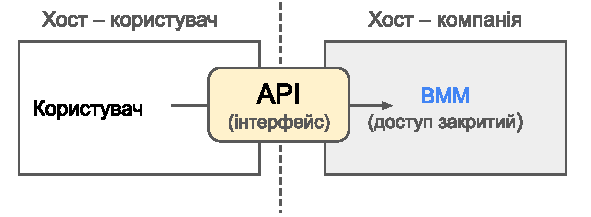
\includegraphics[width=0.8\textwidth]{closed_source_llm.pdf}
    \caption{Закриті ВММ доступні через API, внутрішні деталі яких приховані від користувача.}
    \label{fig:closed_source_llm_ua}
\end{figure}

\paragraph{Моделі з відкритим кодом}

Відкриті ВММ надають змогу отримати повний доступ до архітектури та параметрів моделі (кількість шарів, нейронів, ваги зв'язків і тд.), забезпечуючи прозорість і можливість для проведення тонкого налаштування на локальному пристрої, як це зображено на рис.~\ref{fig:open_source_llm_ua}. Для їхнього навчання або тонкого налаштування можуть знадобитися великі обчислювальні ресурси, однак за рахунок доступності та детальних описів моделей, вони нерідко є основним вибором при проведенні дослідницької роботі та експериментів.

\begin{figure}[h]
    \centering
    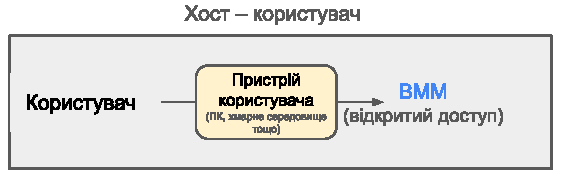
\includegraphics[width=0.8\textwidth]{open_source_llm.pdf}
    \caption{Відкриті ВММ дозволяють доступ до коду та архітектурних деталей, сприяючи локальному експериментуванню та донавчанню.}
    \label{fig:open_source_llm_ua}
\end{figure}

\subsection{Підготовка моделей для локального запуску експериментів}

Для проведення експериментів використовувалися версії моделей GPT-4 (Turbo, 4o-mini), LLaMA (2, 3, 3.1), Mixtral, Qwen (2, 2.5) -- у кількох розмірах (-7B, -8B, -13B, -70B, -8x7B, -405B) та специфікаціях (-Math, -Instruct, -Chat), які показали різні результати роботи з обробкою математичних комбінаторних задач.

Для моделей у відкритому доступі було використано їхні квантовані копії задля оптимізації використання ресурсів при локальному запуску моделей. Це дозволило зменшити обсяг необхідної пам'яті та прискорити обчислення без значної втрати точності.

Під час роботи для проведення експериментів з відкритими моделями використовувалися графічні відеокарти Nvidia Quadro RTX 8000\footnote{\url{https://www.nvidia.com/content/dam/en-zz/Solutions/design-visualization/quadro-product-literature/quadro-rtx-8000-us-nvidia-946977-r1-web.pdf}.} з 48 ГБ оперативної пам’яті та Nvidia A100\footnote{\url{https://www.nvidia.com/content/dam/en-zz/Solutions/Data-Center/a100/pdf/nvidia-a100-datasheet-us-nvidia-1758950-r4-web.pdf}.} з 80 ГБ оперативної пам’яті. Хоча пам'ять не була повністю зайнята під час експериментального процесу, видно, що GPU-Util була завантажена на 100\% (Рисунок \ref{fig:gpu_util}), що свідчить про ``вузьке місце'' обробки даних під час виконання кількох екземплярів ВММ локально на одному GPU.

Задля оптимізації та більш ефективної роботи відеокарти та створення ефективного процесу роботи з даними рекомендується використовувати кілька окремих графічних карт та об'єднувати у спільну мережу, наприклад, за допомогою технології PARCS-JAVA \cite{Anisimov2005}, які можуть дозволити проведення роботи систем без перевантаження Util-процесів.

Крім цього, результати досліджень, які представлені у статті \cite{vlasenko2019methodology}, доводять, що використання методики визначення опорної матриці моніторингу домену управління дозволяє оптимізувати інтервали опитування мережевих елементів. Зокрема, завдяки побудові дерева мережі з використанням теорії графів та методу послідовного зменшення невідомих для розв’язання системи лінійних нерівностей було можливе визначення мінімальних значень періодів моніторингу, які запобігають перевантаженню мережі службовим трафіком. Інтеграція цих підходів до експериментальної частини дослідження сприяла більш ефективному розподілу навантаження на графічну карту та оптимізації використання апаратних ресурсів.

\begin{figure}
    \centering
    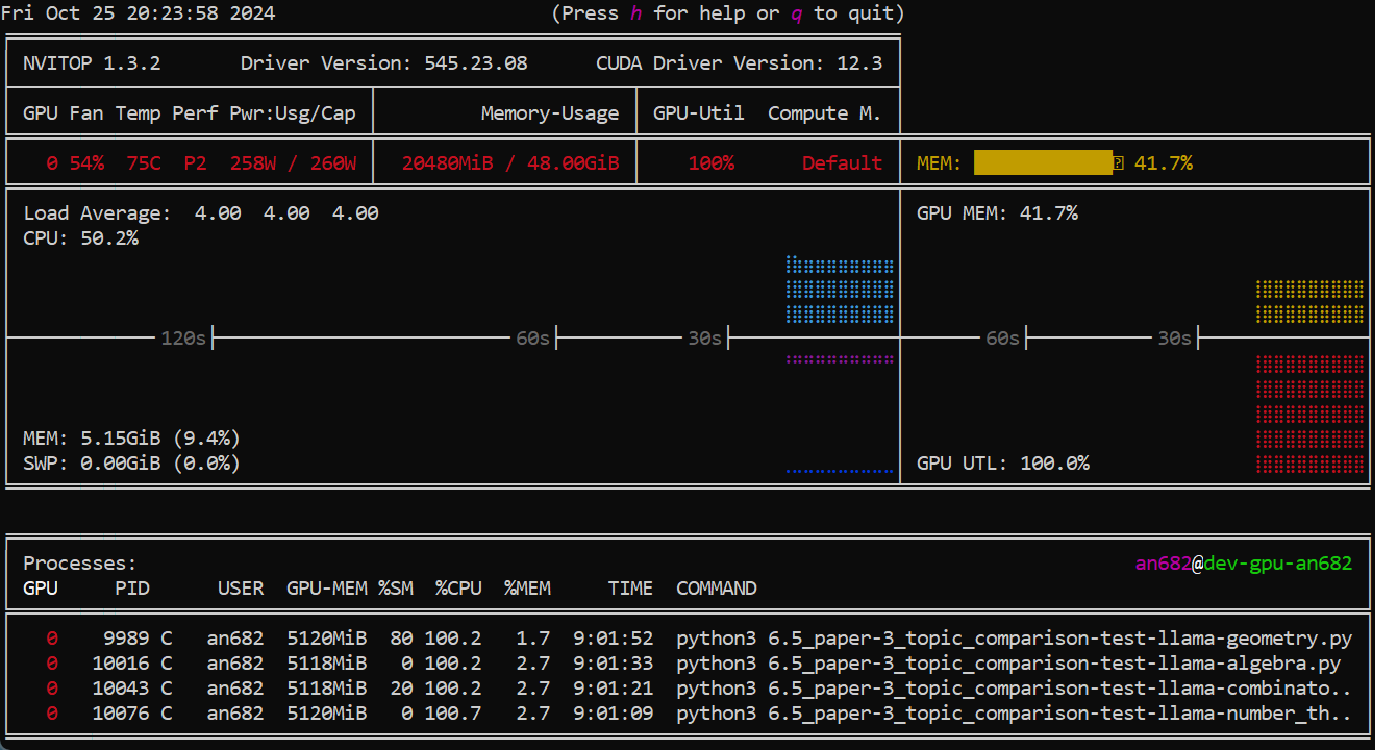
\includegraphics[width=0.9\textwidth]{data/gpu_util.pdf}
    \caption{Кілька процесів, що виконуються на графічній відеокарті, але завантажують роботу процесора на 100\%, чим сповільнюють швидкість виконання обчислень.}
    \label{fig:gpu_util}
\end{figure}

\subsection{Використання API}

Для роботи з закритими моделями використовується прикладний програмний інтерфейс (API, Application Programming Interface).

У експерименті використовувалися закриті моделі \texttt{GPT-4-Turbo-preview-v1106} та \texttt{GPT-4o-mini-2024-07-18}, які завдяки API дозволяють налаштовувати параметри без необхідності локального розгортання. 

Це забезпечує зручний інтерфейс для інтеграції моделей в експериментальне середовище.

Для проведення експерименту з \texttt{LLaMA-3.1-405B-Instruct} використовувалася також відкрита ВММ LLaMA 3.1 \cite{grattafiori2024llama3herdmodels}, яка містить близько 405 млрд. параметрів. Оскільки ця модель вимагає значної кількості додаткової пам’яті для роботи, задля запуску моделі та обробки запитів було використано хмарний сервіс Lepton AI\footnote{\url{https://www.lepton.ai/}.}, на якому відповідна модель зберігалася у квантованому вигляді.

Повний перелік моделей, використаних у експериментальній частині дослідження, наведено в Додатку~\fullref{sec:models-tested}.

\subsection{Приклад завантаження мовної моделі}

Робота з ВММ передбачає вибір та розгортання відповідних моделей. Ресурс Hugging Face\footnote{\url{https://huggingface.co/}.} є одним з найбільш поширених ресурсів для завантаження різноманітних ВММ. При виборі моделей слід звернути увагу на необхідну кількість оперативної пом'яти для роботи з моделлю. Багато моделей представлені на ресурсі мають їхні квантовані версії, які потребують менше оперативної пам'яті для роботи з ними. Наприклад, мовна модель LLaMA-3.1-8B, яка має близько 8 млрд параметрів, у 16-бітному вигляді потребує 16 ГБ оперативної пам'яті для виведення результатів, тоді як 8-бітна квантована версія -- лише 8 ГБ, але матиме меншу точність. Детальніше про квантування моделей у наступному розділі~\fullref{sec:quatisation}).

Нижче наведено фрагмент коду мовою Python для запуску та виконання запитів з моделлю LLaMA-2-70b-Chat (квант. GGUF) на віртуальній машині:
\begin{lstlisting}[language=python, breaklines=true]
#!/bin/python
import os
import sys
from termcolor import colored
from llama_cpp import Llama

MODEL_PATH = "models/llama-2-70b-chat.Q4_K_M.gguf"

MAX_TOKENS = 2048

def run_console_app():
    if not os.path.isfile(MODEL_PATH):
        print(f"Error: Invalid model path '{MODEL_PATH}'")
        sys.exit(1)

    llm = Llama(model_path=MODEL_PATH, n_gpu_layers=-1)

    print(colored("\n## Welcome to the Llama Console App! ##\n", "yellow"))
    print("Enter your prompt (or 'q' to quit):")

    while True:
        user_input = input("> ")
        if user_input.lower() == 'q':
            print("Exiting...")
            break

        user_input = f"Q: {user_input} A:"
        print(colored("Processing...", "yellow"))

        try:
            output = llm(user_input, max_tokens=MAX_TOKENS, stop=["Q:"], echo=True)

            choices_text = output["choices"][0]["text"]
            choices_text = choices_text.replace(user_input, "").strip()
            formatted_text = colored(choices_text, "green")
            print(f"\n{formatted_text}\n")
        except Exception as e:
            print(f"Error: Failed to generate response. {str(e)}")

if __name__ == '__main__':
    run_console_app()
\end{lstlisting}

Приклад вихідного тексту:
\begin{lstlisting}[language=JSON, breaklines=true]
   {"content":  Solve the following mathematical problem:
                You have 3 green apples and 5 red apples.
                How many green objects do you have?}
\end{lstlisting}


%%%%%%%%%%%%%%%%%%%%%%%%%%%%%%%%%%%%%%%%%%%%
\section{Квантування моделей}
\label{sec:quatisation}

Зі зростанням популярності інтелектуальних мобільних пристроїв та високими обчислювальними витратами моделей на базі нейронних мереж, з’явилася нагальна потреба в ефективних і точних схемах взаємодії з такими моделями безпосередньо на кінцевому пристрої. Одним зі способів розв’язання цієї проблеми є \emph{квантування моделей} -- техніка, що дає змогу зменшити обчислювальні витрати та споживання пам’яті завдяки переходу на низькорозрядні типи даних.

\subsection{Теоретичні відомості процесу квантування}

Ідея квантування полягає у стисканні моделей таким чином, аби можна було виконувати обчислення з меншими витратами ресурсів, за потреби з використанням виключно цілочисельної арифметики. Така оптимізація особливо корисна, коли апаратне забезпечення (наприклад, мобільні процесори чи мікроконтролери) не мають вбудованих реалізації для виконання числових операцій для чисел з рухомою комою.

Загалом квантування дозволяє (1) суттєво зменшити використання пам’яті моделі, (2) збільшити швидкість обчислень і (3) зберегти корисний рівень ефективності моделі. У результаті застосування низькорозрядних типів, наприклад \texttt{int8} або \texttt{float16}, на практиці можна досягнути більш економного виведення результатів при наближенні точності до початкової.

У квантованих моделях часто спостерігається зростання розрідженості, про яку згадувалося раніше, коли значна кількість параметрів може бути перетворена на нуль. Відповідно з’являється можливість додатково пришвидшити обчислення, не оброблюючи нулеві значення.

\paragraph{Наївне квантування та метод K-means}

Для демонстрації ключових підходів квантування варто розглянути два методи. \emph{Наївне квантування (Naive quantisation)} рівномірно знижує точність усіх параметрів, що можна уявити як розбиття простору на рівні за розміром ``клітинки''. Таке ділення не є рівномірним за кількістю відповідних елементів моделі, та в окремих ділянках може призвести до втрати інформації.

Натомість \emph{K-means квантування (K-means quantisation)} виконує поділ на кластери відповідно до фактичного розташування точок, забезпечуючи точніше представлення значень. Кожній точці (вазі) призначається найближчий центроїд у просторі. Завдяки цьому можна краще зберегти основні параметри моделі.

Приклад різниці між даними підходами показано на рис.~\ref{fig:quantisation}.

\begin{figure}[h]
    \centering
    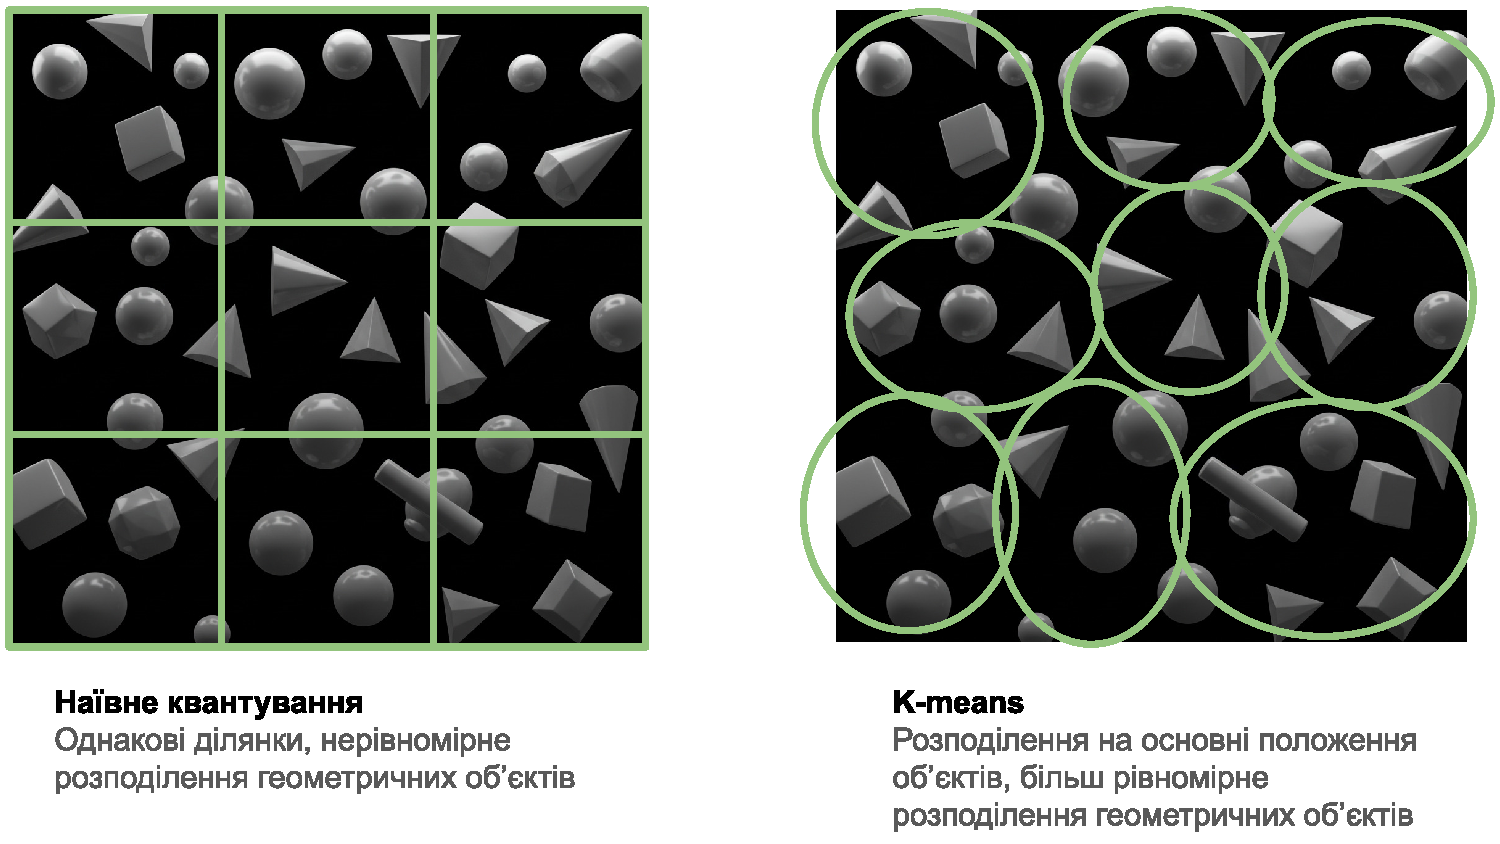
\includegraphics[width=0.8\textwidth]{quantisation_example.pdf}
    \caption{Схематичне відображення відмінностей між наївним квантуванням (ліворуч) та квантуванням за допомогою K-means (праворуч).}
    \label{fig:quantisation}
\end{figure}

\subsection{Квантування при роботі з типами даних}

Квантування зазвичай супроводжується переходом від \texttt{float32} до форматів нижчої розрядності, наприклад \texttt{float16}, \texttt{bfloat16}, \texttt{int8} тощо. Зниження числа бітів зменшує пам’ять для зберігання та спрощує обчислення. Водночас для операцій на кшталт множення потрібно мати тип накопичення з більшою розрядністю (\texttt{int32}, \texttt{float32}), щоб уникнути надто грубого заокруглення значень.

Одним з прикладів переходу є \texttt{float32} $\rightarrow$ \texttt{float16}. Ці формати є сумісними за схемою числа з рухомою комою, але \texttt{float16} має менший динамічний діапазон і може спричинити до проблем з обчисленнями занадто малих або занадто великих чисел. Проте для більшості обчислень у нейронних мережах цього діапазону достатньо.

Складнішим є перехід \texttt{float32} $\rightarrow$ \texttt{int8}, де відображення відбувається в дискретний простір, що охоплює лише 256 значень. Для цього часто використовують \emph{афінне квантування (affine quatisation)}:
\begin{equation}
x = S \cdot (x_q - Z).
\end{equation}

Тут $x$ -- початкове (floating) значення, $x_q$ -- квантоване \texttt{int8}, а $S$ і $Z$ відповідають за масштаб і нульову точку. Процес супроводжується заокругленням:
\begin{equation}
x_q = \text{round}\!\bigl(x/S + Z\bigr),
\end{equation}

та, за потреби, обрізанням вхідних значень, що виходять за встановлений діапазон. Кілька деталей стосовно навчання моделей після квантування описано у роботі~\cite{jacob2017quantizationtrainingneuralnetworks}.

\paragraph{Квантування за допомогою методу K-means}

У багатьох експериментальних задачах, зокрема для відкритих мовних моделей, використовують \emph{K-means Quantisation} з бібліотекою \texttt{llama.cpp}. Завдяки такому підходу, моделі ефективніше зберігають свої можливості й можуть набагато швидше працювати локально на звичайних пристроях. Наприклад, при квантуванні за допомогою \texttt{llama.cpp} тип квантування Q4\_K\_M значить:
\begin{itemize}
    \item {Q} -- квантування (Quantisation),
    \item {4} -- використання 4 біт на параметр,
    \item {K} -- кластеризація параметрів методом K-means,
    \item {M} -- розмір моделі після квантування (наприклад, Medium).
\end{itemize}

\subsection{Формат GGUF}

Квантовані версії моделей зберігаються у окремому файлі. Одним з поширених на даний момент форматів з є \emph{GGUF} (Generic GPT Unified Format). Раніше нейронні мережі зберігали у широковживаних форматах \texttt{.pb} для TensorFlow, \texttt{.pt} / \texttt{.pth} для PyTorch, \texttt{ONNX} для обміну між фреймворками, однак вони зазвичай: (1) зберігали повну точність \texttt{float32}, (2) не були зосереджені на квантуванні та (3) не враховували специфіки великих мовних моделей.

Поява формату GGML стала першим кроком у напрямку зниження точності до \texttt{int8} чи \texttt{int4}, що відчутно скоротило розміри файлу і надало можливість запуску великих моделей на кінцевих пристроях. Формат GGUF продовжив цей напрямок, але додав ширші можливості з управління метаданими, підтримку більших моделей (понад 100 ГБ у розмірі) і поліпшений опис архітектури.

Зокрема, GGUF призначений для генеративних моделей зі значною кількістю параметрів. Він дає змогу задати різні рівні квантування (4-біт, 8-біт тощо) і зберігати детальнішу інформацію моделі (параметри квантування, архітектуру, схему токенізації). З погляду виведення результатів це робить запуск моделей більш ефективним, оскільки всі потрібні метадані вбудовані безпосередньо у структуру файлу. Приклад структури файлу у форматі GGUF зображено на рис.~\ref{fig:gguf_architecture}.

\begin{figure}[h]
    \centering
    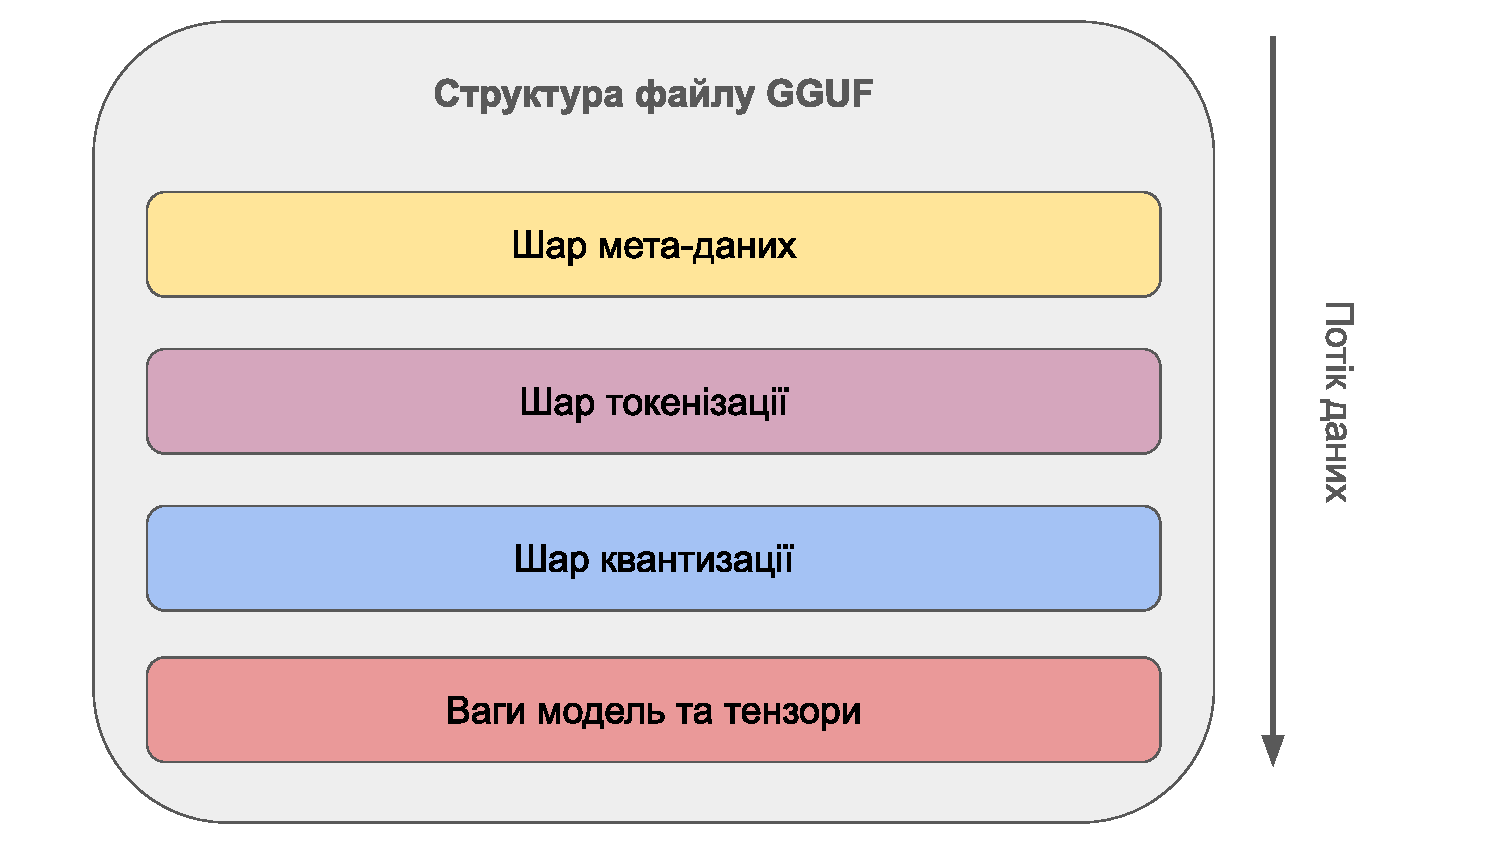
\includegraphics[width=0.8\textwidth]{gguf_architecture.pdf}
    \caption{Приклад структури файлу у форматі GGUF (умовне ілюстративне зображення).}
    \label{fig:gguf_architecture}
\end{figure}

На практиці застосування 4-бітної квантизації у форматі GGUF дає змогу знизити вимоги до оперативної пам’яті більш ніж утричі. Наприклад, для моделі LLaMA-3.1-8B зменшуючи її обсяг із 16 ГБ до приблизно 4.5 ГБ. Це дозволяє запускати більші моделі на пристроях із обмеженими ресурсами. Щодо швидкодії, залежно від конкретної реалізації та апаратного забезпечення, швидкість генерації тексту відповідно може пришвидшитися у 2-3 рази. Завдяки цим вдосконаленням великі моделі можна ефективно використовувати на пристроях з обмеженими обчислювальними ресурсами (edge-AI, мобільні системи), а також у середовищах, де є потреба в економному розподілі обладнання.

Таким чином, квантування моделей -- важливий інструмент оптимізації сучасних мовних моделей. Методи на кшталт наївного квантування, K-means квантованих схем і використання низькорозрядних типів (\texttt{float16}, \texttt{int8}, \texttt{int4}) допомагають суттєво зменшити розмір і прискорити роботу моделей із незначними втратами в точності. Формати GGML та GGUF, які є поширеними у спільноті дослідників, демонструють, як можна системно впровадити квантування і зробити великі мовні моделі більш доступними та гнучкими для різноманітних застосунків.

\subsection{Характеристики моделей використаних у експериментуванні}
\label{sec:models-tested}

У таблиці~\ref{tab:models-tested} представлено детальний перелік моделей, використаних у експериментальній частині дослідження. Усі моделі об'єднані у спільну таблицю для зручного порівняння їхніх характеристик.

\begin{figure}[!ht]
    \captionof{table}{Специфікації моделей, використаних у експерименті.}
    \label{tab:models-tested}
    \renewcommand{\arraystretch}{1.2}
    \resizebox{\textwidth}{!}{%
    \begin{tabular}{|c|l|c|c|c|p{2.5cm}|p{3cm}|l|l|}
        \hline
        \textbf{no.} & \textbf{Модель} & \textbf{Параметри} & \textbf{Кв.} & \textbf{Метод квант.} & \textbf{Довж. конт. вікна} & \textbf{Дата оновлення знань} & \textbf{Доступ} & \textbf{Розробник} \\ \hline

        1 & LLaMA-2-7B-Chat & 7 млрд & \ding{51} & Q4\_K\_M & 4k & Липень 2023 & Відкритий код & Meta \\ \hline

        2 & LLaMA-2-13B-Chat & 13 млрд & \ding{51} & Q4\_K\_M & 4k & Липень 2023 & Відкритий код & Meta \\ \hline
                
        3 & LLaMA-2-70B-Chat & 70 млрд & \ding{51} & Q4\_K\_M & 4k & Липень 2023 & Відкритий код & Meta \\ \hline

        4 & Llama-3-8B-Instruct & 8 млрд & \ding{51} & Q4\_K\_M & 128k & Грудень 2023 & Відкритий код & Meta \\ \hline
        
        5 & LLaMA-3.1-70B-Instruct & 70.6 млрд & \ding{51} & Q4\_K\_M & 128k & Грудень 2023 & Відкритий код & Meta \\ \hline

        6 & LLaMA-3.1-405B-Instruct & 405 млрд & \ding{55} & н/д & 128k & Грудень 2023 & API & Meta \\ \hline

        7 & Mixtral-8x7B & 56 млрд & \ding{51} & Q4\_K\_M & 32k & н/д & Відкритий код & Mistral AI \\ \hline  
                        
        8 & Mixtral-8x7B-Instruct & 56 млрд & \ding{51} & Q4\_K\_M & 32k & н/д & Відкритий код & Mistral AI \\ \hline

        9 & Mathstral-7B & 7.25 млрд & \ding{51} & Q4\_K\_M & 32k & н/д & Відкритий код & Mistral AI \\ \hline
        
        10 & Qwen2-7B-Instruct & 7 млрд & \ding{51} & Q4\_K\_M & 128k & н/д & Відкритий код & Alibaba Cloud \\ \hline
        
        11 & Qwen2-Math-7B & 7 млрд & \ding{51} & Q4\_K\_M & 128k & н/д & Відкритий код & Alibaba Cloud \\ \hline

        12 & Qwen2.5-Math-7B & 7.62 млрд & \ding{51} & Q4\_K\_M & 128k & н/д & Відкритий код & Alibaba Cloud \\ \hline

        13 & GPT-4-Turbo-preview-v1106 & н/д & \ding{55} & н/д & 128k & Квітень 2023 & API & OpenAI \\ \hline
        
        14 & GPT-4o-mini-2024-07-18 & н/д & \ding{55} & н/д & 128k & Жовтень 2023 & API & OpenAI \\ \hline
        
    \end{tabular}%
    }
\end{figure}

Детальний опис моделей та відповідні файли квантованих версії можна знайти у Додатку~\fullref{sec:models-tested-links}.

%%%%%%%%%%%%%%%%%%%%%%%%%%%%%%%%%%%%%%%%%%%%
\section{Тестування моделей задачами з різних математичних розділів}

Було досліджено ефективність моделей у розв'язанні задач з наступних математичних розділів: алгебра, геометрія, теорія чисел, комбінаторика. Було відібрано 8,000 задач з початкового набору даних NuminaMath-TIR \cite{numina_math_7b}, який містить 72,540 задач та проведено аналіз точності моделей у кожному розділі згідно методу описаного у роботі \cite{nikolaiev2024comparison}. 

Для проведення тестування були використані відкриті моделі Llama-3.1-8B-Instruct, Qwen2.5-Math-7B, Mathstral-7B та закрита модель GPT-4o-mini. Обчислення виконувалися на графічній відеокарті Nvidia Quadro RTX 8000. Результати експерименту описані у наступному розділі дисертаційної роботи.

\section{Тестування моделей на власному наборі задач}

\subsection{Комп'ютерні ресурси для обчислення}

У лаштунках наукової роботи було проведено експериментальне дослідження здатності моделей розв'язувати комбінаторні задачі з лінгвістичними та структурними змінами в умовах задач. Було виконано порівняння роботи моделей GPT-4, LLaMA (версії 2 та 3.1), Mixtral, які потім було порівняно з результатами людей-експертів \cite{nikolaiev2024can}.

У таблиці~\ref{tab:llm_computation} наведено загальний обсяг оброблених запитів та час на обробку. Тестування відбувалося у три серії, які виконувалися з оновленою версією набору даних та відповідних моделей кожна з яких відділена подвійною лінію у таблиці ~\ref{tab:llm_computation}.

Тестування моделей виконувалося у вигляді звичайного запиту у вигляді задачі разом з додатковою інструкцією або лише задачі без додаткової інструкції. Загальна кількість запитів склала близько 30 тис. на експериментальних серіях 1-2 та ще 6 тис. на третій серії експериментів, разом -- близько 36 тис. запитів. Кожен запит ініціювався у вигляді окремого діалогу з моделлю. На обчислення за допомогою GPU RTX8000, A100, а також ресурсів від Open AI було витрачено разом близько 225 годин роботи моделей. Виконання запитів Open AI виконувалося швидко, з приблизною вартістю близько \$12.60 за 1375 одиниць запитів (з урахуванням попереднього тестування).

\begin{figure}[!ht]
    \centering
    \captionof{table}{Результати експериментів з ВММ.  
    Види варіацій: A = звичайна, B = математична, C = надлишкова, D = параметризована, E = лінгвістичне заплутування.}  
    \label{tab:llm_computation}
    \renewcommand{\arraystretch}{1.2}
    \resizebox{\textwidth}{!}{%
    \begin{tabular}{|l|l|c|c|c|c|c|c|l|}
    \hline
    \multirow{2}{*}{\textbf{Модель}} & \multirow{2}{*}{\textbf{Додаткова інструкція (англ.)}} & \multicolumn{5}{c|}{\textbf{Варіації задач}} & \multirow{2}{*}{\textbf{Час оброб.}} & \multirow{2}{*}{\textbf{GPU}} \\
    \cline{3-7}
    & & A & B & C & D & E &  &  \\
    \hline
    \hline

    LLaMA-2-7B/13B/70B & <None> & $25 \times 10$ & $25 \times 10$ & - & - & $25 \times 10$ & 10 год & RTX8000 \\
    LLaMA-2-7B/13B/70B & Give a short answer. & $25 \times 10$ & $25 \times 10$ & - & - & $25 \times 10$ & 10 год & RTX8000 \\
    LLaMA-2-7B/13B/70B & The answer is & $25 \times 10$ & $25 \times 10$ & - & - & $25 \times 10$ & 10 год & RTX8000 \\
    LLaMA-2-7B/13B/70B & The answer (arabic numerals) is & $25 \times 10$ & $25 \times 10$ & - & - & $25 \times 10$ & 10 год & RTX8000 \\
    LLaMA-2-7B/13B/70B &  Let’s think step by step. & $25 \times 10$ & $25 \times 10$ & - & - & $25 \times 10$ & 10 год & RTX8000 \\
    \hline
    \hline

    LLaMA-2-7B/13B/70B & <None> & $25 \times 10$ & $25 \times 10$ & $25 \times 10$ & $25 \times 10$ & $25 \times 10$ & 27.5 год & RTX8000 \\
    LLaMA-2-7B/13B/70B &  The short and correct answer. & $25 \times 10$ & $25 \times 10$ & $25 \times 10$ & $25 \times 10$ & $25 \times 10$ & 28.5 год & RTX8000 \\
    LLaMA-2-7B/13B/70B &  Give me a short expression as an answer. & $25 \times 10$ & $25 \times 10$ & $25 \times 10$ & $25 \times 10$ & $25 \times 10$ & 28 год & RTX8000 \\
    \hline
    Mixtral-8x7B-/Instruct & <None> & $25 \times 10$ & $25 \times 10$ & $25 \times 10$ & $25 \times 10$ & $25 \times 10$ & 12.5 год & RTX8000 \\
    Mixtral-8x7B-/Instruct & The short and correct answer. & $25 \times 10$ & $25 \times 10$ & $25 \times 10$ & $25 \times 10$ & $25 \times 10$ & 9.5 год & A100 \\
    Mixtral-8x7B-/Instruct & The short and correct answer. & $25 \times 10$ & $25 \times 10$ & $25 \times 10$ & $25 \times 10$ & $25 \times 10$ & 12.5 год & RTX8000 \\
    \hline
    \hline

    LLaMA-3.1-70B-Instruct & <None> & $25 \times 10$ & $25 \times 10$ & $25 \times 10$ & $25 \times 10$ & $25 \times 10$ & 15 год & RTX8000 \\
    LLaMA-3.1-70B-Instruct & The short and correct answer is & $25 \times 10$ & $25 \times 10$ & $25 \times 10$ & $25 \times 10$ & $25 \times 10$ & 15 год & RTX8000 \\
    \hline
    Mixtral-8x7B-Instruct & <None> & $25 \times 10$ & $25 \times 10$ & $25 \times 10$ & $25 \times 10$ & $25 \times 10$ & 12.5 год & RTX8000 \\
    Mixtral-8x7B-Instruct & The short and correct answer is & $25 \times 10$ & $25 \times 10$ & $25 \times 10$ & $25 \times 10$ & $25 \times 10$ & 12.5 год & RTX8000 \\
    \hline
    GPT-4-Turbo & <None> & $25 \times 5$ & $25 \times 5$ & $25 \times 5$ & $25 \times 5$ & $25 \times 5$ & 1-2 год & API \\
    GPT-4-Turbo & The short and correct answer is & $25 \times 5$ & $25 \times 5$ & $25 \times 5$ & $25 \times 5$ & $25 \times 5$ & 1-2 год & API \\
    \hline
    \hline
    
    \multicolumn{2}{|r|}{\textbf{Загально:}} & \multicolumn{5}{|r|}{\textbf{36,250 запитів}} & \textbf{225.5 год} & - \\
    \hline
    \end{tabular}%
    }
\end{figure}

\subsection{Критерії оцінювання відповідей моделей}

Задля перевірки результатів роботи моделей було розроблено критерії оцінювання, які враховують точність, повноту та логічну послідовність наведених розв'язань. Це забезпечує об'єктивність та порівнянність результатів між різними моделями та з результатами людей. Схема включає бінарну оцінку правильності розв'язків та аналіз проміжних кроків генерації розв'язання.

Це досягається за рахунок набору правил, які застосовувалася для надання оцінок відповідям моделей. Оскільки експериментування відбувалося з математичними комбінаторними задачами, у деяких випадках люди та ВММ повертають відповіді не у числовій формі, а як комбінаторну формулу з використанням біномів, факторіалів та інших комбінаторних символьних представлень, наприклад, відповіді у вигляді \(C(11, 2) = 55\) -- також приймалися, якщо вони еквіваленті числовому значенню правильної відповіді на задачу. Нижче перелічено набір правил, які були застосовані у схемі оцінювання, включаючи випадки ``сірої зони'', коли відповідь моделі можна трактувати по-різному. Критерії оцінювання наведені нижче.

Критерії оцінювання за надання ``1'' (розв'язок правильний):
\begin{enumerate}
    \item \textit{Бал: 1} -- Відповідь коротка та правильна.
    \item \textit{Бал: 1} -- На початку наведенo правильний розв'язок, навіть якщо далі слідує неправильна або нерелевантна інформація.
    \item \textit{Бал: 1} -- Наприкінці наведено правильний розв'язок, навіть якщо перед цим присутня неправильна або нерелевантна інформація.
    \item \textit{Бал: 1} -- Модель перелічує кілька варіантів розв'язку та вказує на правильний.
    \item \textit{Бал: 1} -- Модель починає з неправильного розв'язку, але потім приходить до правильного.
    \item \textit{Бал: 1} -- Комбінаторний розв'язок правильний, але модель надає наближену числову відповідь (наприклад, з використанням слів ``приблизно'', ``близько'', символу ``\(\approx\)'' тощо).
\end{enumerate}

Критерії оцінювання за надання ``0'' (розв'язок неправильний):
\begin{enumerate}
    \item \textit{Бал: 0} -- Розв'язок неправильний.
    \item \textit{Бал: 0} -- Розв'язок відсутній.
    \item \textit{Бал: 0} -- Розв'язок не містить числових або комбінаторних елементів.
    \item \textit{Бал: 0} -- Модель не завершила розв'язання та не прийшла до фінального розв'язку.
    \item \textit{Бал: 0} -- Модель перелічує кілька розв'язків (можливо, разом з правильним), але обирає неправильний або жодний.
    \item \textit{Бал: 0} -- Розв'язок був представлений у вигляді мовою програмування.
    \item \textit{Бал: 0} -- Модель має правильні кроки обґрунтування, але приходить до неправильного висновку.
    \item \textit{Бал: 0} -- Модель виконала неправильний перехід під час обрахунків; відповіді частини перетворень з'єднані знаком рівності або такими, як наприклад, ``або'', ``дорівнює'' тощо.
    \item \textit{Бал: 0} -- Розв'язок неоднозначний (не надано фінальної розв'язку).
\end{enumerate}

Схема оцінювання забезпечує детальну та об'єктивну оцінку відповідей моделей, враховуючи різні формати відповідей та можливі варіанти їх подання. Це дозволяє точно визначити правильність розв'язку, навіть якщо він представлений у незвичайній формі. Крім того, врахування ``сірої зони'' дозволяє більш гнучко перевіряти відповіді моделей, які є частково правильними або потребують додаткової інтерпретації.

\section{Генерація синтетичних варіацій комбінаторних задач}

Задля генерації задач було використано підхід описаний у роботі \cite{nikolaiev2025synth} з фінальним набором, що містив 1,000 комбінаторних задач. Даний набір даних був розширений до 5,583 задач за допомогою методів відбору даних описаних у відповідній роботі. Нижче описується послідовність кроків, які були виконані для проведення експериментальної частини дослідження з відповідними даними.

Задля проведення експериментальної частини було використано набір даних Numina-CoT \cite{numina_math_7b}, який як згадувалися раніше, містить близько 860 тис. різноманітних математичних задач.

\subsection{Генерація синтетичних варіацій задач}

Генерація синтетичних даних включає систематичну маніпуляцію з текстовими умовами задач відфільтрованого набору даних. В результаті вводиться кілька нових варіацій задач: (i) \emph{художня варіація} з заміною стилю тексту задачі у вигляді вигаданої історії; (ii) \emph{надлишкова варіація}, у який вводиться зайва числова інформація у формулювання оригінальної умови задачі; та (iii) \emph{прихована варіація}, що розміщує задачу у нерелевантному контексті. Аналогічно до переднього етапу, задля вищої точності роботи з моделями, а також оскільки вхідні дані задані англійською мовою, усі інструкції передавалися до моделей англійською мовою.

Процес генерації варіацій текстів задач відбувається на основі оригінального тексту задач за допомогою ВММ GPT-4o-mini. Модель було обрано завдяки її швидкості та ефективності роботи з технічними текстами, зокрема з темами з математики, програмування та питаннями пов'язанні із наукою. Вона призначена для вирішення складних завдань, але при цьому є ресурсоефективною, що робить її придатною для обробки великого набору даних. Модель має контекстне вікно у розмірі 128,000 токенів і зріз знань на момент жовтня 2023 року\footnote{\url{https://openai.com/index/gpt-4o-mini-advancing-cost-efficient-intelligence/}}.

Звернення до моделі відбувалися за допомогою API. У відповідному запиті до моделі було додано інструкцію про те, щоб варіації задачі зберігали математичну основу задля забезпечення однакового числового розв'язку, що є важливим для подальшого оцінювання точності згенерованих даних. Додатково у запитах до моделі було внесено інструкцію про збереження розміру варіацій задач подібним до оригіналу, але в багатьох випадках з художньою варіацією модель порушувала дану умову, що приводило до генерації більш довгих текстів задач. Середня довжина (у кількості символів) згенерованих текстів варіації задач зазначено у таблиці~\ref{tab:var_len}.

\begin{figure}
    \centering
    \captionof{table}{Середня довжина умов варіацій задач.}
    \label{tab:var_len}
    \begin{tabular}{|l|c|}
    \hline
    Варіація & Сер. к-ть символів \\
    \hline
     Оригінальна & 248 \\
     Художня & 651 \\
     Надлишкова & 303 \\
     Прихована & 320 \\
     \hline
    \end{tabular}
\end{figure}

Процес генерації синтетичних версій задач на основі оригінальних текстів виконувався за наступним запитом, де за допомогою параметру style було задано відповідну варіацію задачі:

\begin{lstlisting}[language=json, breaklines=true]
{"content": "Apply the {style} to the following mathematical 
            problem. Retain the mathematical core and keep
            the resulting statement approximately similar 
            in length. Return just the problem statement. 
            Problem: {problem_statement}"}
\end{lstlisting}

\subsection{Генерація розв'язків}

Щоб забезпечити якість міркування і покращити точність моделі у розв'язанні задач, виконувалося 2 етапи:

\begin{enumerate}
    \item Модель GPT-4o-mini використовується для розв'язання усіх варіацій задач. Для кожної варіації задачі разом з оригінальним формулюванням умови, було згенеровано математичне розв'язання за наступним запитом:
\begin{lstlisting}[language=json, breaklines=true]
{"content": "Solve the following mathematical problem. 
            Return a solution with the final numerical 
            answer at the end. Problem: 
            {problem_statement}"}
\end{lstlisting}
    
    \item Після цього зі згенерованого розв'язання вилучається числова відповідь (розв'язок). Для вилучення відповідей використовується нейромережевий метод, описаний у Розділі~\fullref{sec:problem-selection}. У деяких випадках мовна модель не змогла згенерувати розв'язання з єдиною позитивною числовою відповіддю -- у такому разі вважається, що задачу не було розв'язано моделлю.
\end{enumerate}

Таким чином, забезпечується стабільність роботи моделі з різними варіаціями задач, тоді як етап відбору та підготовки даних відбувається незалежно та виконується іншою моделлю.

\begin{figure}[!ht]
    \small
    \centering
    \captionof{table}{Детальний опис набору даних задач та їх згенерованих синтетичних варіацій.}
    \label{tab:dataset_final}
    \begin{tabular}{|p{4.5cm}|p{9cm}|}
        \hline
        \textbf{Назва поля (початкові дані з набору Numina-CoT)} & \textbf{Оригінальна задача} \\ \hline
        \texttt{problem\_id} & Унікальний ідентифікатор для кожної задачі. \\ \hline
        \texttt{source} & Джерело задачі. \\ \hline
        \texttt{problem} & Умова задачі. \\ \hline
        \texttt{solution} & Розв'язання задачі. \\ \hline
        \texttt{messages} & Дані у форматі ланцюжка думок. \\ \hline
        \texttt{answer} & Вилучений розв'язок на задачу. \\ \hline \hline
        \textbf{(згенеровані синтетичні дані)} & \textbf{Згенеровані синтетичні дані} \\ \hline
        \texttt{fictional} & Художня варіація задачі. \\ \hline
        \texttt{adversarial} & Надлишкова варіація задачі. \\ \hline
        \texttt{contdis} & Прихована варіація задачі. \\ \hline
        \texttt{original\_sol} & Розв'язання оригінальної варіації. \\ \hline
        \texttt{fictional\_sol} & Розв'язання художньої варіації. \\ \hline
        \texttt{adversarial\_sol} & Розв'язання надлишкової варіації. \\ \hline
        \texttt{contdis\_sol} & Розв'язання прихованої варіації. \\ \hline
        \texttt{original\_ans} & Вилучений розв'язок оригінальної варіації. \\ \hline
        \texttt{fictional\_ans} & Вилучений розв'язок художньої варіації. \\ \hline
        \texttt{adversarial\_ans} & Вилучений розв'язок надлишкової варіації. \\ \hline
        \texttt{contdis\_ans} & Вилучений розв'язок прихованої варіації. \\ \hline
    \end{tabular}
\end{figure}

\subsection{Структура зберігання синтетичного набору даних}

Кінцевий набір синтетичних даних містить 22,332 задач (з відібраного початкового набору 5,583 задач) об'єднані у колекції, що містять інформацію про кожну з задач: оригінальна, художня варіація, надлишкова варіація та прихована варіація. Кожна задача у колекції задач містить детальне розв'язання та кінцевий числовий розв'язок до неї. Детальний опис атрибутів до кожної колекції задач надано у таблиці~\ref{tab:dataset_final}. Структура розширеного набору даних відформатована та збережена Parquet і JSON для ефективної роботи мовою програмування Python 3.11. Приклад задачі наведено у Додатку~\fullref{sec:problems-synthetic}.

% Треба додати лінк на датасет (але спочатку його треба створити).

\subsection{Обмеження набору задач}

За рахунок того, що деякі задачі у оригінальному наборі даних дублюються, вони повторюються у отриманому комбінаторному наборі задач. Задачі не були прибрані з фінального набору даних, оскільки не зважаючи на співпадіння, їхня варіативність була іншою, тобто процес генерації приводив до унікальних версій тих самих задач, чим збагачував різноманітність синтетичного набору даних.

Також слід зазначити, що у оригінальному наборі задач Numina-CoT можливі помилки. Наприклад, для задачі із таблиці~\ref{tab:original_wrong} слідує, що відповідь на задачу 4, однак не складно перевірити, що можливих варіантів, що задовольняють умові задачі є 6 (числа $2005, 2050, 2500, 5002, 5020, 5200$). З урахуванням даного моменту слід зазначити, що згенеровані розв'язки до варіації початкової задачі могли бути неправильно оцінені на наступних етапах генерації задач.

\begin{figure}[h!]
    \centering
    \small
    \captionof{table}{Приклад задачі з оригінального набору Numina-CoT з помилковою відповіддю.}
    \label{tab:original_wrong}
    \begin{tabular}{|p{0.6\linewidth}|p{0.15\linewidth}|p{0.15\linewidth}|}
        \hline
        \textbf{Умова задачі} & \textbf{Відповідь Numina-CoT} & \textbf{Правильна відповідь} \\
        \hline
        How many different four-digit numbers can be formed by arranging the four digits in 2005? (\textit{Умова задачі українською:} Скільки різних чотирицифрових чисел можна утворити з числа 2005?) & \hlred{4 числа} & \hlgreen{6 чисел} \\
        \hline
    \end{tabular}
\end{figure}

\section{Експериментальна частина з участю людини}
\label{sec:human-experiment-set-up}

\subsection{Умови проведення експерименту}

Учасниками експерименту були українські школяри та студенти, які знайомі з темою комбінаторики та мають попередній досвід участі на математичних змаганнях. Загалом у дослідженні взяли участь 35 учасників віком від 13 до 18 років.

Експеримент організовано за допомогою латинського квадрату (Latin Square). Було сформовано 5 груп по 7 учасників в кожній групі з приблизно однаковим розподілом за середнім віком. Учасникам кожної групи було призначено один із п'яти комплектів задач. Кожен комплект містив 25 задач з рівномірно розподіленими варіаціями задач (5 задач на кожну з 5 варіацій). Задачі були перекладені з англійської на українську мову, щоб учасники могли впевнено прочитати та зрозуміти умови задачі. Кожен з учасників працював самостійно. Розподіл груп учасників та варіантів задач представлено на Рисунку~\ref{fig:packs}.

\begin{figure}
    \centering
    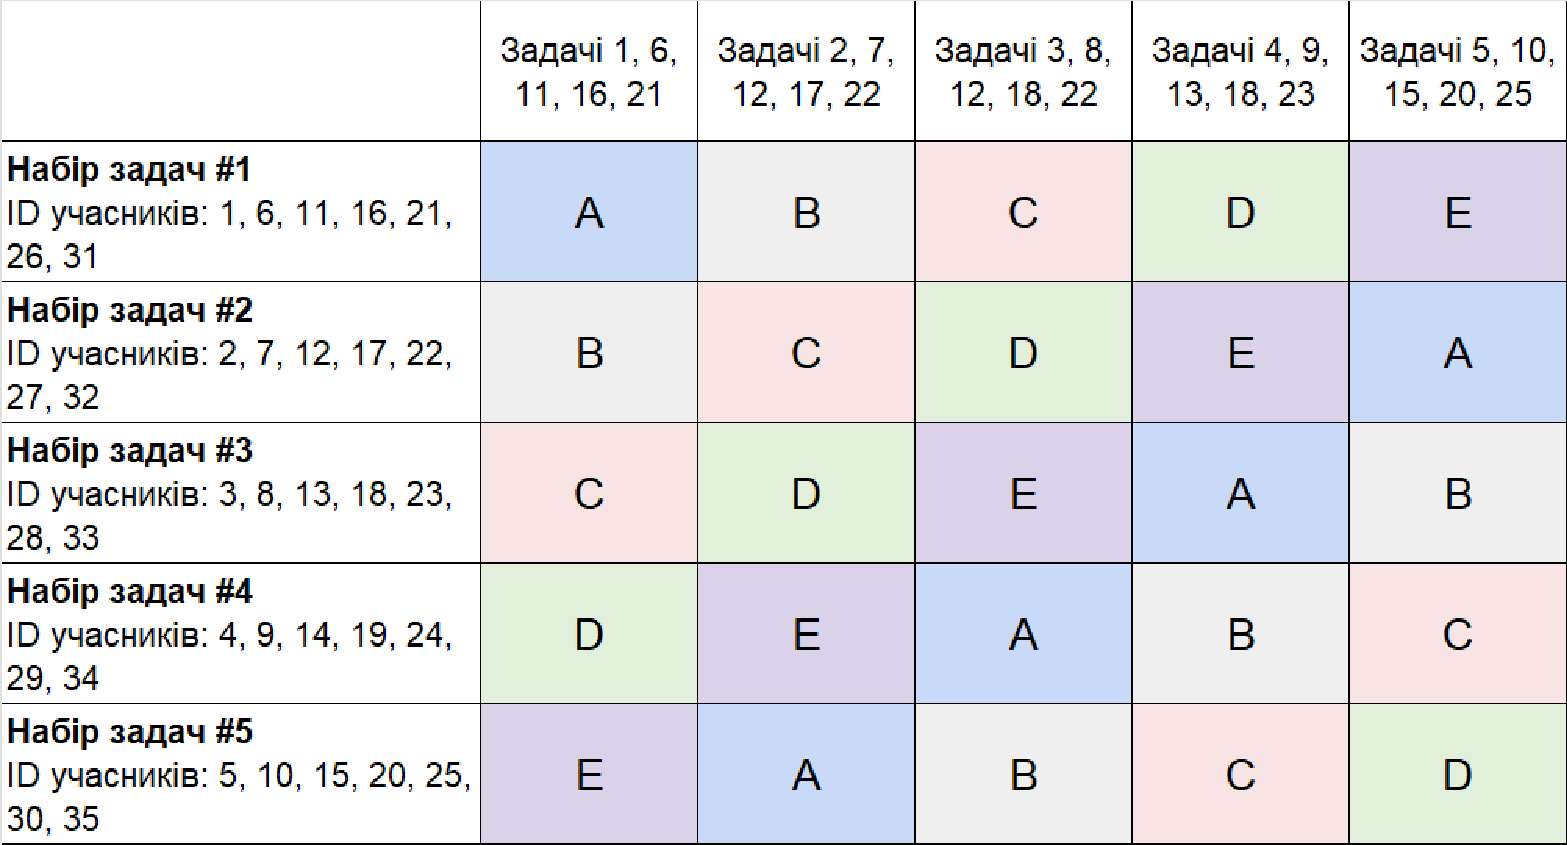
\includegraphics[width=0.8\textwidth]{packs.pdf}
    \caption{Розподіл матеріалів (задач) та учасників для проведення експериментальної частини відповідно до латинського квадрату. Букви та кольори визначають відповідні використані варіації задач: A = \hlgrey{звичайна} (сірий), B = \hlblue{математична} (блакитний), C = \hlred{надлишкова} (червоний), D = \hlgreen{параметризована} (зелений), E = \hlpurple{лінгвістичне заплутування} (фіолетовий).}
    \label{fig:packs}
\end{figure}

\subsection{Збір та підготовка даних}

Відповіді учасників були зібрані та оцінені за розробленою схемою оцінювання. Кожен учасник надавав розв'язки на задачі свого комплекту у короткій комбінаторній або числовій формі, кожен з отриманих розв'язків задач отримував оцінку 0 (неправильна) або 1 (правильна). У випадку відсутності розв'язку на певну задачу, учасник отримував оцінку 0. Враховуючи різноманітні формулювання, правильна відповідь могла бути представлена у формі комбінаторної формули, тому в деяких випадках доводилося застосовувати додаткові розрахунки під час оцінювання.

Результати між ВММ та учасниками порівнювалися наступним чином: для ВММ було обрано модель, яка продемонструвала найкращі результати роботи серед протестованих моделей, тоді як серед учасників кожної групи обиралися 5 найкращих результатів по кожній з груп, які потім разом представляли експертну оцінку.

\subsection{Умови етики для участі в експерименті}

Це дослідження було проведено як контрольований експеримент, що відбувалася відповідно до етичних стандартів залучення учасників експерименту (людей). Було залучено 35 поточних та колишніх студентів українського освітнього STEM-проекту Kvanta\footnote{\url{https://www.kvanta.xyz/}.}. Кожен учасник надав згоду з правилами участі в експерименті, для учасників молодше 16 років згоду було отримано від батьків. Експеримент оцінював математичні навички міркування на варіаціях комбінаторних задач дистанційно. Дані, які було зібрано для проведення експерименту -- вік учасників, розв'язки на переданий набір задач та час витрачений на розв'язання задач. Участь в експерименті була добровільною, і учасники були поінформовані про право відмовитися від участі в експерименті у будь-який момент. Інструкції включали загальну інформацію про кількість представлених задач, їхню складність та варіативність стилю. Грошова компенсація не передбачалася, але участь пропонувалася як навчальна можливість. Комунікація з учасниками була чіткою, підкреслюючи, що дослідження є окремим від звичайної діяльності освітнього проекту.

\subsection{Обмеження набору задач}

Основними обмеженнями запропонованого нового набору задач є:

\begin{enumerate}
    \item {Досвід учасників.} Віковий діапазон учасників складає від 13 до 18 років із медіаною у 16 років. Хоча всі учасники мають досвід участі в математичних змаганнях і знайомі з комбінаторикою, їхній досвід є різноманітним через вікову різницю, що може впливати на підготовленість до ефективного розв'язання задач у нових варіаціях. Було забезпечено рівномірний розподіл вікових відмінностей серед груп, що дозволило мінімізувати дані обмеження задля цілей дослідження.
    \item {Розмір набору даних Combi-Puzzles.} Через те, що задачі були підготовлені власноруч, отриманий набір містить 125 варіантів задач, що може не повністю відображати різноманітність сценаріїв, з якими можуть стикатися ВММ. Це обмежує загальність результатів для широких застосувань.
    \item {Якість перекладу текстів задач.} Задачі були представлені учасникам українською мовою, тоді як оригінальні задачі були підготовлені англійською. Не зважаючи на те, що було приділено окрему увагу збереженню стилістичних та інших особливостей кожної варіації задачі, отриманий переклад задач може трохи відхилятися від оригінальної форми. Зокрема задля забезпечення точності українського перекладу тверджень доступного для розуміння учасникам, вживані комбінаторні формулювання були замінені на їхні українські еквіваленти. Наприклад, формулювання ``drawing balls with replacement'' була перекладена як ``після того, як ви берете кулю, ви її повертаєте назад''. Ці адаптації мотивовані відмінностями в математичних формулюваннях текстів задач між українською та англійською мовами, які спостерігаються у математичних шкільних підручниках.
\end{enumerate}

Ці обмеження варто враховувати при інтерпретації результатів дослідження та їхнього узагальнення задля подальших напрямів розвитку та оптимізації підходів до оцінки математичної здатності великих мовних моделей.

\section{Підсумки розділу}
У цьому розділі було проведено комплексне експериментальне дослідження методів генерації математичних комбінаторних задач за допомогою великих мовних моделей, що охоплює як технічні аспекти розгортання та налаштування моделей, так і практичну оцінку їхньої здатності до синтезу та розв'язання задач. Було проведено аналіз інтерфейсів роботи з ВММ, де окремо висвітлено роботу із закритими моделями (GPT-4) через API, а також розглянуто моделі з відкритим кодом (LLaMA, Mixtral, Qwen), що використовуються локально із застосуванням їхніх квантованих копій задля оптимізації використання обчислювальних ресурсів. Детально було обговорено процес налаштування експериментального середовища, включно з демонстрацією прикладів завантаження моделей за допомогою бібліотек у Python та інженерії запитів для отримання результатів, що ілюструє практичну реалізацію роботи з моделлю, а також специфіку використання апаратного забезпечення, зокрема графічних процесорів. 

Було розглянуто методи квантування моделей, зокрема популярний для більшості сучасних бібліотек (таких як \texttt{llama\_cpp}) метод з використанням K-means, що дозволило визначити їх вплив на використання пам’яті, швидкість обчислень та точність моделі. Описано процес адаптації моделей до роботи з різноманітними типами даних, зокрема переходу від float32 до float16 і int8, з розглядом підходів до квантування та методів обчислення квантованих значень, що має суттєве значення для розгортання моделей на кінцевих пристроях із обмеженими ресурсами.

У розділі було проведено тестування моделей на синтезованому наборі даних, що включало завдання з лінгвістичними та структурними варіаціями, що дозволило оцінити їх здатність розв’язувати комбінаторні задачі з різних математичних розділів, таких як алгебра, геометрія, теорія чисел і комбінаторика. Було розроблено критерії оцінювання відповідей моделей, які враховують не лише правильність фінального результату, а й логічність проміжних кроків розв’язання, а також адаптований набір критеріїв для аналізу відповідей у разі використання комбінаторних формул. 

Крім того, було проведено розширення початкового набору даних за допомогою генерації синтетичних варіацій задач, що включали художні, надлишкові та приховані варіанти, за допомогою GPT-4o-mini. Було описано послідовність створення варіацій, генерації розв’язань та вилучення фінальних числових відповідей, що дозволило уникнути неоднозначностей і забезпечити стабільність результатів. Структура зберігання даних була оптимізована шляхом використання Parquet та JSON форматів, що сприяло зручності подальшого аналізу на досліджуваному наборі задач. 

У розділі було здійснено експериментальну частину з участю людини, у якій залучено молодих учасників, що мали попередній досвід з комбінаторикою. Було детально описано умови проведення експерименту, особливості перекладених текстів задач, збір та підготовку даних, що дозволило провести порівняння роботи ВММ із результатами учасників-експертів у контрольованому середовищі. Особлива увага приділялася забезпеченню етичних норм під час проведення дослідження, формуванню рівномірного розподілу завдань та врахуванню обмежень, пов'язаних із досвідом учасників і точностями перекладних текстів.

Таким чином, результати розділу свідчать про успішну інтеграцію сучасних великих мовних моделей для автоматизованого створення математичних комбінаторних задач, що відкриває широкі можливості для їхнього застосування як у дослідницьких, так і в практичних умовах та є актуальним для подальших удосконалень у сфері синтезу даних і покращення ефективності моделей для розв’язання математичних задач.

\chapter{Аналіз ефективності нейромережевих методів для генерації синтетичних текстів}

%%%%%%%%%%%%%%%%%%%%%%%%%%%%%%%%%%%%%%%%%%%%%%%%%%%%%%%
\section{Дослідження впливу математичних розділів задач на ефективність генерації розв'язків}

Цей підрозділ представляє статистичний аналіз ефективності розв’язання задач у різних математичних розділах на протестованих моделях. Як згадувалося раніше задачі були розподілені 4 основні математичні розділи: алгебра, комбінаторика, геометрія та теорія чисел.

Для проведення результати спочатку було отримано середню частоту правильних розв'язків моделей за різними розділами. Далі було використано статистичний критерій хі-квадрат та метод перестановок для оцінки того, чи є розподіл правильних та неправильних розв'язків між розділами статистично значущим, а також для визначення середніх показників ефективності протестованих моделей до кожного окремо розглянутого математичного розділу.

\begin{figure}[!h]
    \centering
    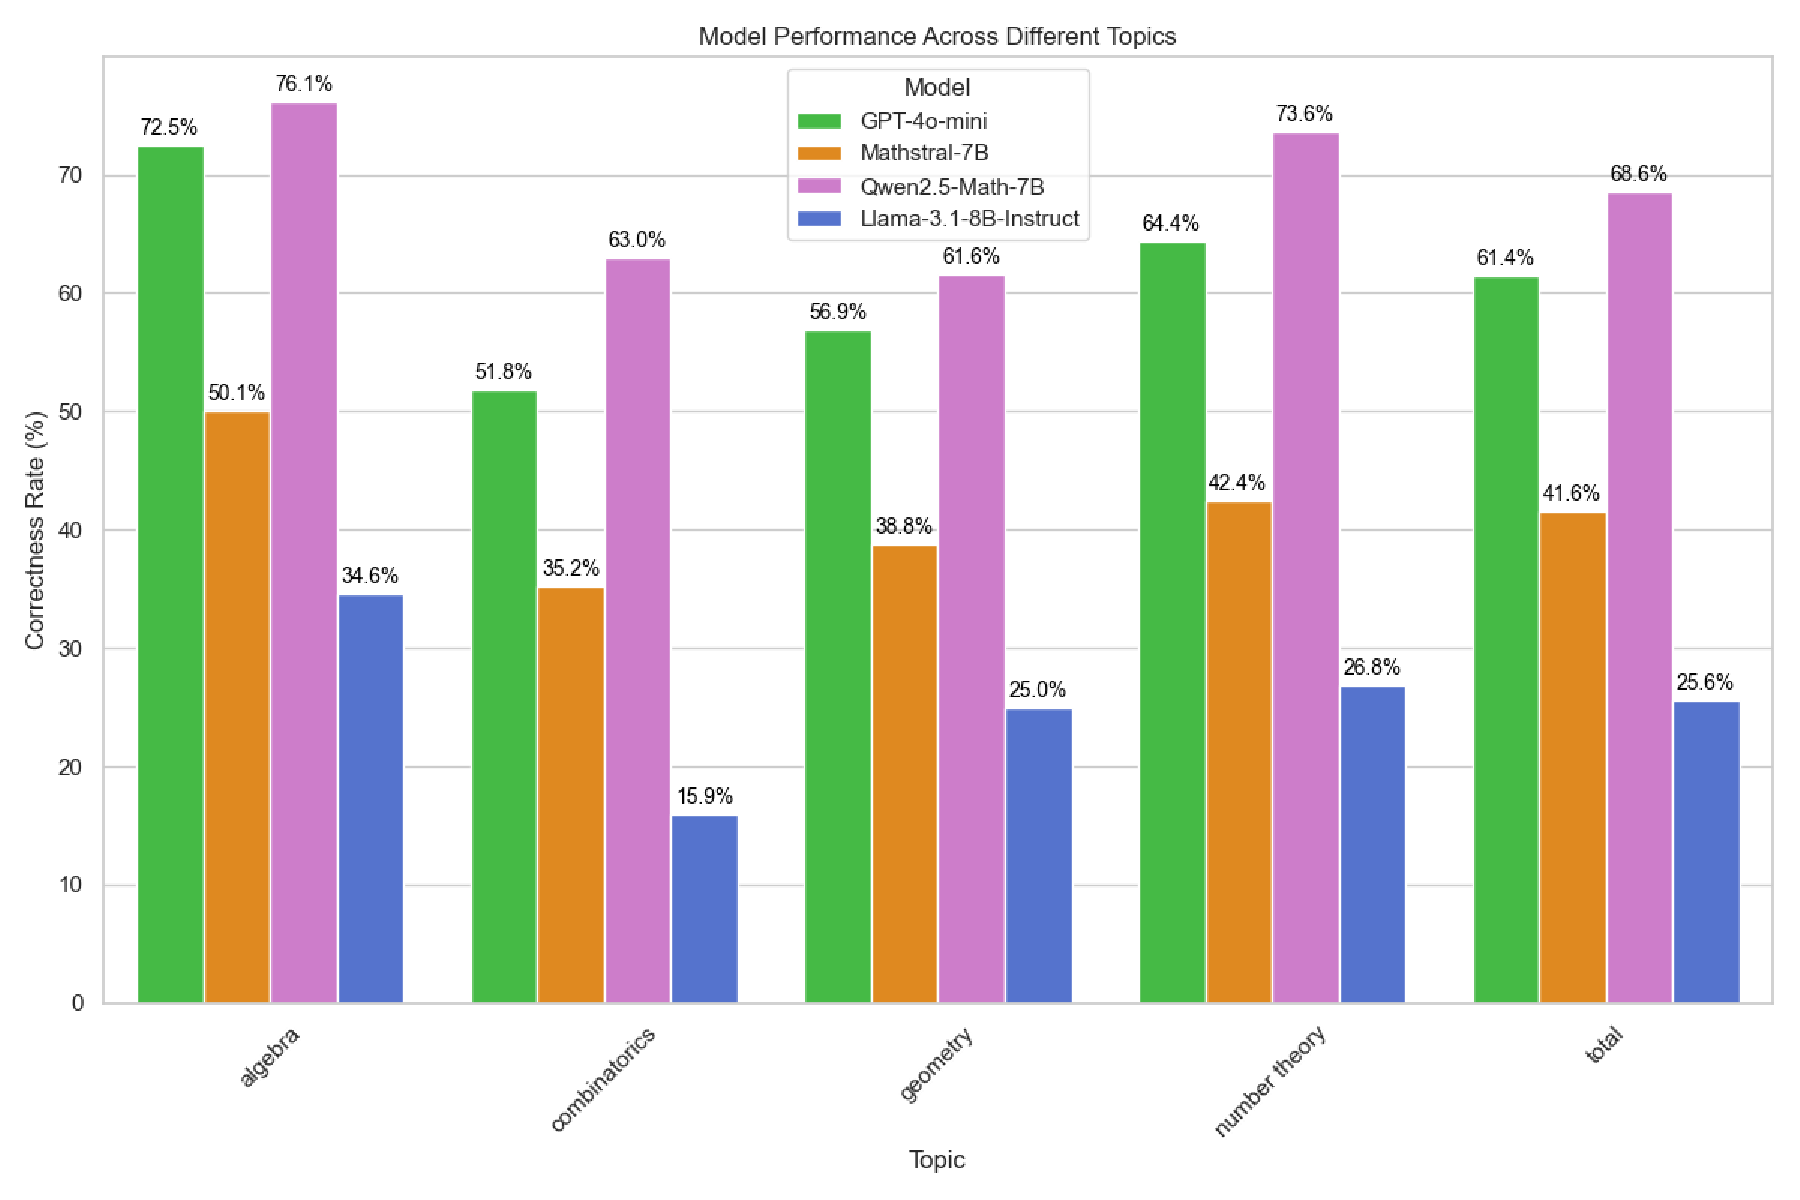
\includegraphics[width=0.9\textwidth]{correctness_rate.pdf}
    \caption{Середня точність розв'язків по різних математичних розділах моделями GPT-4o-mini (зелений), Mathstral-7B (помаранчевий), Qwen2.5-Math-7B (фіолетовий), Llama-3.1-8B-Instruct (блакитний).}
    \label{fig:correctness_rate}
\end{figure}

Загальні результати показали, що моделі досягають найкращих результатів 
з задачами у алгебраїчному розділі, тоді як комбінаторика виявилася найскладнішим розділом. З рисунку~\ref{fig:correctness_rate}) можна бачити, що частота правильних розв'язків згенерованих моделями склала між 34.6-76.1\% в алгебрі, тоді як у комбінаториці результати становили між 15.9-63.0\%.

\subsection{Ефективність моделей у розв'язанні задач з алгебри, геометрії, теорії чисел та комбінаторики}

Було обчислено середній рівень точності моделей для кожного математичного розділу у вигляді відсотку правильних розв'язків. Дані результати надають уявлення про загальну ефективність моделей у розв'язанні математичних задач та їхню чутливість до відповідних типів задач.

З рис.~\ref{fig:correctness_rate} видно, що мовна модель Qwen2.5-Math-7B продемонструвала найкращу середню частоту правильних розв'язків -- 68.6\%, тоді як модель Llama-3.1-8B-Instruct показала найгірші результати –- 25.6\%.

Із Таблиці~\ref{tab:p_values} спостерігається, що найвищі середні показники ефективності моделей за розділами (Average Mathematical Performance in Domain, AMPD) були досягнуті в алгебрі $AMPD_{algebra} = 58\%$, що свідчить про найбільшу точність роботи моделей у відповідному розділі. У розділі теорії чисел результат досягнув $AMPD_{number\space theory} = 58\%$, показуючи відносно високі результати. Геометрія та Комбінаторика мають нижчі AMPD: $AMPD_{geometry} = 46\%$ та $AMPD_{combinatorics} = 41\%$, що вказує на більшу більшу складність відповідних розділів для розв'язання моделями. Таблиця також свідчить про те, що всі спостережувані відмінності є статистично значущими -- про ще описано детальніше у наступному розділі~\fullref{sec:ampd-stats}.

\begin{figure}[!h]
\centering \small
    \captionof{table}{Різниця ефективності роботи моделей між усередненими результатами моделей за математичними розділами. ``*'' означає, що різниця в розділі була дуже значущою ($p < 0.001$).}
    \label{tab:p_values}
    \begin{tabular}{|l|c|cccc|}
    \hline
    розділ & & алгебра & комбінаторика & геометрія & теорія чисел \\
    \hline
    & AMPD & 0.58 & 0.41 & 0.46 & 0.52 \\
    \hline
    алгебра & 0.58 & – &  &  &  \\
    комбінаторика & 0.41 & \textbf{0.17*} & – &  &  \\
    геометрія & 0.46 & \textbf{0.13*} & \textbf{0.04*} & – &  \\
    теорія чисел & 0.52 & \textbf{0.07*} & \textbf{0.10*} & \textbf{0.06*} & – \\
    \hline
    \end{tabular}
\end{figure}

\begin{itemize}
    \item {Алгебра}. Найвищий для моделей частота розв'язання задач була досягнута за алгебраїчною тематикою: GPT-4o-mini досягла правильності у 72.5\%, а Qwen2.5-Math-7B –- 76.1\%. Ці показники вказують на високий рівень стійкості роботи з алгебраїчними задачами, ймовірно за рахунок більш явного подання задач у формальному вигляді, що спрощує пошук відповідних методів до розв'язання задач та символьної обробки текстів.
    
    \item {Комбінаторика}. Комбінаторні задачі показували суттєво гірші результати на більшості моделей. Модель Mathstral-7B мала значні труднощі з генерацією правильних розв'язків (отримано лише 35.2\% правильних розв'язків), GPT-4o-mini також показала не найкращі результати з відповідними задачами (51.8\%). Скоріше за все це обумовлено незвичністю комбінаторного стилю задач, який мають більш природній а не формальний вигляд відповідних текстів задач.
    
    \item {Геометрія}. У геометрії модель Mathstral-7B досягла частоти правильних розв'язків рівний 38.8\%, що свідчить про поганий рівень володіння даною темою. Натомість GPT-4o-mini і Qwen2.5-Math-7B були більш успішними та досягли 56.9\% та 61.6\% частоти правильних розв'язків, тим самим демонструючи відносно гарні результати роботи.
    
    \item {Теорія чисел}. У задачах за темою теорії чисел були отримані змішані результати. Для моделі Mathstral-7B частота правильності надання розв'язків склала 42.4\%, що вказує на певні труднощі з темою. Проте Qwen2.5-Math-7B продемонстрували суттєво кращий рівень володіння темою, досягнувши 73.6\%.
\end{itemize}

\subsection{Статистична значущість отриманих результатів}
\label{sec:ampd-stats}

\paragraph{Результати аналізу тесту критерію хі-квадрат}
Було проведено тест значущості отриманих результатів за критерієм хі-квадрат задля того, щоб оцінити, чи впливає математичний розділ на розподіл правильних та неправильних розв'язків. Відповідні значення наведені у Таблиці~\ref{tab:chi_square_results}. Усі досліджені моделі мають ступені свободи $D_{f} = 3$ (кількість розглянутих розділів мінус 1), а значення $p\text{-}value$ було значно нижчим за 0.05.

\begin{figure}[!h]
    \centering
    \captionof{table}{Результати тесту критерію хі-квадрат для кожної моделі та комбіноване значення.}
    \label{tab:chi_square_results}
    \begin{tabular}{|l|l|}
    \hline
    Модель & Хі-квадрат \\
    \hline
    GPT-4o-mini & 205.64 \\
    Mathstral-7B & 101.04 \\
    Qwen2.5-Math-7B & 149.37 \\
    Llama-3.1-8B-Instruct & 184.93 \\
    \hline
    Комбіноване значення & 520.16 \\
    \hline
    \end{tabular}
\end{figure}

З Таблиці~\ref{tab:chi_square_results} видно, що міру комбінованого значення, що підкреслює загальний вплив математичних розділів на ефективність роботи моделей. Високе середнє значення $\chi^2=520.16$ свідчить про те, що розділ є суттєвою характеристикою на роботу моделей, що підтверджує наявність різниці в результатах частоти надання правильних розв'язків в залежності від обраного математичного розділу.

Найвищий рівень хі-квадрат має модель GPT-4o-mini ($\chi^2_{\text{GPT-4o-mini}}=205.64$). Даний результат вказує на те, що для моделі існує висока залежність між математичними розділами задач та точністю роботи моделі у генерації розв'язків. Інакше кажучи в залежності від теми отриманої на вхід задач, модель має суттєво різні шанси на її отримання правильного розв'язання.

Зі значенням $\chi^2_{\text{Mathstral-7B}}=101.04$ модель Mathstral-7B показує найменшу чутливість до розділу в генерації правильних розв’язків. Хоча вплив розділу все ще є суттєвим, він є менш вираженим у порівнянні з іншими моделями.

Загалом, результати підкреслюють те, що всі моделі відчувають суттєвий рівень впливу математичного розділу задач, з особливо суттєвою чутливістю у роботі моделей GPT-4o-mini та Llama-3.1-8B-Instruct.

\paragraph{Результати аналізу тесту перестановок}
Для подальшого аналізу впливу математичних розділів на роботу моделей було проведено тест перестановок. Як можна бачити з Таблиці~\ref{tab:p_values}, тест перестановок незмінно повертав значення $p\text{-}value < 0.001$ за усіма математичними розділами, тим самим підтверджуючи отримані результати критерію хі-квадрат.

Таким чином, статистичний аналіз вказує на суттєві відмінності в ефективності роботи ВММ в залежності від залежності вхідних задач та досліджуваних математичних розділів. Результати вказують на те, що ймовірність генерації правильного розв'язку задачі залежить від її належності до розділу алгебри, комбінаторики, геометрії або теорії чисел.

Додатково слід зазначити, що однією з причин впливу на значущість різниці у результатах роботи моделей є особливості налаштування обробки отриманих результатів за допомогою регулярних виразів для вилучення розв'язків, які також впливають на отримання відповідних значень роботи моделей.

Під час проведення експериментів найнижчий рівень ефективності досліджуваних моделей було зафіксовано у комбінаториці, а найвищий –- в алгебрі. Дані результати у загальному розумінні свідчать про те, що для мовних моделей ефективність генерації розв'язань на тему комбінаторики є найнижчою, тим самим роблячи даний розділ найбільш цікавим з точку зору подальшого дослідження. Таким чином, це підтверджує необхідність вибору та зосередження уваги у даній дисертаційній роботі на математичних комбінаторних задачах.

%%%%%%%%%%%%%%%%%%%%%%%%%%%%%%%%%%%%%%%%%%%%%%%%%%%%%%%
\section{Дослідження впливу варіацій комбінаторних задач на ефективність моделей}

\subsection{Порівняння великих мовних моделей на наборі даних Combi-Puzzles} 
Для подальшого проведення аналізу на математичних комбінаторних задачах перейдемо до результатів експерименту у порівнянні можливостей міркування розглянутих у відповідному експерименті ВММ. У Таблиці~\ref{tab:best_model} наведено показники кожної моделі у різних варіаціях, з/без додаткових інструкцій, та загальні результати. З Таблиці~\ref{tab:best_model} можна спостерігати, що GPT-4 показав найкращі результати у всіх формах задач, незалежно від стратегії задання запитів задач. Найкращий середній загальний результат отримано при постановці питань до GPT-4 без додаткових інструкцій (загальний бал 78\%). Значних відмінностей між стратегіями інструкції виявлено не було, проте через те, що різниця у ефективності роботи моделей у середньому є кращою для запитів без додаткових інструкцій, подальший аналіз було зосереджено на відповідних результатах.

\begin{figure}[!h]
    \centering 
    \small 
    \captionof{table}{Середні значення ефективності моделей на варіаціях математичних комбінаторних задач та загальні результати для двох стратегій: із додатковою інструкцією ``Короткий та правильний розв'язок'' (``The short and correct answer is'') (знизу) і без додаткової інструкції (зверху).} 
    \label{tab:best_model} 
    \begin{tabular}{|l|ccccc|c|}
    \hline
    Модель & Комб. & Мат. & Надлишк. & Парам. & Лінг. & Загальний \\
    \hline
    GPT-4 & \textbf{.82} & \textbf{.94} & \textbf{.77} & \textbf{.67} & \textbf{.70} & \textbf{.78} \\
    LLaMA-2 &.22 & .22 & .15 & .19 & .11 & .18 \\
    LLaMA-3.1 & .54 & .60 & .50 & .42 & .48 & .51 \\
    Mixtral & .42 & .38 & .26 & .23 & .23 & .30 \\
    \hline
    GPT-4 &  .76 & .90 & .76 & .61 & .66 & .74 \\
    LLaMA-2 & .19 & .17 & .05 & .08 & .11 & .12 \\
    LLaMA-3.1 & .53 & .61 & .43 & .40 & .52 & .50 \\
    Mixtral & .41 & .34 & .18 & .30 & .22 & .29 \\
    \hline
    \end{tabular}
\end{figure}

\subsection{Дослідження рівню впливу варіацій задач на роботу великих мовних моделей}
Аналіз показав, що моделі демонструють високу ефективність у математичній варіації задач, на яких модель GPT-4 досягла 94\%, проте ефективність моделей суттєво знижується при введенні додаткових лінгвістично-стилістичних маніпуляцій, які модифікують умови задач (варіації: надлишкова, параметризована та лінгвістичне заплутування).

\begin{figure}[!h]
    \centering
    \small
    \captionof{table}{Порівняння відмінностей між варіаціями для результатів GPT-4 у різних варіаціях. '*' означає, що різниця між варіаціями була значущою ($p < .05$).}
    \label{tab:forms_diff}
    \begin{tabular}{|l|c|ccccc|}
    \hline
    & & Звич. & Мат. & Надл. & Парам. & Лінг. \\
    \hline
    Модель GPT-4 & & .82 & .94 & .77 & .67 & .70 \\
    \hline
    Звичайна & .82 & - &  &  &  &  \\
    Математична & .94 & .12 & - &  &  &  \\
    Надлишкова & .77 & -.05 & \textbf{-.17*} (.026) & - &  &  \\
    Параметризована & .67 & -.15 & \textbf{-.27*} (.002) & -.10 & - &  \\
    Лінгвістичне заплутування & .70 & -.12 & \textbf{-.24*} (.006) & -.07 & .03 & - \\
    \hline
    \end{tabular}
\end{figure}

\paragraph{Ефективність роботи моделей у розв'язанні задач зі зайвою інформацією}
Моделі зазнають зниження точності при внесенні надлишкової інформації або лінгвістичного шуму в умови задач, але при цьому зберігають достатній рівень точності у відповідних варіаціях задач. У випадку варіацій з надлишковою інформацією, яка включає додавання зайвої числової інформації, GPT-4 отримав вищий бал -- 77\%, у той час як експерти -- 64\%, проте ця різниця не є статистично значущою ($p=.185$). Це свідчить про те, що порівняно з мовними моделями люди можуть сильніше піддаватися впливу зайвої інформації у коротких задачах (з меншою довжиною вхідного тексту) \cite{nikolaiev2024can}.

\paragraph{Ефективність роботи моделей у розв'язанні задач із лінгвістично-стилістичними модифікаціями}
Лінгвістично-стилістичні маніпуляції з текстами задач, такі як зміна стилю чи додавання нерелевантних деталей, впливають на ефективність роботи моделей. Для варіації лінгвістичного заплутування, різниця між моделями та людьми є менш значною (70\% для моделей та 74\% для людей), і у середньому дещо кращою для людей, однак дана різниця не є статистично значущою ($p=.714$). На відмінність від задач з зайвою інформацією даний результати говорить про те, що моделі гірні відокремлюють релевантну інформації у довших задач (з більшою середньою довжиною текстів). 

\paragraph{Ефективність роботи моделей у розв'язанні задач зі зміною конфігурації}
Моделі стикаються з труднощами при розв'язанні задач з більшими конфігураціями. У параметризованій варіації задач, ефективність GPT-4 (67\%) порівняно з експертами (70\%) є майже однаковою, що вказує на гіршу точність роботи моделей при обробці більш складних обчислень.

\paragraph{Ефективність роботи моделей у розв'язанні задач із додатковими обмеженнями}
Для оцінювання ефективності мовних моделей у роботі з додатковими обмеженнями їм подавали комбінаторну задачу у текстовому вигляді. Умова задачі формулювалася у двох варіантах: без обмежень та з додатковими обмеженнями.
Результати експерименту виявили обмеження мовних моделей у побудові міркувань при розв’язанні задач з додатковими умовами. Зокрема збільшення моделі не завжди призводить до підвищення їхньої ефективності при роботі з даними задачами. Водночас людина здатна гнучко обробляти суттєві елементи задачі, які впливають на пошук відповіді.
Генеративні моделі, які не мають спеціальних механізмів міркування, демонструють труднощі в інтерпретації модифікованих версій задач, що призводить до некоректного пошуку розв’язку. Це вказує на важливість інтеграції внутрішніх стратегій міркування та прийняття рішень у мовних моделях.


%%%%%%%%%%%%%%%%%%%%%%%%%%%%%%%%%%%%%%%%%%%%%%%%%%%%%%%
\section{Аналіз згенерованих варіацій задач}

\subsection{Статистичні вимірювання}

Для оцінки статистичної значущості відмінностей між варіаціями задач було використано пермутаційний тест (permutation test). Даний тест було обрано через його здатність оцінювати нульову гіпотезу без вимог до нормальності розподілу, також даний тест є надійний при роботі з невеликими обсягами даних. Даний тест було проведено задля того, щоб порівняти правильність відповідей у стовпчиках \texttt{original\_ans}, \texttt{fictional\_ans}, \texttt{adversarial\_ans} та \texttt{contdis\_ans} розв'язку та вилучення відповідей, отриманих за допомогою методу, зі стовпчиком \texttt{answer}, яка є базовою відповіддю. Кожне порівняння зі стовпчиком \texttt{answer} дозволяє визначити, чи є відхилення, що спостерігаються у варіаціях, статистично значущими. Результати роботи відображено на рисунку \ref{fig:versions}, тоді як тест на значущість -- у таблиці~\ref{tab:sign_test}.

\begin{figure}[ht]
    \centering
    \captionof{table}{Порівняння розв'язаних варіацій з очікуваною відповіддю заданих у p-значеннях. `*' вказує на те, що різниця в значеннях варіацій була значущою ($p < .05$).}
    \label{tab:sign_test}
    \begin{tabular}{|c|c|c|c|}
    \hline
    Оригінальна & Художня & Надлишкова & Прихована \\
    \hline
    .247 & .494 & \textbf{.029*} & .244 \\
    \hline
    \end{tabular}
\end{figure}

\begin{figure}[ht]
    \centering
    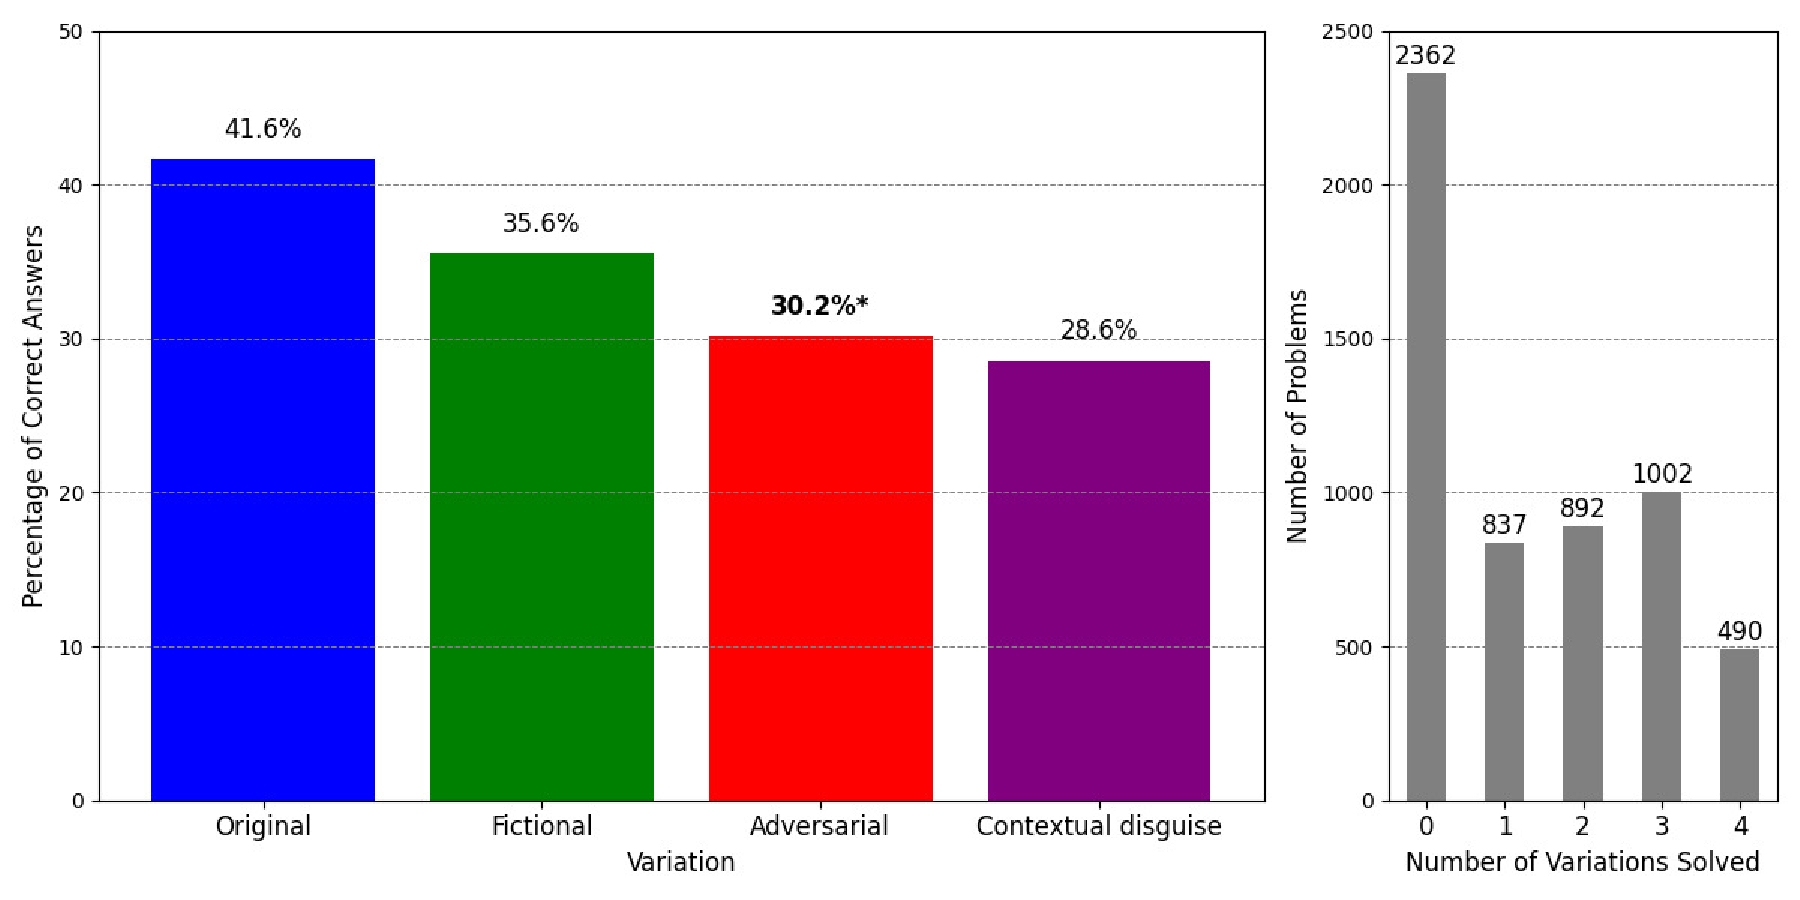
\includegraphics[width=0.9\textwidth]{synthetic_5583_avg.pdf}
    \caption{Ліворуч зображено частоту правильно розв'язаних варіацій до задач: оригінальна задача (блакитний), художня (зелений), суперечлива (червоний), прихована (фіолетовий). Праворуч зображено кількість правильно розв'язаних варіацій для кожної задачі. `*' вказує, що різниця у варіаціях була значуща ($p < .05$).}
    \label{fig:versions}
\end{figure}

\begin{figure}[ht]
    \centering
    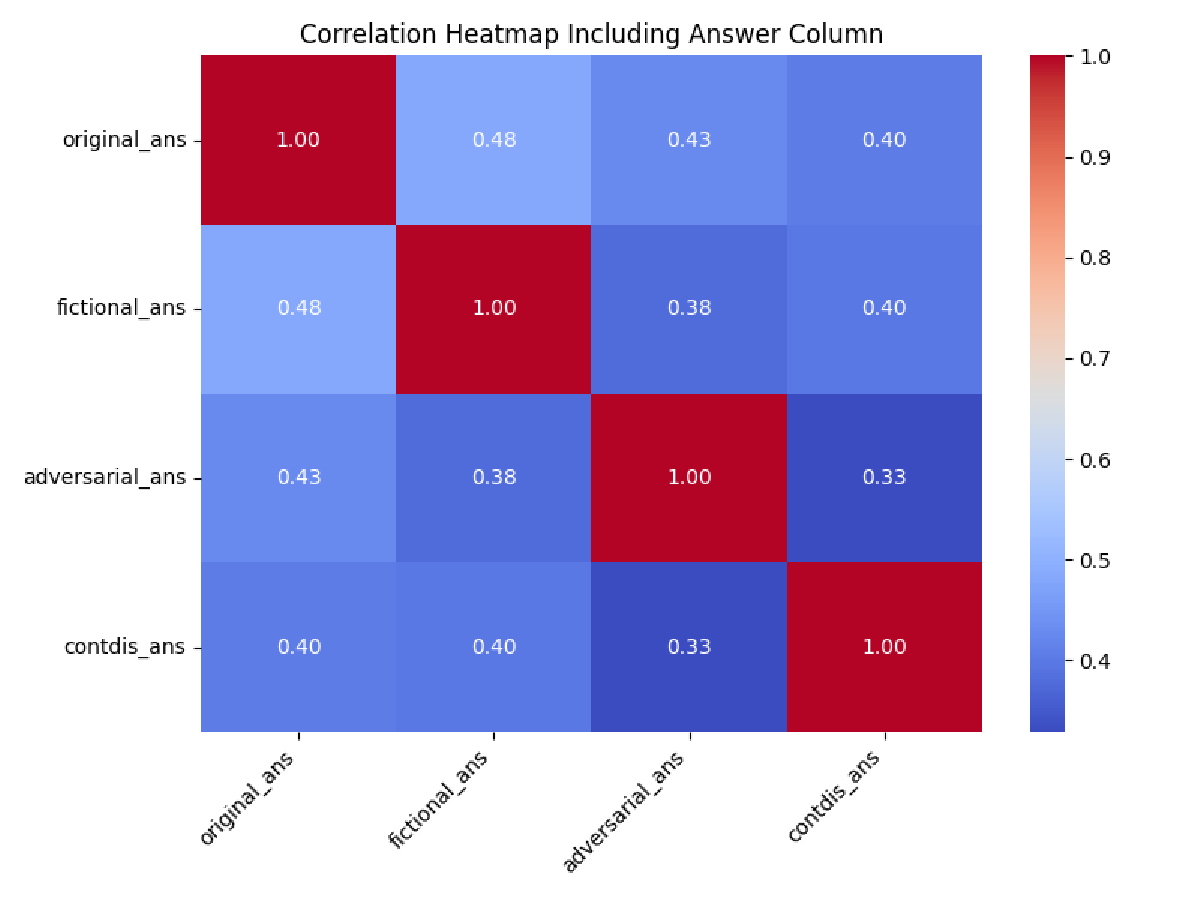
\includegraphics[width=0.9\textwidth]{synthetic_5583_corr.pdf}
    \caption{Коефіцієнт кореляції варіацій задач.}
    \label{fig:corr}
\end{figure}

Незважаючи на найбільшу середню довжину формулювання художньої варіації задачі ($len_{fictional}=651$ символів), дана варіація продемонструвала найкращі результати серед згенерованих синтетичний варіацій (35.6\%). Результати перевірки значущості показали, що порівняння між оригінальними розв'язками та розв'язками надлишкової варіації (\texttt{adversarial\_ans}) були значущими, у той час як порівняння з іншими варіаціями не виявили значних відмінностей. З наведених результатів також можна бачити, що у випадках, коли задача була розв'язана правильно, це було відбувалося у 3 з 4 варіацій задач (у 1002 випадках із 5583 протестованих задач), що також вказує на те, що принаймні рівно одна варіація у більшості випадків була не розв'язана моделлю.

Окремо слід зазначити, що під час проведення експериментально частини на 1000 тестових задачах, статистично значущою була різниця між оригінальними відповідями та відповідями надлишкової варіації (\texttt{contdis\_ans}) -- можлива ознака того, що збільшення набору даних призвело до покращення результатів оцінювання.

Для кореляційного аналізу було розглянуто результати різних варіацій, щоб побачити наскільки часто варіації однієї і тієї ж самої задачі розв'язувалися або не розв'язувалися моделлю правильно. На рисунку~\ref{fig:corr} видно слабку кореляцію між представленими варіаціями (між .33 і .48), що свідчить про те, що варіації не сильно пов'язані між собою. Це також свідчить про те, що процес генерації даних охоплює різноманітність, зберігаючи при цьому однакову результативність у кількості наданих правильних відповідей.

\subsection{Показник варіаційної узгодженості}

Для якості згенерованих моделей варіацій задач та їх впливу на точність розв'язань -- запропоновано нову метрику \textit{показник варіаційної узгодженості} (Variation Consistency Score). Ця метрика поєднує точність моделі та рівень кореляції між варіаціями задач, що дозволяє оцінити здатність моделей генерувати різноманітні, але точні із точки зору збереження сутності задачі тексти \cite{nikolaiev2025synth}.

Ця метрика поєднує в собі два ключові компоненти:

\begin{enumerate}
    \item \textbf{Частота правильних розв’язків (Solution rate)}: Відсоток правильно розв'язаних задач для заданої варіації моделлю.
    \item \textbf{Рівень кореляції варіацій (Correlation rate)}: Коефіцієнт кореляції між правильними відповідями та очікуваною відповіддю. Високий рівень кореляції свідчить про те, що варіації демонструють подібні результати та передають математичну основу задачі.
\end{enumerate}

Показник варіаційної узгодженості поєднує дані компоненти за допомогою середнього гармонійного значення (міри F1), забезпечуючи збалансовану оцінку, яка враховує точність роботи моделей та узгодженість варіації з оригінальною версією задачі. Даний показник обчислюється за наступною формулою:

\begin{equation}
\text{Variation Consistency Score} = \frac{2 \times (\text{Sol.rate} \times \text{Corr.rate})}{\text{Sol.rate} + \text{Corr.rate}}
\end{equation}

Показник варіаційної узгодженості акцентує увагу на ефективність роботи моделі: (i) оцінює наскільки модель є точною (відсоток правильно наданих відповідей по новій варіації задачі) і (ii) придатної до збереження математичної основи у новій варіації (висока кореляція між відповідями нової варіації та оригінальної) -- таким чином пропонуючи надійний показник для порівняння моделей у синтетичній генерації даних.

У таблиці \ref{tab:f1} наведено результати для варіацій задач, представлених у статті. Найвищу оцінку отримала художня варіація (.409) завдяки найвищій частоті правильності відповідей та високої кореляції з оригінальними даними.

\begin{figure}
    \centering
    \captionof{table}{Частота розв'язання (Sol.rate), коефіцієнт кореляції (Corr.rate) та показник узгодженості варіацій (Var.consist.)}
    \label{tab:f1}
    \begin{tabular}{|l|c|c|c|}
        \hline
        \textbf{Варіація} & \textbf{Sol.rate} & \textbf{Corr.rate} & \textbf{Var.consist.} \\
        \hline
        Художня & .356 & .482 & .409 \\
        Надлишкова & .302 & .428 & .354 \\
        Прихована & .286 & .404 & .335 \\
        \hline
    \end{tabular}
\end{figure}

%%%%%%%%%%%%%%%%%%%%%%%%%%%%%%%%%%%%%%%%%%%%%%%%%%%%%%%
\section{Аналіз результатів експерименту з участю експертів}

Наступний експеримент присвячено аналізу результатів експертів на наборі даних \emph{Combi-Puzzles}. Як згадувалося у підготовці експерименту у Розділі~\fullref{sec:human-experiment-set-up}, задля збереження репрезентативності експертів обиралися 5 учасників з найкращими результатами з кожної групи. Експерти певної групи отримували однаковий набір задач, проте працювали окремо один від одного.

Результати, представлені на Рисунку~\ref{fig:human_results}, свідчать, що експерти, середній вік яких становив 16 років, витратили в середньому 63 хвилини на розв’язання задач і у середньому отримали 70\% правильних розв'язків.

\begin{figure}
    \centering
    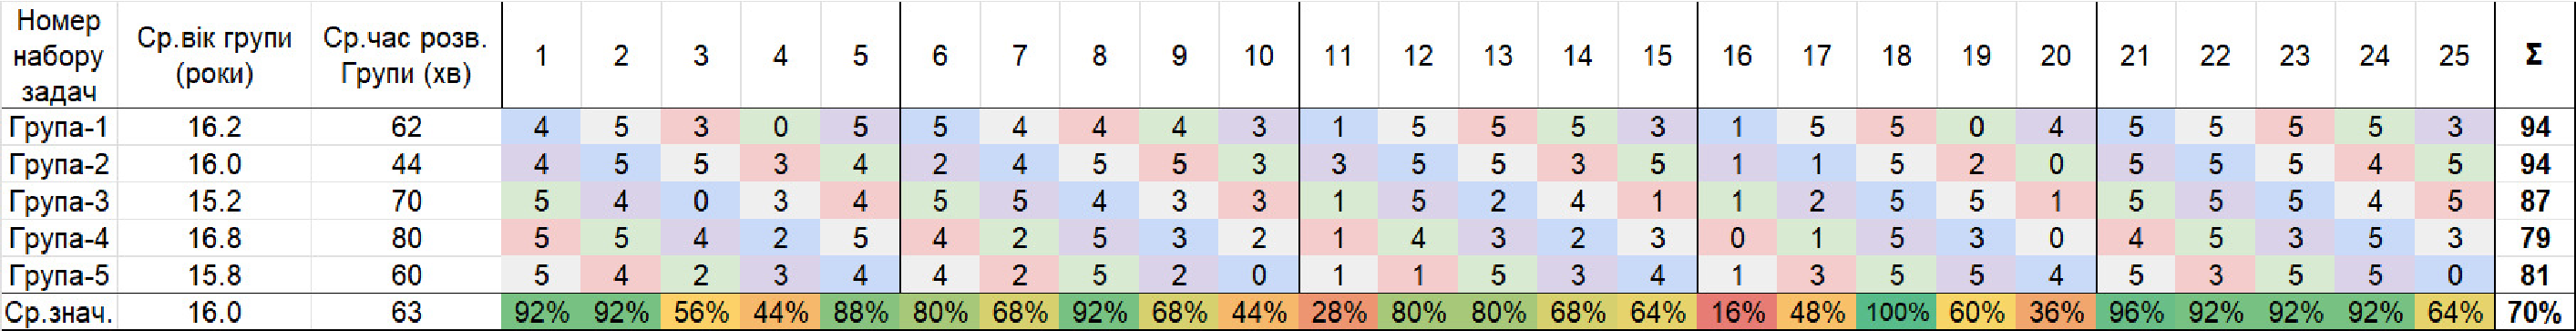
\includegraphics[width=1\textwidth]{data/human_results_top5.pdf}
    \caption{Результати 5 найкращих по кожній групі експертів на наборі задач Combi-Puzzles.}
    \label{fig:human_results}
\end{figure}

Загалом, усі експерти у своїх розв’язках забезпечили правильні рішення для кожної задачі щонайменше в одній з її варіацій. Проте, з Рисунку~\ref{fig:human_results} видно, що задачі 3, 4, 10, 11, 16, 17, 19 та 20 мають нижчі середні показники розв’язання (56\%, 44\%, 44\%, 28\%, 16\%, 48\%, 60\% та 36\% відповідно) порівняно з очікуваними 70\%.

У деяких випадках показник розв’язання був нижчим за очікуваний, що можна пояснити складністю певних задач. Наприклад, експерти надали лише кілька правильних розв’язків на задачі 11 та 16 (менше 30\% у всіх варіаціях), що може свідчити про їхню високу складність для розв’язання.

Для задач 4, 10, 16, 20 та 25 також спостерігалося, що жоден з експертів не зміг розв’язати задачу в одній або двох її варіаціях. Це може свідчити про те, що за певних змін умов задачі вони стають складними для розуміння навіть для експертів. Ці випадки будуть детальніше розглянуті у наступному підрозділі.

%%%%%%%%%%%%%%%%%%%%%%%%%%%%%%%%%%%%%%%%%%%%%%%%%%%%%%%
\section{Порівняння результатів роботи між моделями та експертами}

\begin{figure}
\centering
    \captionof{table}{Середні показники GPT-4 (без додаткової інструкції) та експертів за правильно розв’язаними задачами у різних умовах та загалом.}
    \begin{tabular}{|l|ccccc|c|}
        \hline
        Модель & Звич. & Матем. & Надлишк. & Парам. & Лінг. & Загал. \\
        \hline
        GPT-4 & .82 & .94 & .77 & .67 & .70 & .78 \\
        Експерти & .78 & .63 & .64 & .70 & .74 & .70 \\
        \hline
    \end{tabular}
    \label{tab:forms_human_v_model}
\end{figure}

У Таблиці~\ref{tab:forms_human_v_model} показано різницю в ефективності між експертами та ВММ за різними варіаціями задач і загалом. Із таблиці випливає, що найкраща модель (GPT-4) значно перевершує експертів у загальному показнику. Також спостерігається, що GPT-4 має високий результат у математичній формі задач (94\%), тоді як експерти досягли лише 63\%. Це може пояснюватися тим, що GPT-4 імовірно зустрічала подібні математичні тексти під час навчання.

Використання тесту Манна–Уїтні для порівняння середніх показників показало, що вплив математичної варіації є суттєвим ($p = .011 < .05$) порівняно з відсутністю математичної форми ($p = .281 > .05$). Для надлишкової варіації GPT-4 отримала вищий показник (77\%) порівняно з експертами (64\%), проте різниця не виявилася статистично значущою ($p=.185$). Надлишкова варіація створена додаванням нерелевантної інформації до звичайної постановки задачі, що, ймовірно, спричиняє більшу плутанину для експертів.

У випадку лінгвістичного заплутування різниця між моделями та експертами є набагато меншою (70\% для GPT-4 проти 74\% в експертів) і навіть трохи краща для останніх. Проте ця різниця не визнається статистично значущою ($p=.714$). Одна з гіпотез полягає в тому, що ефективність GPT-4 у лінгвістично заплутаній варіації знижується через більшу кількість тексту, що ускладнює виокремлення релевантної інформації.

Для параметризованої форми ефективність GPT-4 порівняно з експертами майже однакова (67\% проти 70\%), що може свідчити про недостатню точність моделі під час обчислень із більшим обсягом арифметики. У деяких випадках було відзначено, що попри правильні кроки обґрунтування GPT-4 могла генерувати неправильні ланцюги виразів, що призводило до хибних результатів.

З Таблиці~\ref{tab:forms_diff} видно, що результативність GPT-4 є чутливою до відмінностей у формулюваннях задач, які було задано п’ятьма формами у нашому наборі даних. Зокрема, було виявлено, що GPT-4 значно краще розв’язує комбінаторні задачі, подані в математичній формі (94\%), порівняно з надлишковими, лінгвістично заплутаними та параметризованими варіаціями (77\%, 70\% та 67\% відповідно). Це свідчить про певну нездатність моделі до узагальнення у міркуванні без додаткових етапів навчання моделей. Утім, дані висновки отримані на дослідження роботи моделей з набором даних Combi-Puzzles, які підтвердження у відповідному дослідженні.

Водночас, різниця у частоті надання правильних розв'язків експертами серед різних варіацій не є статистично значною. Це вказує на те, що здатність експертів до розв’язання комбінаторних задач не є залежною до модифікацій текстів задач.

На деяких варіаціях модель GPT-4 значно перевершує експертів, особливо у задачах із чітким формулюванням (математична варіація) і без додаткових лінгвістично-стилістичних маніпуляцій. Проте експерти виявляються більш гнучкими у розв’язанні задач з нестандартними умовами та можуть краще адаптуватися до модифікацій у формулюванні задач \cite{nikolaiev2024can}.

\section{Детальний аналіз окремих випадків задач}

\begin{figure}
    \centering
    \begin{subfigure}{\linewidth}
        \centering
        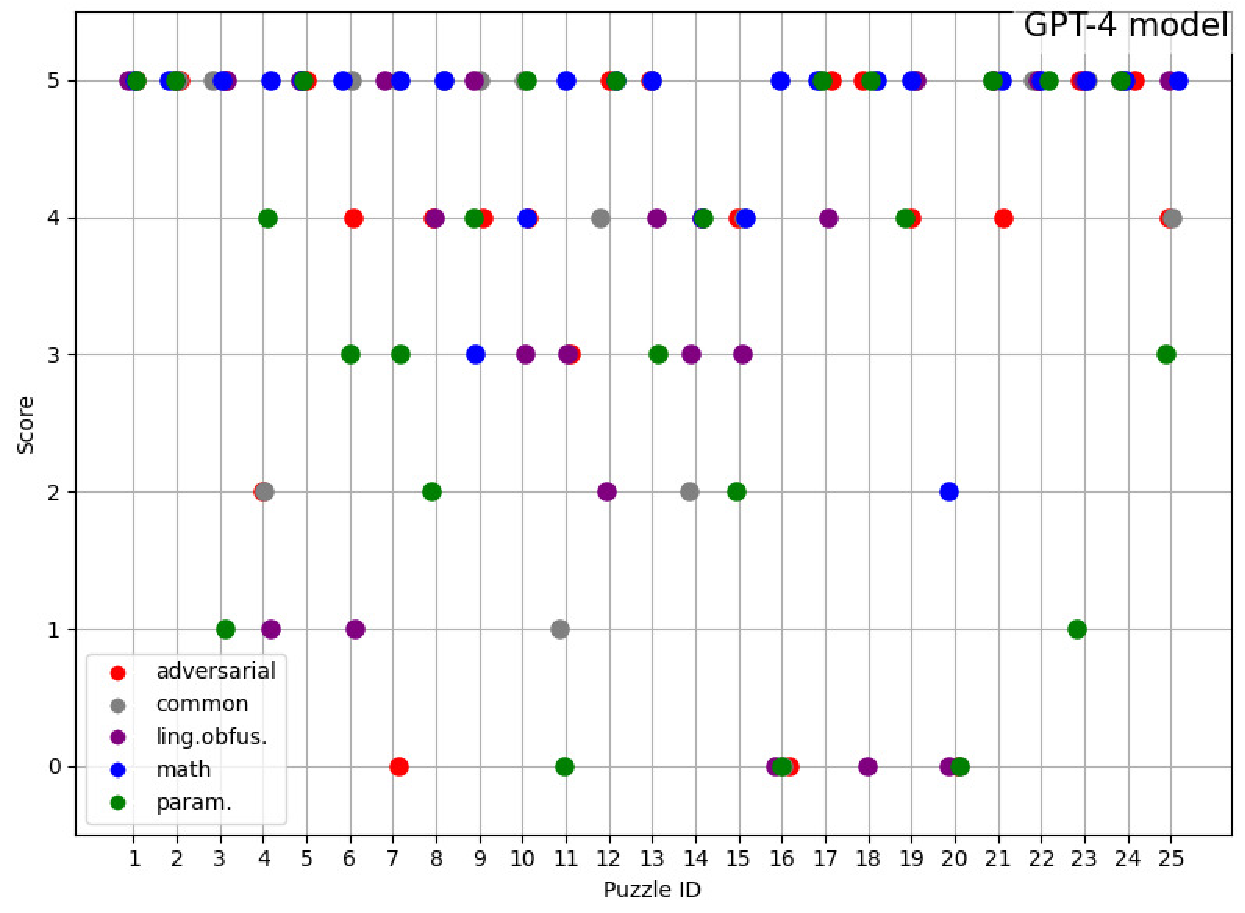
\includegraphics[width=0.75\linewidth]{data/Image-GPT-4.pdf}
        \caption{GPT-4}
        \label{fig:subimage_gpt4}
    \end{subfigure}
    \begin{subfigure}{\linewidth}
        \centering
        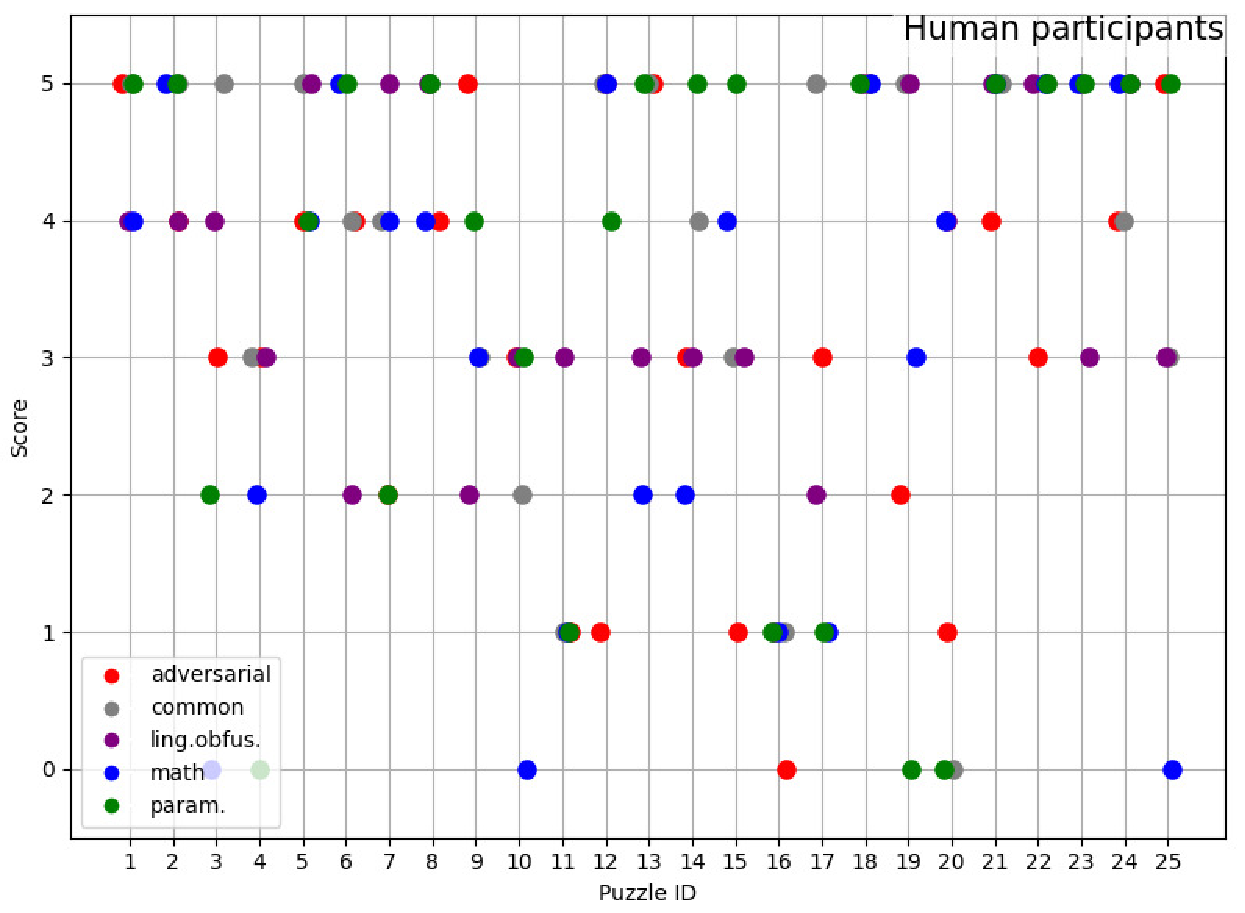
\includegraphics[width=0.75\linewidth]{data/Image-Humans.pdf}
        \caption{Експерти}
        \label{fig:subimage_humans}
    \end{subfigure}
    \caption{Індивідуальні бали за задачі та відсоток правильних розв’язків, представлені для GPT-4 та експертів.}
    \label{fig:humans_v_models_problems}
\end{figure}

Аналіз окремих задач надав можливість з’ясувати, які варіації задач були найскладнішими для експертів та ВММ. На Рисунку~\ref{fig:humans_v_models_problems} зображено кількість правильних розв’язків, наданих GPT-4 та експертами по кожній варіації задач у наборі \emph{Combi-Puzzles}. По осі X зазначено номер задачі, а по осі Y -- кількість правильних розв’язків. Результати тестування моделі GPT-4 формувалися на основі 5 запитів (кожен запит виконувався у окремій сесії), а результати тестування експертів -- з 5 учасників з найкращим результатом серед кожної групи.

З Рисунку~\ref{fig:humans_v_models_problems} видно, що кількість правильних розв’язків наданих експертами варіюється більше ніж кількість розв’язків від GPT-4. Модель має більш поляризовану тенденцію: якщо GPT-4 здатна розв’язати відповідну задачу у запропонованій варіації, вона зберігає цей результат на решті запитів. Натомість здатність експертів розв’язати задачі у різних варіаціях залежить від індивідуальних особливостей кожного учасника та їхнього досвіду у комбінаториці.

Також помітно, що в деяких випадках жоден з запитів моделі GPT-4 та експерти не надали жодного правильного розв’язку для окремих задач. Зокрема, задачі p4/param, p10/math та p25/math були розв’язані GPT-4 у 4, 5 та 5 випадках відповідно, тоді як експерти не дали жодного правильного розв’язку. Аналогічно задачі p18/ling.obfus та p20/ling.obfus були розв’язані експертами у 5 та 4 випадках відповідно, тоді як GPT-4 не надала жодного правильного розв’язку. Повні формулювання цих задач наведено у таблиці~\ref{tab:problems-poorly-solved}. Кожну задачу та її варіацію у таблиці задано ідентифікатором у вигляді ProblemID/variation. У відповідних стовпчиках таблиці зазначено кількість разів, коли задачу було правильно розв'язано (1) моделлю GPT-4 та (2) експертами. Тексти задач наведені українською мовою, якою проводилося експериментальна частина з людьми. Моделі під час експериментування працювали з англійськими текстами задач. Мови були обрані відповідно до того, на яких моделі мали більше попереднього тренування, а учасники -- математичного шкільного досвіду.

% \renewcommand{\arraystretch}{0.8} % change the interval between lines
\begin{figure}[!h]
    \centering
    \small
    \captionof{table}{Деякі приклади задач з найгіршими результатами розв'язання серед моделі GPT-4 (а) та експертів (б).}
    \label{tab:problems-poorly-solved}
    \begin{tabular}{|p{14cm}|c|c|}
        \hline
        \textbf{ID задачі та Умова} & \textbf{а} & \textbf{б} \\
        \hline
        \textbf{p4/param:} У кінотеатрі черга на фільм. Квиток коштує 5 фунтів. 5 людей мають банкноту у 10 фунтів кожна, і ще 5 людей мають банкноту у 5 фунтів кожна. На початку касир немає решти. Скільки існує різних способів формування черги, щоб кожен міг купити квиток? & 4 & 0 \\
        \hline
        \textbf{p10/math:} У скрині є 3 кулі, які пронумеровані від 1 до 3. Ви дістаєте кулі 9 разів одну за одною, кожного разу повертаючи кулю назад до скрині. Скільки різних можливих наборів куль ви можете отримати? & 5 & 0 \\
        \hline
        \textbf{p18/ling.obfus:} Лицар, який живе у місті Ґрінфілдс, планує брати участь на щорічних лицарських змаганнях. По-перше, він повинен доїхати до містечка Понівіль, де отримає свого благородного скакуна. Є 3 дороги між Ґрінфілдсом і Понівілем. У нього є вибір з 7 коней у Понівилі. Після цього він повинен поїхати у місто Садделфорд та обрати новий блискучий та комфортний садунок. Є 5 доріг між Понівілем і Садделфордом. Скільки існує шляхів, щоб подорожувати з Ґрінфілдса до Садделфорда через Понівіль? & 0 & 5 \\
        \hline
        \textbf{p20/ling.obfus:} Ви керуєте двома островами та церемоніальним човном, і ваша робота полягає у тому, щоб зробити кілька підготувань до важливого фестивалю. На кожному острові знаходять найвище дерево, яке потім вирізають у тотем, щоб розмістити на пляжі. Як тільки зрубають одне з двох дерев, на материк надсилається телеграма разом з датою та часом. Коли один з двох тотемів встановлено на пляжі, надсилається інша телеграма. Також вам потрібно переконатися, що церемоніальний човен буде прикрашено. Коли й ця робота буде завершена, надсилається ще одна телеграма. У вас є працівники на кожному острові та човні. Ви не знаєте, скільки часу займає кожна робота. Наприкінці підготувань ви дивитесь на порядок отриманих телеграм. Скільки існує різних послідовностей? & 0 & 4 \\
        \hline
        \textbf{p25/math:} У скрині знаходиться 25 куль білого кольору, які пронумеровані від 1 до 25, та 25 куль чорного кольору, які пронумеровані від 1 до 25. Ви дістаєте по одній 25 куль, не повертаючи їх назад до скрині. Щоразу коли ви дістаєте кулю з номером N певного кольору, куля з таким самим номером іншого кольору зникає зі скрині. Скільки різних послідовностей куль існує, які містять максимум 3 чорних кулі? & 5 & 0 \\
        \hline
    \end{tabular}
\end{figure}

У задачі p25/math комбінаторний розв’язок містить окремі підзадачі з нулем, однією та кількома чорними кулями, після чого застосовується правило суми: \(C(25, 0) + C(25, 1) + C(25, 2) + C(25, 3) = \sum_{i=0}^{3} C(25, i)\). Аналіз розв’язків GPT-4 свідчить, що модель правильно поділила задачу на підзадачі, розв’язала їх і підсумувала результати. Дана задача є однією з найскладніших у наборі даних, її математичну варіацію не розв’язав жоден з експертів.

Також GPT-4 продемонструвала кращий результат у задачі p10/math порівняно з експертами. Експерти не врахували, що шукається \textit{кількість різних наборів} куль, і надали розв’язок \(3^9\). Натомість GPT-4 правильно розпізнала умову й обрала відповідну комбінаторну формулу: \(C(11, 2) = 55\).

В окремих випадках модель GPT-4 виявляла здатність ідентифікувати математичні концепції у задачах та застосовувати їх для розв’язання більших складних випадків параметризованої варіації задач. Наприклад, у задачі p4/param GPT-4 розпізнала послідовність чисел Каталана і відразу використала формулу \(C_n = \frac{(2n)!}{(n + 1)!n!}\), що дозволило отримати правильний розв'язок.

Водночас GPT-4 мала певні труднощі з розв’язанням варіацій лінгвістичного заплутування, які вважаються одними з найпростіших у наборі даних: задачі p18/ling.obfus та p20/ling.obfus були успішно розв’язані експертами, тоді як GPT-4 не надала жодного правильного розв’язку. Це свідчить про те, що додавання нерелевантної інформації або зміна стилю викладу задачі ускладнюють для моделі відокремлення суттєвої інформації задачі.

Прикладом додаткових умов є задача: ``Визначте кількість різних способів, якими тура може переміститися з початкової до кінцевої позиції на шаховій дошці 3×3, \textit{не проходячи через середню клітинку.}''. Усі три конфігурації моделі LLaMA 3.1 (з урахуванням 8, 70 та 405 млрд. параметрів) успішно розв’язали початкову версію задачі, надавши правильний розв’язок. З  рис.~\ref{fig:prob_constraints} можна бачити, що у випадку з додатковим обмеженням про заборону використання середньої клітинки дошки, модель неправильно порахувала кількість можливих шляхів. Натомість експерти не зазнали подібних труднощів, правильно зазначивши, що кількість правильних шляхів дорівнює 2.

\begin{figure}[h]
    \centering
    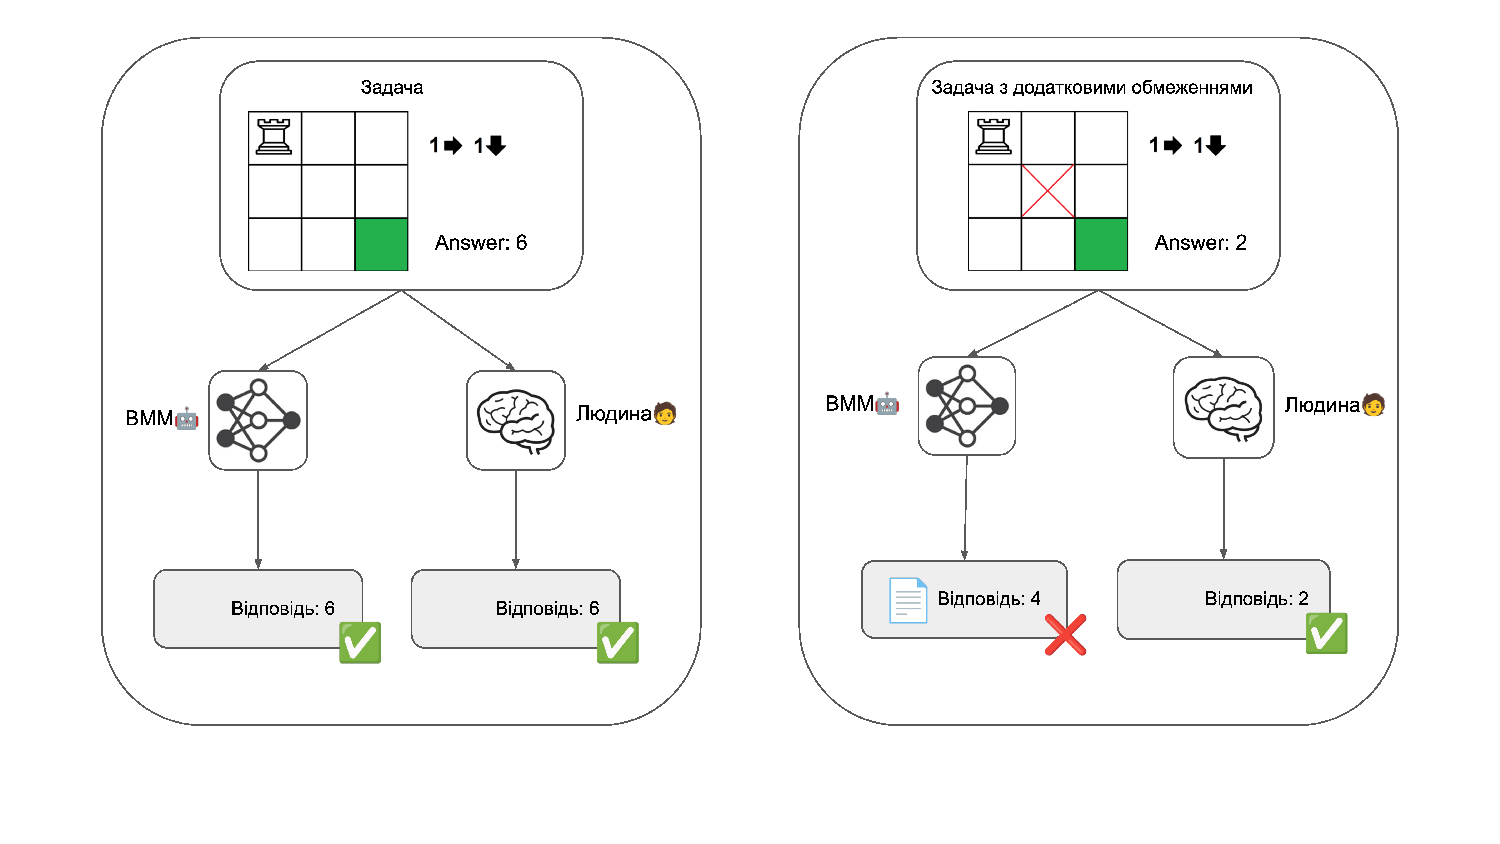
\includegraphics[width=1\textwidth]{prob_constraints.pdf}
    \caption{LLaMA 3.1 і експерти, що розв’язують комбінаторну задачу у двох умовах: звичайну версію та з додатковими обмеженнями.}
    \label{fig:prob_constraints}
\end{figure}

Таким чином, виявлено що моделі не завжди здатні розв'язувати задачі через неправильне розуміння умов або неможливість врахувати усі можливі варіанти відповіді. Наприклад, мовні моделі закономірно пропускають ключові деталі або не враховувати додаткові обмеження, що свідчить про потребу подальшого вдосконалення самоаналізу на необхідності внутрішнього міркування моделей.

\section{Висновки та подальші дослідження}

\paragraph{Вплив математичних роздiлiв на ефективність моделей при розв'язанні задач.}
Дослідження демонструє застосування передових мовних моделей для оцінки ефективності розв’язання задач у різних математичних розділах. Під час роботи з набором даних NuminaMath-TIR було виявлено значні відмінності у ефективності роботи моделей у генерації розв'язків між виділеними математичними розділами: алгебра, геометрія, теорія чисел та комбінаторика. Результати підтверджують статистично значущу залежність між математичними розділом та частотою правильних розв’язків. Найбільш складною темою виявилася комбінаторика, на якій протестовані моделі продемонстрували найнижчі результати.

Проведений аналіз засвідчує послідовні закономірності поведінки протестованих моделей: розділ алгебри зазвичай дає найвищі результати для всіх моделей, що свідчить про високу здатність працювати з формальними текстами. Водночас комбінаторика стабільно виявляється найскладнішою для пошуку правильних розв’язань у більшості випадків. Врахування особливостей походження математичних задач є важливим для подальшого покращення роботи моделей при розв'язанні математичних задач. Зокрема, важливим є підготовка та класифікація навчальних наборів даних орієнтованих для виправлення в ефективності моделей за різноманітними розділами.

Хоча усі відмінності в ефективності моделей між розділами були значущими, спостерігалося, що деякі моделі, зокрема GPT-4o-mini і Llama-3.1-8B-Instruct, виявляють більшу чутливість до відповідних розділів задач ($\chi^2_{\text{}}>180$). Для моделей Mathstral-7B та Qwen2.5-Math-7B характерні більш стабільні показники ефективності в розділах задач ($\chi^2_{\text{}}<150$). Це підкреслює важливість використання таких технік, як інтегроване розуміння з інструментами ToRA, задля отримання більш стабільних результатів моделей по різних математичних розділах задач. Про це також свідчать результати ВММ Qwen2.5-Math-7B, яка згідно опису має інтегрований ToRA, але незважаючи на відносно невеликий розмір моделі, показала вищу загальну ефективність у всіх розділах задач.

Ці результати наголошують на важливості врахування специфіки розділів різноманітних математичних задач для подальшого дослідження моделей у галузі обробки математичних даних. Це може сприяти створенню адаптивних систем навчання, здатних ефективно сприймати тонкощі різних математичних розділів.

\paragraph{Висновки дослідження з набором даних Combi-Puzzles}
Було запроваджено набір даних \emph{Combi-Puzzles} для оцінки здатності ВММ до міркування у комбінаторних задачах та методологію для створення наборів даних для цього завдання. За підсумками результатів експериментів GPT-4 продемонструвала найбільш високу роботу з математичними комбінаторними задачами серед протестованих ВММ. Зокрема, було встановлено, що модель у середньому повертає більшість кількість правильних розв'язків у порівнянні з учасниками з олімпіадним досвідом.

Результати свідчать про те, що здатність GPT-4 до міркувань вища, коли комбінаторні задачі представлені у формально-математичному стилі (математична варіація, 94\%). Однак також було установлено, що у наведеному наборі даних ефективність GPT-4 значно погіршується, коли у текстах задачі вводиться зайва інформація (надлишкова варіація, 77\%), коли умова задачі представлена у незнайомому наративному стилі (лінгвістичне заплутування, 70\%), а також при зміни параметрів задачі (параметризована варіація, 67\%). Незважаючи на гірші середні показники, учасники у дослідженні мали різні  надання правильних точності на досліджуваних варіаціях задач, не було виявлено залежностей між частотою надання правильних розв'язків та варіаціями задач.

\paragraph{Вдосконалені методів генерації синтетичних комбінаторних задач}
У роботі було проведено дослідження використання нейромережевих методів відбору та генерації синтетичних варіацій комбінаторних задач із залученням сучасної великої мовної моделі GPT-4o-mini. За допомогою запропонованого методу було відібрано дані та згенеровано синтетичні варіації, зберігаючи основний зміст математичних задач. Це дозволило оцінити здатність моделей до узагальнення міркування та слідування заданим інструкціям. Знайти приклади згенерованих задач можна у Додатку~\fullref{sec:problems-synthetic}.

Статистичний аналіз за допомогою тестів на перестановку показав, що модель не виявляє суттєвих відмінностей у розв'язанні введених варіацій задач порівняно з оригінальною, за винятком \emph{прихованої варіації}, яка отримала найнижчі оцінки. Водночас кореляційний аналіз варіацій, згенерованих нейромережевими методами, показав, що задачі мають низький рівень взаємозв'язку між собою. Знижений ризик повторюваності означає, що кожна варіація робить унікальний внесок у процес генерації текстів.

Окрім цього, для оцінювання здатності моделі до узагальнення було введено нову метрику -- \emph{Показник варіаційної узгодженості}, який поєднує частоту правильно наданих розв'язків задач та їхньою відповідністю оригінальним текстам. За результатами експериментування, незважаючи на найбільший розмір оброблених текстів, \emph{художня варіація} зберегла найвищу оцінку якості. Дані результати свідчать про те, що модель здатна генерувати унікальні та точні математичні дані, зберігаючи їхню математичну основу.

У майбутніх дослідженнях підкреслюється важливість підвищення адаптивності моделей шляхом вивчення вдосконалених методів навчання, які покращують обробку різноманітних текстових маніпуляцій. Це може бути досягнуто шляхом впровадження стратегій тренування моделей та нейро-символічних систем, а також використання різноманітних навчальних наборів даних. Зусилля в цьому напрямку можуть призвести до покращення загальної здатності моделей до узагальнення та підвищення їхньої стійкості в задачах математичного міркування.

\paragraph{Обмеження ВММ та напрямки подальших розробок}
Попри значущість отриманих результатів, дослідження має певні обмеження. Було продемонстровано, що мовні моделі виявляють високу чутливість до змін у формулюванні задач, що знижує точність розв'язань при введенні зайвої інформації або лінгвістичних модифікацій.

Складність комбінаторних задач та їх математичний підтекст іноді перевищують здатності моделей до адекватного міркування, що потребує інтеграції формальних методів, яку можна досягнути за рахунок розробки автоматизованих систем перевірки й формалізації синтетичних даних для забезпечення більш стабільної якості генерованих результатів.

Подальші дослідження можуть бути зосереджені на розробці модифікованих архітектур великих мовних моделей, стійкіших до стилістичних варіацій та надлишкової інформації. Такі архітектури мають передбачати інтеграцію формальних методів міркування й символьних обчислень з ВММ для підвищення точності та послідовності математичних розв'язань.

Іншим напрямком для поліпшення існуючих методів за рахунок отриманих результатів є розширенні підходів генерації синтетичних даних, з метою охоплення ширшого спектру математичних задач різних математичних розділів.

Не можна також забувати про важливість етичних аспектів використання штучного інтелекту в освіті та наукових дослідженнях, які сприяють подальшому вдосконаленню автоматизованих освітніх систем.

\paragraph{Практичне значення та перспективи використання отриманих результатів}
Практичне значення проведеного дослідження полягає в наступному:
\begin{itemize}
    \item Розроблені методи синтезу даних та генерації комбінаторних задач можуть бути використані для покращення адаптивних освітніх систем, що підтримують автоматизований процес навчання та оцінки учнів.
    \item Запропонована методологія формалізації математичних текстів дозволяє оптимізувати процес переведення задач з природної мови у формальні математичні вирази, що має важливе значення для розвитку автоматизованих систем доведень.
    \item Використання нової метрики варіаційної узгодженості дає можливість здійснювати більш глибокий аналіз якості генерованих даних, що може стати основою для подальших досліджень та комерційних застосувань у сфері штучного інтелекту.
    \item Результати експериментального дослідження сприяють побудові міцного містка між можливостями ВММ та практичними потребами математичної освіти та наукових розробок.
\end{itemize}

Таким чином, було проведено комплексний аналіз якості науково-методичного апарату, що підтверджує доцільність впровадження запропонованих кроків з метою покращення алгоритмів генерації розв’язань і синтезу даних математичних комбінаторних задач. Дані результати мають важливе значення для подальших досліджень за напрямком розвитку моделей у математичних задачах і практичного застосування мовний моделей у освітньо-практичних цілях.

\chapter*{Висновки}

У даній дисертаційній роботі проведено комплексне дослідження можливостей великих мовних моделей для синтезу даних, генерації математичних комбінаторних задач та автоматичної формалізації математичних текстів. Результати роботи підтверджують актуальність і доцільність застосування сучасних нейромережевих підходів для вирішення завдань математичного міркування. Основні наукові досягнення роботи можна підсумувати наступним чином:
\begin{itemize}
    \item Проведено огляд стану сучасних методів для обробки природної мови та моделей штучного інтелекту для роботи з математичними задачами, зокрема архітектур моделей для генерації текстів, методів машинного навчання, інженерії запитів при роботі з мовними моделями, задіяння додаткових інструментів для символьної обробки даних, існуючих наборів даних та метрик оцінювання. Виділено особливості різних типів математичних задач та проведено повіряння ефективності моделей у генерації розв'язків за допомогою версій мовних моделей GPT-4, Qwen, LLaMA та Mistral.
    \item Розроблено набір даних \emph{Combi-Puzzles}, який включає набір з комбінаторних задач з систематичною модифікацією умов за рахунок керування наступними параметрами та особливостями задач: конфігурація параметрів задачі, додавання зайвої інформації, зміна лінгвістично-стилістичної формату тексту умов задач.
    \item Проведено експериментальне порівняння ефективності моделей до розв'язання математичних комбінаторних задач на синтезованих даних та оцінено більш ніж 36 тис. із залученням сучасних ВММ із різними архітектурами та інтегрованими методами для проведення математичного міркування, зокрема з версіями моделей GPT-4, LLaMA, Mixtral у кількох розмірах та специфікаціях.
    \item Проведено експериментальну частину з залученням людей-експертів, які мають олімпіадний математичний досвід. Результати експертів додані як метрика для оцінювання ефективності роботи ВММ. Порівняльний аналіз показав, що мовні моделі здатні демонструвати високу точність у розв'язанні задач заданих на вхід у формальному вигляді, водночас з цим їхня ефективність суттєво знижується за наявності додаткового інформаційного шуму та стилістичних змін текстів задач.
    \item Запропоновано новий метод для генерації синтетичних варіацій математичних комбінаторних задач через систематичну маніпуляцію текстів за рахунок контролю параметрів задач. Для оцінювання якості згенерованих даних запроваджено нову метрику \emph{Показник варіаційної узгодженості}, яка дозволяє оцінити якість генерованих синтетичних даних через аналіз частоти правильних розв'язків і коефіцієнтів кореляції між варіаціями задач. Цей підхід сприяє розширенню навчальних корпусів і підвищенню варіативності даних.
\end{itemize}

Отримані результати підтверджують виконання поставлених завдань і досягнення загальної мети дослідження щодо синтезу даних та генерації математичних комбінаторних задач за допомогою великих мовних моделей.

Проведене дослідження демонструє високий потенціал великих мовних моделей у генерації математичних текстів і вдосконаленні систем автоматизованого пошуку доведень. Розроблені методи не лише підвищують ефективність методів генерації синтетичних математичних задач, а й відкривають нові можливості для інтеграції нейромережевих підходів із формальними методами. Отримані результати становлять важливий внесок у сучасний напрям дослідження штучного інтелекту, який спрямований на розвиток методів обробки і генерації даних, а також є важливим для подальшої інтеграції відповідних систем у навчальні середовища, тести та платформи для дистанційного навчання, що сприяє її використанню у реальних освітніх процесах.

Таким чином, дисертаційна робота підтверджує досягнення поставленої мети та сприяє подоланню існуючих викликів у цій галузі. Отримані результати закладають основу для подальших наукових розробок у сфері обробки природної мови та штучного інтелекту, спрямованих на ефективну роботу з математичними даними.


% Література
\bibliography{sections/References}
\newpage

% Додатки
\appendix

\chapter{Список публікацій здобувача за темою дисертації}
\vspace*{-1\baselineskip}
\textit{\textbf{Наукові праці, в яких опубліковані основні наукові результати дисертації:}}
\medskip

\begin{enumerate}
    \item Ніколаєв, Андрій Д. та Анісімов, Анатолій В. \textit{Нейромережеві методи відбору та генерації синтетичних варіацій комбінаторних задач}. Кібернетика та системний аналіз. 2025, том 61, випуск 3, с.22-32. DOI: \url{https://doi.org/10.34229/KCA2522-9664.25.3.3}.
    \item Ніколаєв, Андрій. \textit{Нейромережеві методи формалізації математичних текстів}. Herald of Khmelnytskyi National University. Technical sciences, 345.6(2), 2024, с. 50—55. DOI: \url{https://doi.org/10.31891/2307-5732-2024-345-6-6}.
    \item Nikolaiev, Andrii D. та Derevianchenko, Oleksandr V. \textit{Comparison of Problem-solving Performance Across Mathematical Domains With Large Language Models}. Shtuchnyy intelekt, 2024, с. 96—104. \url{https://doi.org/10.15407/jai2024.04.096}.
    \item Власенко, О.В., Картавих, В.Ю., Ніколаєв, А.Д., Горбенко, В.І. \textit{Методика визначення опорної матриці моніторингу домена управління інформаційної мережі спеціального призначення}. Системи і технології зв’язку, інформатизації та кібербезпеки. Збірник наукових праць ВІТІ, випуск 4, 2019, с. 46—57.
\end{enumerate}

\medskip
\textit{\textbf{Наукові праці, які засвідчують апробацію матеріалів дисертації:}}
\medskip

\begin{enumerate}
    \item \textit{Introducing constraints in combinatorial problems: A case study with LLaMA 3.1}. -- 11th International Scientific Conference "Information Technology and Implementation (IT\&I-2024 Satellite)". Taras Shevchenko National University of Kyiv, 2024.
    \item \textit{AI in education: Application of LLMs for learning mathematics.} -- Ukrainian Cambridge: New Research by Displaced Scholars from Ukraine. University of Cambridge, 2023.
    \item Nikolaiev, Andrii D. and Anisimov, Anatoliy V. \textit{Mathematical word problem solution evaluation via data preprocessing approach}. 8th International Scientific Conference "Information Technology and Implementation (IT\&I-2021)", Vol. 3132, 2022, p. 94—103. \url{https://ceur-ws.org/Vol-3132/Paper_9.pdf} %\url{https://www.scopus.com/inward/record.uri?eid=2-s2.0-85129578190&partnerID=40&md5=63f41d66fe66b0b9088484ef474dcd4e}
    \item \textit{Implementation of Artificial Intelligence Module for Educational Purposes}. -- 7th International Scientific Conference "Information Technology and Interactions (IT\&I-2020 Satellite)". Taras Shevchenko National University of Kyiv, 2020.
\end{enumerate}

\medskip
\textit{\textbf{Наукові праці, які додатково відображають наукові результати дисертації:}}
\medskip
\begin{enumerate}
    \item Nikolaiev, Andrii, Stathopoulos, Yiannos та Teufel, Simone. \textit{Can language models rival mathematics students? Evaluating mathematical reasoning through textual manipulation and human experiments}. arXiv preprint, 2024. \url{https://arxiv.org/abs/2412.11908}.
\end{enumerate}

\chapter{Опис та доступи до протестованих моделей}
\label{sec:models-tested-links}
\vspace*{-1\baselineskip}
Детальні описи відкритих моделей (квантованих версій) та моделей від OpenAI доступні за наступними посиланнями:
\begin{enumerate}
    \item \textbf{LLaMA-2-7B-Chat}:\\
    \url{https://huggingface.co/TheBloke/Llama-2-7B-Chat-GGUF}.
    \item \textbf{LLaMA-2-13B-Chat}:\\
    \url{https://huggingface.co/TheBloke/Llama-2-13B-chat-GGUF}.
    \item \textbf{LLaMA-2-70B-Chat}:\\
    \url{https://huggingface.co/TheBloke/Llama-2-70B-Chat-GGUF}.
    \item \textbf{LLaMA-3.1-8B-Instruct}: \\
    \url{https://huggingface.co/QuantFactory/Meta-Llama-3.1-8B-Instruct-GGUF}.
    \item \textbf{LLaMA-3.1-70B-Instruct}:\\
    \url{https://huggingface.co/bartowski/Meta-Llama-3.1-70B-Instruct-GGUF}.
    \item \textbf{LLaMA-3.1-405B-Instruct}: (доступна через API)\\
    \url{https://build.nvidia.com/meta/llama-3_1-405b-instruct/modelcard}. 

    \item \textbf{Mixtral-8x7B}:\\
    \url{https://huggingface.co/TheBloke/Mixtral-8x7B-v0.1-GGUF}.
    \item \textbf{Mixtral-8x7B-Instruct}:\\
    \url{https://huggingface.co/TheBloke/Mixtral-8x7B-Instruct-v0.1-GGUF}.
    \item \textbf{Mathstral-7B}: \\
    \url{https://huggingface.co/QuantFactory/mathstral-7B-v0.1-GGUF}.

    \item \textbf{Qwen2-7B-Instruct}: \\
    \url{https://huggingface.co/QuantFactory/Qwen2-7B-Instruct-GGUF}.
    \item \textbf{Qwen2-Math-7B}: \\
    \url{https://huggingface.co/QuantFactory/Qwen2-Math-7B-GGUF}.
    \item \textbf{Qwen2.5-Math-7B}: \\
    \url{https://huggingface.co/QuantFactory/Qwen2.5-Math-7B-GGUF}.
    
    \item \textbf{GPT-4-Turbo}: (доступна через API)\\ 
    \url{https://platform.openai.com/docs/models/#gpt-4-turbo-and-gpt-4}.
    \item \textbf{GPT-4o-mini}: (доступна через API)\\
    \url{https://platform.openai.com/docs/models/gpt-4o-mini#gpt-4o-mini}.
\end{enumerate}

\chapter{Повні результати учасників експерименту}
\label{sec:humans-results-detailed}
\vspace*{-1\baselineskip}

На рис.~\ref{fig:human_results_detailed} можна бачити детальні результати роботи учасників у розв'язанні задач набору Combi-Puzzles.

Результати включають усіх 35 учасників, результати учасників ранжовані від найкращого до найгіршого у кожній з груп. Для формування загальних результатів, обиралися 5 ``експертів'' у кожній з груп (25 учасників разом) згідно постановки експерименту.

``0'' свідчить про те, що відповідь учасника була неправильною, ``1'' -- правильною, мінус -- учасник не передав відповідь на задачу (еквівалентно ``0'').

\begin{figure}
    \centering
    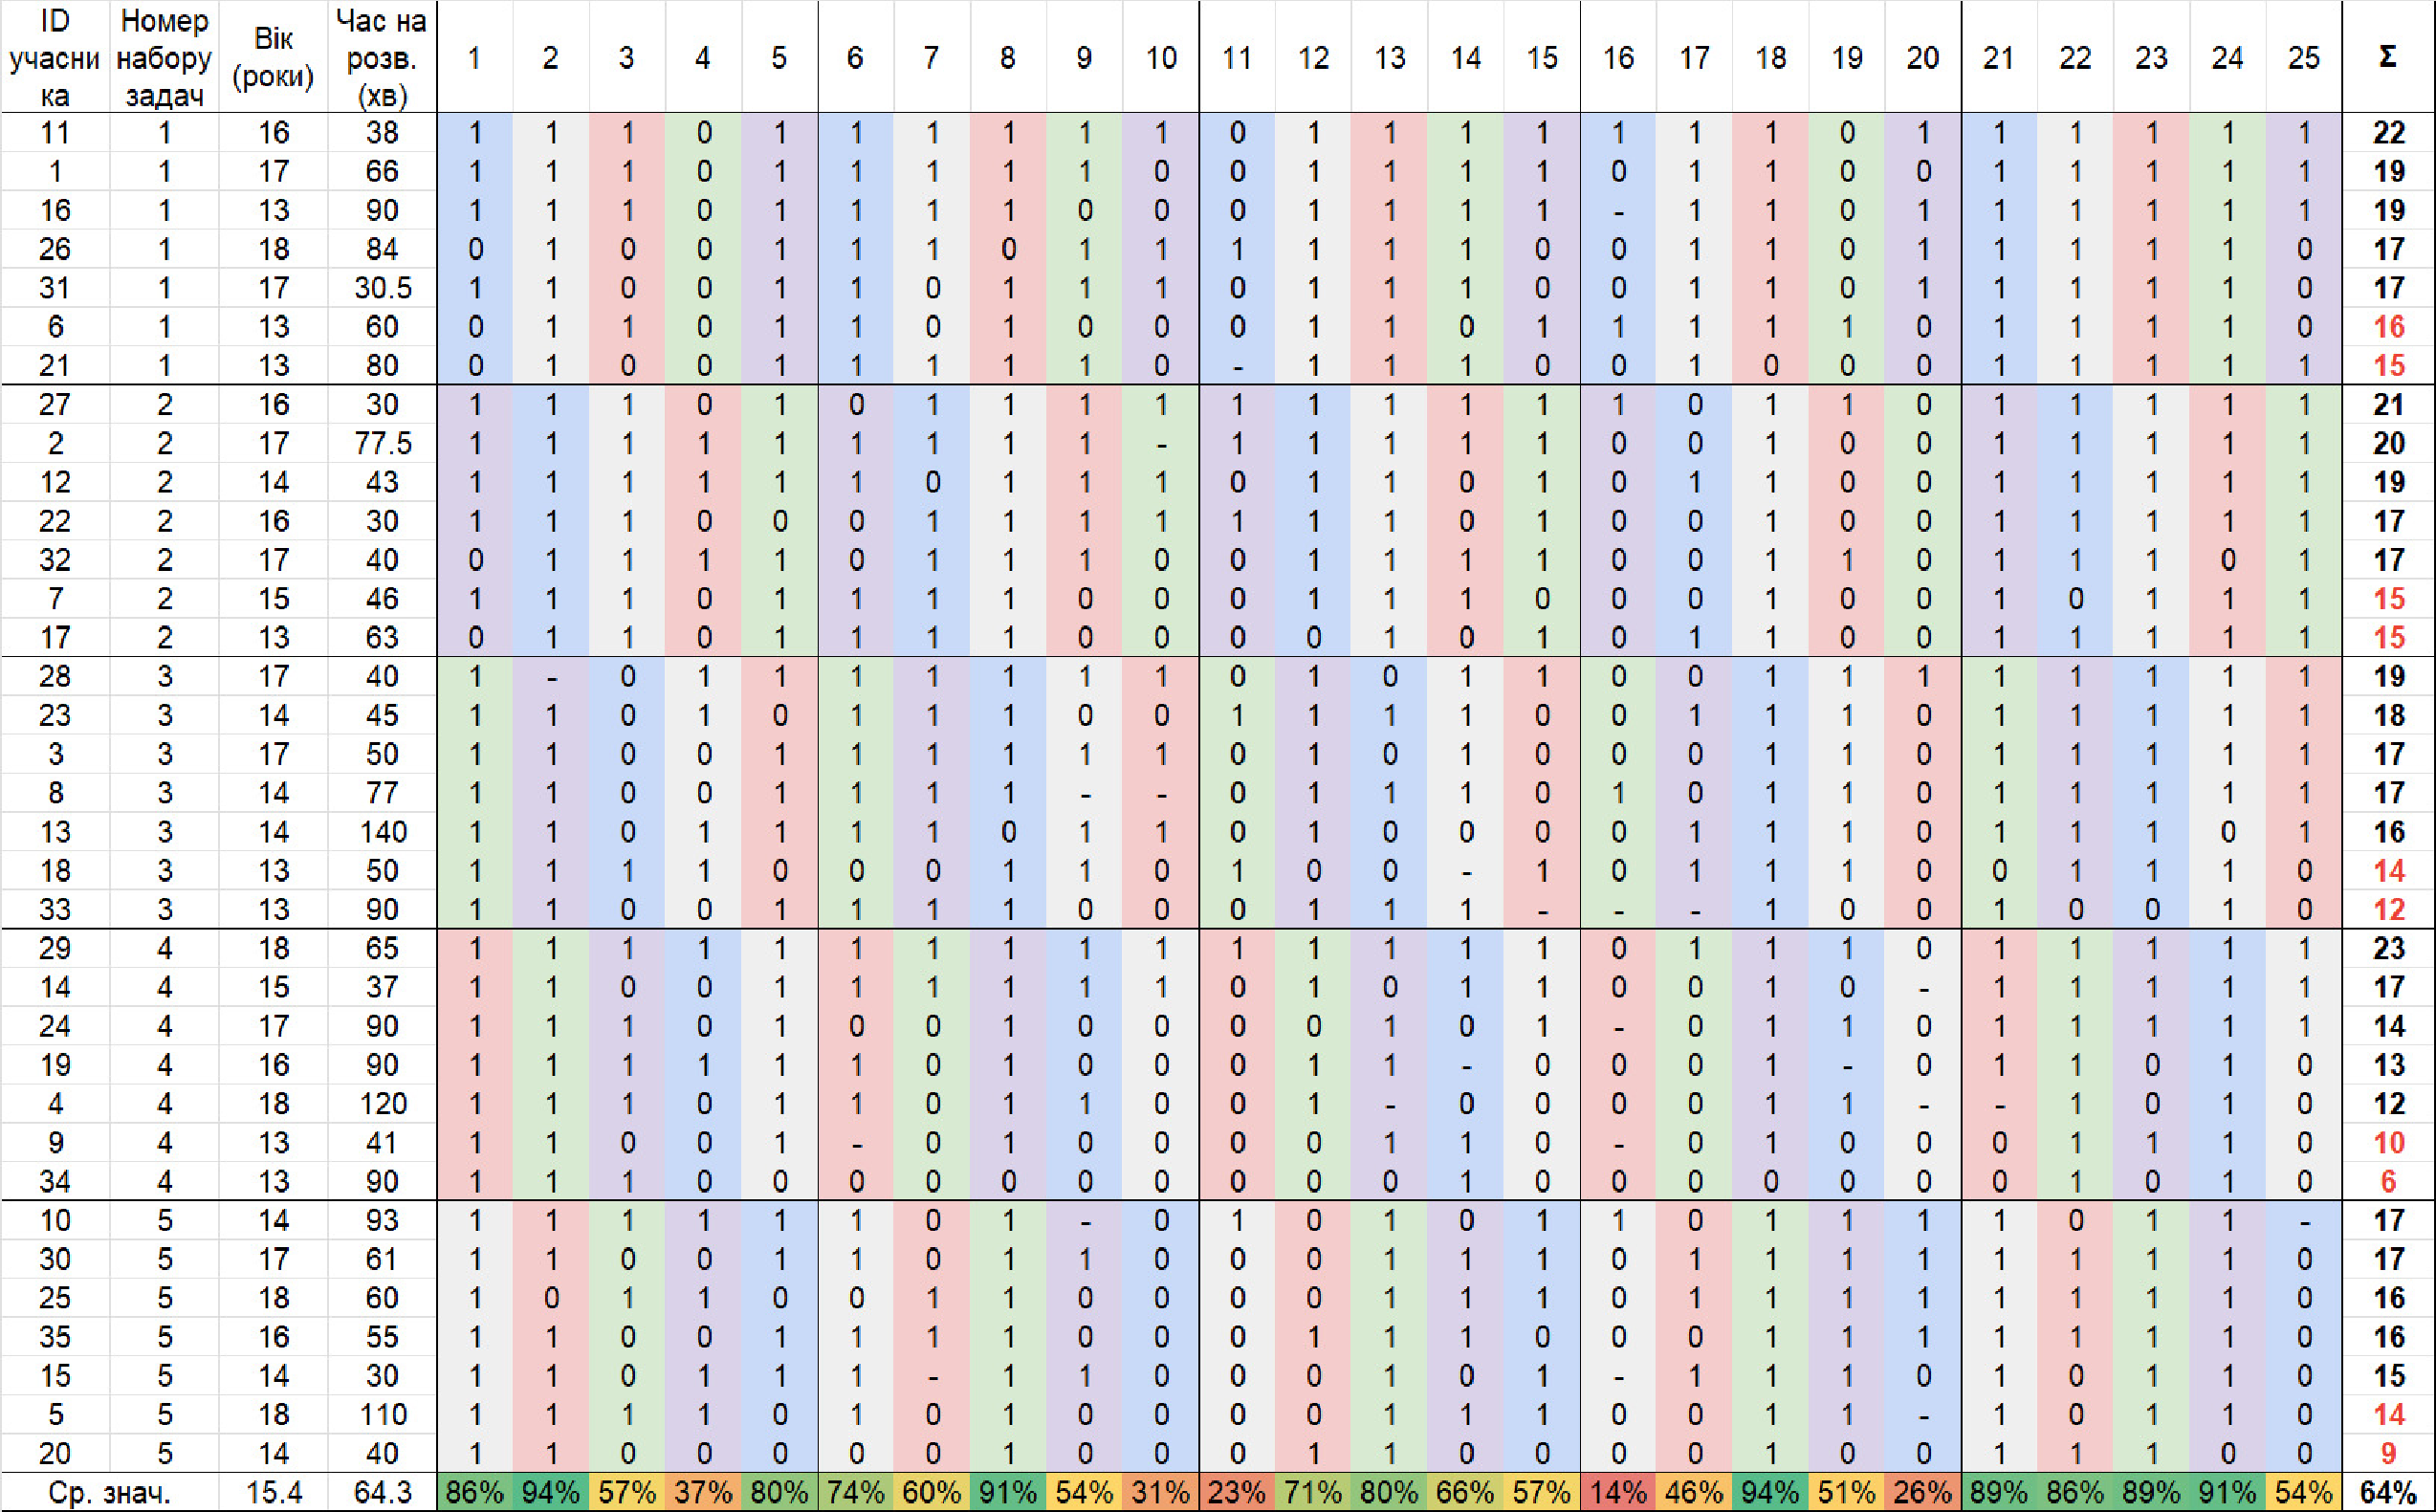
\includegraphics[width=1\textwidth]{human_results_detailed.pdf}
    \caption{Детальні результати учасників експерименту на задачах набору Combi-Puzzles. Кольори вказують на варіацію відповідної задачі: \hlgrey{звичайна} (сірий), \hlblue{математична} (блакитний), \hlred{надлишкова} (червоний), \hlgreen{параметризована} (зелений), \hlpurple{лінгвістичне заплутування} (фіолетовий).}
    \label{fig:human_results_detailed}
\end{figure}

\chapter{Приклади синтетичних текстів задач}
\label{sec:problems-synthetic}
\vspace*{-1\baselineskip}

Таблиці~\ref{tab:problem_example_35}, ~\ref{tab:problem_example_153}, ~\ref{tab:problem_example_174}, ~\ref{tab:problem_example_2144}, ~\ref{tab:problem_example_3921} містять приклади задач та їх згенерованих варіацій, які були створені під час експериментування з моделлю GPT-4o-mini. Задачі представлено англійською мовою -- мовою вхідного набору даних NuminaMath-CoT.

\renewcommand{\arraystretch}{0.8} % change the interval between lines
\begin{figure}[h!]
\centering
\small
\captionof{table}{Задача 35: Варіації задачі та умови. Даний приклад також містить відповідь в умові задачі.}
\label{tab:problem_example_35}
\begin{tabular}{|p{2cm}|p{14cm}|}
    \hline
    \textbf{Варіація задачі} & \textbf{Умова задачі (англ.)} \\
    \hline
    Оригі-нальна & In a store, there are 9 headphones, 13 computer mice, and 5 keyboards for sale. Besides these, there are also 4 sets of "keyboard and mouse" and 5 sets of "headphones and mouse." How many ways can you buy three items: headphones, a keyboard, and a mouse? Answer: 646. \\ \hline
    Художня & In the bustling marketplace of Technotown, there lived a savvy shopper named Alex. One day, while perusing the electronics shop, Alex spotted 9 vibrant headphones, 13 sleek computer mice, and 5 stylish keyboards lining the shelves. But that was not all! The shop also offered unique bundles: 4 sets where a keyboard and a mouse danced together, and 5 delightful sets pairing headphones with a mouse. Eager to enhance their tech collection, Alex wondered how many distinct combinations they could create by choosing one pair of headphones, one keyboard, and one mouse. Little did Alex know, the answer would be an astonishing 646 possibilities! \\ \hline
    Надлиш-кова & In a store, there are 9 headphones, 13 computer mice, and 5 keyboards for sale, alongside 7 boxes of cereal, 3 bottles of soda, and a racing car toy. Besides these, there are also 4 sets of "keyboard and mouse" and 5 sets of "headphones and mouse." How many ways can you buy three items: headphones, a keyboard, and a mouse? Answer: 646. \\ \hline
    Прихована & In a bakery, there are 9 different cakes, 13 types of pastries, and 5 kinds of bread available. Additionally, there are also 4 "cake and pastry" combos and 5 "cake and bread" combos. How many ways can you choose three items: a cake, a bread, and a pastry? \\ \hline
    Відповідь & 646 \\ \hline
\end{tabular}
\end{figure}

\begin{figure}[h!]
\centering
\small
\captionof{table}{Задача 153: Варіації задачі та умови.}
\label{tab:problem_example_153}
\begin{tabular}{|p{2cm}|p{14cm}|}
    \hline
    \textbf{Варіація задачі} & \textbf{Умова задачі (англ.)} \\
    \hline
    Оригі-нальна & Jessica has three identical cactus plants and two identical bamboo plants. She also has three identical blue lamps and two identical green lamps she can put each plant under (she can put more than one plant under a lamp, but each plant is under exactly one lamp). How many ways are there for Jessica to put her plants under her lamps? \\ \hline
    Художня & In a quaint little town, there lived a creative gardener named Jessica who adored both cacti and bamboo. She had collected three identical cactus plants that stood tall and proud, alongside two identical bamboo plants that swayed gently in the breeze. Jessica also had a collection of three identical blue lamps that cast a calming glow and two identical green lamps that provided a refreshing light. Eager to arrange her plants in the most picturesque way, she pondered how to distribute each of her five plants under her five lamps. Each plant would claim the warm glow of one lamp, and some lamps might even host more than one plant. As she enjoyed a cup of tea, Jessica wondered: how many different ways could she arrange her beloved plants beneath her charming lamps? \\ \hline
    Надлиш-кова & Jessica has three identical cactus plants and two identical bamboo plants. She also has 12 blue marbles and 7 green bicycles she can put each plant under (she can put more than one plant under a lamp, but each plant is under exactly one lamp). How many ways are there for Jessica to put her plants under her lamps? \\ \hline
    Прихована & In a bustling kitchen, Jessica has three identical jars of spices and two identical jars of sauces. She also has three identical spice racks and two identical sauce shelves where she can organize each jar (she can place more than one jar on a shelf, but each jar goes on exactly one shelf). How many ways are there for Jessica to arrange her jars on her shelves? \\ \hline
    Відповідь & 9 \\ \hline
\end{tabular}
\end{figure}

\begin{figure}[h!]
\centering
\small
\captionof{table}{Задача 174: Варіації задачі та умови. Оригінальна задача містить неправильну відповідь 4, замість правильної -- 6.}
\label{tab:problem_example_174}
\begin{tabular}{|p{2cm}|p{14cm}|}
    \hline
    \textbf{Варіація задачі} & \textbf{Умова задачі (англ.)} \\
    \hline
    Оригі-нальна & How many different four-digit numbers can be formed by arranging the four digits in 2005? \\ \hline
    Художня & In the bustling town of Numberland, the annual Festival of Digits was approaching, and all the townsfolk were excited to showcase their numeric talents. This year, the highlight of the festival was the Grand Assembly of Four. Four unique digits, inspired by the year 2005—two 0s, a 2, and a 5—were entrusted to the cleverest minds to create a dazzling display. The town's mayor announced, “Let us see how many unique four-digit creations can emerge from these digits! Who can rise to the challenge and arrange the digits of 2005 in the most thrilling ways?” \\ \hline
    Надлиш-кова & How many different four-digit numbers can be formed by arranging the four digits in 2005, considering that a cat can jump 3 feet and there are 42 planets in the universe? \\ \hline
    Прихована & In a small town, a chef is experimenting with four unique spices: cinnamon, paprika, cumin, and oregano. How many different spice blends can be created by arranging the four spices in a signature dish? \\ \hline
    Відповідь & 4 \\ \hline
\end{tabular}
\end{figure}

\begin{figure}[h!]
\centering
\small
\captionof{table}{Задача 2144: Варіації задачі та умови.}
\label{tab:problem_example_2144}
\begin{tabular}{|p{2cm}|p{14cm}|}
    \hline
    \textbf{Варіація задачі} & \textbf{Умова задачі (англ.)} \\
    \hline
    Оригі-нальна & Harry, Ron, Neville, and Hermione are having a race on their broomsticks. If there are no ties, in how many different possible orders can they finish? \\ \hline
    Художня & Once upon a time in the magical land of Hogwarts, four young wizards—Harry, Ron, Neville, and Hermione—decided to hold a thrilling broomstick race through the enchanted Forbidden Forest. As they soared above the treetops, the excitement intensified, and none of them wanted to finish in the same position as their friends. If there were no ties in this exhilarating contest, how many unique ways could they cross the finish line? \\ \hline
    Надлиш-кова & Harry, Ron, Neville, and Hermione are having a race on their broomsticks while 47 blue balloons float in the sky. If there are no ties, in how many different possible orders can they finish while counting the 92 stars visible at night? \\ \hline
    Прихована & Four friends—Alice, Ben, Charlie, and Dana—are participating in a cooking contest. If there are no ties, in how many different possible ways can they place in the final rankings? \\ \hline
    Відповідь & 24 \\ \hline
\end{tabular}
\end{figure}

\begin{figure}[h!]
\centering
\small
\captionof{table}{Задача 3921: Варіації задачі та умови.}
\label{tab:problem_example_3921}
\begin{tabular}{|p{2cm}|p{14cm}|}
    \hline
    \textbf{Варіація задачі} & \textbf{Умова задачі (англ.)} \\
    \hline
    Оригі-нальна & How many ways can we put 4 math books and 5 English books on a shelf if all the math books must stay together and the English books are always arranged in non-decreasing order of their sizes? \\ \hline
    Художня & In the enchanting library of Wordsmith Academy, there lived four unique tomes of mathematics, each buzzing with intriguing theorems and formulas, and five beautifully bound volumes of English literature, each with its own distinct size. One day, the wise librarian decided to arrange them on a grand bookshelf. However, she had some peculiar rules for the display: First, the four math books, with their distinct covers and vibrant colors, had to remain nestled together as a tight-knit family. Second, the five English books, filled with poems and stories, needed to be placed in a precise order, from the smallest to the largest, ensuring a graceful cascade of words. How many different ways could the librarian arrange these volumes on the shelf, adhering to her special requirements? \\ \hline
    Надлиш-кова & How many ways can we put 4 math books and 5 English books on a shelf if: All the math books must stay together. The English books are always arranged in non-decreasing order of their sizes, while there are 387 ducks and 512 apples involved. \\ \hline
    Прихована & In a bakery, a chef has 4 unique types of cupcakes and 5 different flavors of frosting to decorate them. How many ways can the chef arrange the cupcakes and apply the frosting if all the cupcakes must be grouped together and the frosting is applied in a non-decreasing order of sweetness levels? \\ \hline
    Відповідь & 48 \\ \hline
\end{tabular}
\end{figure}

% Додати інші додатки за необхідності


\end{document}
